\documentclass[11.5pt]{article}
\usepackage{charter}
\usepackage{fullpage}
\usepackage[colorlinks=false]{hyperref}
\usepackage{ifthen}
\usepackage{comment}
\usepackage[title,titletoc]{appendix}

\bibliographystyle{unsrt}
\usepackage{color}
\usepackage{titlesec}
\usepackage{tikz}
\usepackage{tikzscale}
\usepackage{pgfplots}
\usepackage{nomencl}
\usepackage{amsfonts, booktabs,siunitx}
\usepackage{threeparttable}
\makenomenclature

\usepgflibrary{arrows}
\usetikzlibrary{snakes}
\usetikzlibrary{shapes.geometric}
\usetikzlibrary{patterns}
\usetikzlibrary{shapes,arrows,chains}
\usepgfplotslibrary{patchplots,colormaps}
\usetikzlibrary{calc}
\usetikzlibrary{positioning, fit}
\usetikzlibrary{backgrounds}
\usetikzlibrary{intersections}
\usepackage[]{algorithm2e}

\usepackage{flafter}


\newcommand{\todo}[1]{{\color{blue}#1}}
\newcommand{\cmnt}[1]{{\color{red}#1}}

\newcommand{\sectionbreak}{\clearpage}

\usepackage{indentfirst}

% math and cite
\newtheorem{thm}{Theorem}
\newtheorem{defn}{Definition}
\newcommand{\refsec}[1]{\S\ref{#1}}
\usepackage{soul}
\usepackage{amsmath}
\usepackage{url}
\usepackage{amsfonts}
\usepackage{amssymb}
\usepackage{amsthm}
\usepackage{soul}
\usepackage{fullpage}
\usepackage[noend]{algorithmic}
\usepackage{subfigure}
\usepackage[american]{babel}
%\usepackage{csquotes}
\usepackage{biblatex}
\usepackage{listings}


\lstset{emph={long, contract, return, uint256, bool, function, if, true,
    else, using, returns, constant, string, public, namespace, struct, for,
    int,char, typedef, void, double, float, static_cast,
    new},emphstyle=\color{blue}\ttfamily, 					basicstyle=\ttfamily,
  moredelim=[is][\color{red}]{^}{^}}

%\lstset{language=C++,
                %basicstyle=\ttfamily\footnotesize,
                %keywordstyle=\color{blue}\ttfamily\footnotesize,
                %stringstyle=\color{red}\ttfamily\footnotesize,
                %commentstyle=\color{green}\ttfamily\footnotesize,
                %morecomment=[l][\color{magenta}]{\#}
%}
%\lstset{%
  %escapeinside={(*}{*)},%
%}


\renewbibmacro*{name:andothers}{% Based on name:andothers from biblatex.def
  \ifboolexpr{
    test {\ifnumequal{\value{listcount}}{\value{liststop}}}
    and
    test \ifmorenames
  }
    {\ifnumgreater{\value{liststop}}{1}
       {\finalandcomma}
       {}%
     \andothersdelim\bibstring[\emph]{andothers}}
    {}}

    \addbibresource{reference.bib}






%\addbibresource{reference.bib}

\begin{document}

% ---------------------------------
% Los siguientes comandos son un quickfix para la imposibilidad de compilar este documento usando Babel.
\renewcommand\contentsname{Tabla de contenidos}
\renewcommand\refname{Referencias}
\renewcommand\appendixname{Anexo}
\renewcommand\appendixpagename{Anexos}
\renewcommand{\abstractname}{Resumen}
\renewcommand{\nomname}{Glosario}
\renewcommand{\figurename}{Fig.}
\renewcommand{\tablename}{Tabla}
\renewcommand{\baselinestretch}{1.5}
\newcommand{\dapp}{DApp\xspace}
\newcommand{\pidc}{Protocolo de Incentivos para Desarrolladores\xspace}
% ---------------------------------

\title{
	Libro blanco de Nebulas \\
	\large El sistema operativo con motor de búsqueda en blockchain basado en \textit{rankings}\\
	\small Título original: Nebulas Technical Whitepaper: The value-based blockchain operating system and search engine\\
	\small Traducción: Abril de 2019\\v1.0.0}
\author{Equipo Nebulas}
\date{Abril de 2018\\v1.0.2}

\maketitle

\newpage
\abstract{
比特币和以太坊系统分别给区块链世界带来“去中心化现金”和“智能合约”技术。相对于3年前,区块链技术及产业已经取得了长足的发展和繁荣。但是我们发现,在和现有商业及用户需求逐步结合的同时,已有的技术并不完美,面对着越来越多的挑战。

本文介绍了星云链的技术架构设计,意图构建一个基于价值尺度,并带有价值激励机制,具备自进化能力的区块链系统,主要内容包括:

\begin{itemize}
	\item \textbf{定义价值尺度的Nebulas Rank}(\refsec{sec:rank}),通过综合考虑链中各个账户的流动性、传播性和互操作性,Nebulas Rank试图为每个账户建立一个可信、可计算和可复现的普适价值尺度刻画。利用NR,将会有更多的应用可以结合自身场景,来挖掘更大纵深的公链价值。
	\item \textbf{基于价值尺度的PoD贡献度证明共识算法}(\refsec{sec:pod}),为了公链生态健康自由发展出发,星云链提出了共识算法的三个重要指标,即快速、不可逆和公平性,PoD通过融合PoS和PoI的优势,结合NR,在优先保证快速和不可逆的前提下,率先加入了公平性的考量。
	\item \textbf{支持核心协议和智能合约链上升级的星云原力Nebulas Force}(\refsec{sec:nebulasforce}),帮助公链本身和链上应用实现自我进化,动态调优适应市场变化,将会有更快的发展速度和更大的生存潜力,有能力构建更宏伟的愿景。
	\item \textbf{DIP开发者激励协议}(\refsec{sec:dip}),为了更好地建立区块链应用生态环境,星云链将通过星云币的奖励来感谢为⽣态助⼒的优秀智能合约开发者,促进公链更加丰富多元的价值沉淀。
	\item \textbf{智能合约搜索引擎}(\refsec{sec:search})。
\end{itemize}
} %TRADUCIDO
\tableofcontents

\printnomenclature


\nomenclature{NR}{Nebulas Rank,星云指数排名}%
\nomenclature{NF}{Nebulas Force,星云原力}%
\nomenclature{SCDS}{Smart Contract Devotion Score,智能合约贡献度评分}%
\nomenclature{SCDR}{Smart Contract Devotion Rank,智能合约贡献度排名}%
\nomenclature{PoW}{Proof of Work,工作量证明}%
\nomenclature{PoS}{Proof of Stake,股权证明}%
\nomenclature{PoI}{Proof of Importance,重要度证明}%
\nomenclature{PoD}{Proof of Devotion,贡献度证明}%
\nomenclature{DIP}{Developer Incentive Protocol,开发者激励协议}%
\nomenclature{WAA}{Weekly Active Address,周活跃地址}%
\nomenclature{BFT}{Byzantine Fault Tolerant,拜占庭容错算法}%
\nomenclature{NNS}{Nebulas Name Service,星云链域名服务}%

\renewcommand{\nomname}{术语表}
 %TRADUCIDO
\newpage
\section{简介}

\subsection{区块链技术简介}
区块链技术来源于比特币\cite{Nakamoto2008},比特币的概念最初由中本聪在2008年提出,是一种去中心化的数字货币。比特币不依靠特定货币机构发行,根据特定算法,依靠大量计算产生。产生的过程实质上是用计算机解决一项复杂的数学问题,来保证比特币网络分布式记账系统的一致性。区块链是以比特币为代表的数字加密货币体系的核心支撑技术,能够通过运用数据加密、时间戳、分布式共识和经济激励等手段,在节点无需互相信任的分布式系统中实现去中心化信用的点对点交易、协调与协作,从而解决中心化机构普遍存在的高成本、低效率和数据存储不安全等问题。需要说明的是,区块链技术本身不是一个全新的技术创新,而是作为一系列技术的组合(包括点对点通讯,密码学,块链数据结构等)产生的模式创新。

\subsection{商业和技术挑战}
区块链技术为代表的去中心化,自主治理的系统,正在引起越来越多人的重视和研究。当前全球区块链项目已经超过2000个,全球加密数字资产总体价值达到900亿美元。区块链\&数字资产领域的用户人群也正在快速增加。从2013年初的全球200万用户,到2017年初的2000万用户。我们认为,在2020年左右,全球区块链/数字资产用户会达到或超过2亿。在2025年前后,全球用户有望达到10亿规模。在这种规模下,区块链技术面临诸多的挑战,比如区块链信息的交互、协议的升级,以及区块链应用和智能合约的有效及相关性判断问题。

\paragraph{区块链信息的交互}即互操作性不足的问题,行业内已经有很多共识,迄今为止还没有完善的解决方案。主要是关于链内及链外,同时也包括“跨链”的数据及资产交互问题,这极大程度的限制了区块链的发挥空间,形成所谓区块链内外的“信息孤岛”。我们也看到,越来越多的区块链项目尝试对此有所突破。同时,对于不同区块链上的信息\&资产当前缺少统一的协议和标准,导致各区块链系统内外部的互操作性严重不足。

\paragraph{区块链系统协议的升级}不同于普通软件的版本迭代,往往会引发区块链“硬分叉”或“软分叉”。以比特币为例,社区关于区块扩容至今仍然存在巨大的争议,导致比特币协议进化缓慢,区块容量严重不足,出现过近100万笔交易在交易池等待被写入区块。目前来看比特币转账时间存在很大不确定性,用户很多时候不得不额外支付高昂的“交易加速费”,严重损害体验。另外,从以太坊的“硬分叉”来看,虽然暂时解决了问题,但是产生了ETH和ETC“重资产”和社区分裂的“副作用”。

\paragraph{区块链应用及智能合约的高效检索}随着区块链上各种应用(DApp)的快速增长,逐渐成为一个巨大的挑战。举以太坊为例,基于以太坊的DApp总数已经数十万个,试想如果区块链世界DApp接近App Store里应用总量规模的话,如何发现并找到好用的DApp就是个很大问题。从这里来看,当前区块链世界缺乏更多维度的信息和价值评判尺度,用来帮助用户更好的探索区块链世界。

\subsection{星云链设计原则}
面对上述机遇和挑战,我们要设计一个基于价值激励的自进化区块链系统。具体来说,我们有以下设计原则:
\begin{itemize}
	\item 完全兼容以太坊

以太坊已经有巨大的生态,是一个非常成功的公有区块链平台。星云链希望尽可能的借鉴以太坊优秀的设计,从协议底层以及智能合约编程上完全兼容以太坊,使得基于以太坊开发的产品能够零成本的迁移到星云链上。

	\item 公正的排序算法,定义价值尺度

我们认为,区块链世界需要一个普适的价值尺度,用于衡量区块链底层简单数据的价值,发现信息的更高维度,从而探索并挖掘区块链世界的更大价值。类似Google的PageRank\cite{Brin2010}\cite{page1999pagerank},我们也提出区块链世界的NR(Nebulas Rank)算法,综合考虑了区块链上的资金流动性,以及资金传播的速度、广度和深度,给区块链用户做公正的排序。NR是星云链赋予区块链世界的价值尺度,用来衡量区块链中各个用户、智能合约、DApp的重要性。NR有巨大的商业潜力,可以用在搜索、推荐、广告等领域当中。

	\item 更快更合理的共识算法

区块链的分布式交易总账需要在尽可能短的时间内做到安全、明确及不可逆,需要一个坚实的共识算法。目前主流的共识算法都各自存在一些缺陷,如PoW (Proof of Work)工作量共识,需要消耗大量的计算资源,影响共识速度;PoS (Proof of Stake)股权证明共识,容易形成大资本垄断,破坏生态平衡;PoI (Proof of Importance)重要性证明共识,存在nothing-at-stake~\cite{nothingatstake}的问题。 

在星云链中,我们提出了基于账户声望的PoD(见\refsec{sec:pod})算法,利用NR的价值尺度评估找出拥有影响力高声望的账户,平等地赋予记账资格,遏制记账权被垄断,然后融合PoS中的经济惩罚,防止公链被恶意破坏,为生态自由发展助力。

	\item 核心协议的可升级,实现自我进化

我们认为,一个良态的区块链系统应该能够实现自我进化。在较少外部干涉的情况下,实现更快的计算、更强的系统、及更好的体验。星云链在区块结构上进行更好的设计,使得核心协议的升级能够通过区块数据的更新实现,不需要代价高昂的软、硬分叉。星云链具备自我升级进化的设计,未来比其它的公有链具有更快的发展速度,更大的生存潜力。

	\item 对区块链生态的有效激励

在星云链中,我们提出面向智能合约和DApp开发者的DIP(Developer Incentive Protocol, 开发者激励协议)(见\refsec{sec:dip})。DIP的核心思想是对社区贡献度高的智能合约或DApp的开发者,给予他们相应的开发者激励。激励由记账人负责写入区块。

普通公有链系统仅仅对记账人(矿工)奖励,星云链不仅奖励矿工,还奖励优秀的智能合约开发者。借助于DIP的正向反馈机制,更多的开发者将被持续激励创造更高价值的智能合约和DApp,从而构建面向开发者社区的正向反馈生态。

	\item 图灵完备、可升级的智能合约

目前公有链的智能合约不具有升级的能力,如果开发过程中没有认真审核的话,很难避免人工失误,一旦被黑客找到漏洞,损失往往是巨大的。2016年6月,The DAO攻击事件,由于一个代码缺陷,导致以太坊用户损失了共计6000万美元的损失;最近Parity钱包的漏洞,导致15万个以太币的流失,价值3000万美元。以太坊由于The DAO的攻击,不得不进行硬分叉,造成很多诟病:一个设计不好的智能合约,绑架了整个区块链生态。星云链希望从底层提供智能合约升级的能力,面对漏洞,能够更快的响应和升级,不再需要区块链强行分叉来应对黑客事件。

\end{itemize}

 %TRADUCIDO
\newpage
\section{Nebulas Rank}
\label{sec:rank}

\subsection{Introducción a Nebulas Rank} \label{subsec:value}
Actualmente la tecnología blockchain y su comunidad han crecido hasta llegar a ser un ecosistema a gran escala. Sin embargo, la percepción popular de blockchain en el mundo es todavía algo superficial; no existe aún una forma razonable de evaluar el valor de una entidad (tal como la dirección de un usuario) en el blockchain. Por ende, trabajamos para elaborar una medida universal de valor. Mediante la exploración y el uso de actividades en el blockchain, hemos creado \textbf{Nebulas Rank} un algoritmo a través del cual se puede cuantificar el valor de cada entidad (como la dirección de un usuario). \textbf{Nebulas Rank} está diseñado para:\begin{itemize}
	\item servir como una medida nativa de valor y como un algoritmo central para distintos escenarios fundamentales, como el algoritmo de consenso (véase \refsec{sec:pod}), el Protocolo de Incentivos a Desarrolladores (véase \refsec{sec:dip}) y el motor de búsquedas de blockchain (véase \refsec{sec:search}), entre otros;
	\item inspirar valuaciones diversas y percepciones más profundas en el ecosistema blockchain, de modo de guiar con más precisión las decisionesde negocios y las actividades de investigación.
\end{itemize}
Basándonos en las metas arriba mencionadas, podemos definir la medición de valor de \textbf{Nebulas Rank} desde tres \textit{dimensiones}:
\begin{itemize}

	\item \textbf{Liquidez}, la frecuencia y escala de las transacciones es la primera dimensión que mide \textbf{Nebulas Rank}. Las finanzas son esencialmente actividades que optimizan los recursos sociales a través de la liquidez del capital y que promueven el desarrollo económico. Blockchain establece una red de valor, en el sentido de que a mayor cantidad y escala de transacciones se logra una mayor liquidez, lo que aumenta aún más las transacciones y su escala, formando así un círculo virtuoso.

	\item \textbf{Propagación}, el alcance y la profundidad de la liquidez de los activos es la segunda dimensión que mide \textbf{Nebulas Rank}. En las redes sociales la propiedad de propagación —es decir: la velocidad, el alcance y la profundidad de la transmisión de la información— es un índice clave que muestra la calidad de la red y el crecimiento de los usuarios. El mismo patrón se puede observar en el mundo blockchain: una propagación de gran alcance implica una liquidez de activos más amplia y profunda, lo que mejora la calidad y la escala de los activos.

	\item \textbf{Interoperabilidad} es la tercera dimensión que mide textbf{Nebulas Rank}. Durante la primera etapa de Internet, sólo existían sitios web sencillos y la información estaba aislada. En la actualidad la información se puede enviar desde distintas plataformas y es cada vez más raro encontrar información aislada. Esta tendencia podría entenderse como un proceso de reconocimiento de la información desde una perspectiva dimensional superior. Creemos que el mundo blockchain también sigue un patrón similar, aunque su desarrollo es más rápido. Habrá más información disponible sobre los activos de los usuarios, sobre contratos inteligentes y sobre {\dapp}s. Y, además, todas esas entidades interactuarán con más frecuencia. Por lo tanto, es cada vez más importante que exista una mejor interoperabilidad en el blockchain.

\end{itemize}

Elegimos los registros de transacciones en blockchain como el origen de datos para \textbf{Nebulas Rank} debido a que la \textit{trayectoria} en el mundo de blockchain es más clara y confiable que la del mundo real. Los datos de las transacciones —como las transferencias y las llamadas a contratos inteligentes— quedan registradas en el blockchain. Aun así, no es trivial diseñar algoritmos de valuación para los datos de transacciones en el blockchain, ya que éstas son naturalmente anónimas y poseen una mayor escala de datos que en el mundo real.

A continuación se describen tres propiedades principales para \textbf{Nebulas Rank}:

\begin{itemize}

	\item Veracidad. Una entidad debe pagar un costo razonable para mejorar su valuación, lo que asegura que el algoritmo pueda identificar a los usuarios legítimos y valiosos. Por un lado, en escenarios como el algoritmo de consenso y el DIP, una valuación veraz anima a los usuarios a contribuir de manera honesta con el fin de obtener un \textit{feedback} positivo. Por otro lado, un resultado veraz proporciona una representación jerárquica significativa de todos los usuarios, lo que será útil para los responsables de tomar decisiones;

	\item Computabilidad. Al ser un indicador fundamental, es vital que el resultado de \textbf{Nebulas Rank} sea accesible instantáneamente, lo que requiere una baja complejidad computacional;

	\item Determinismo. Tal como es requerido en escenarios como el algoritmo de consenso y el DIP, el resultado del cálculo de \textbf{Nebulas Rank} debe ser idéntico y replicable en cualquier cliente.

\end{itemize}

Next, we design the basic framework of \textbf{Nebulas Rank}. First, transaction records are represented in the form of graph. In the transaction graph (entity graph), every node is mapped to one entity, and each edge represents the transfer between two entities\cite{Tschorsch2015}. Transaction graph embodies the fact that money transfer among users leads to assets flowing, which helps to represent the concepts of liquidity and propagation defined before. Meanwhile, the form of graph can clearly display the interoperability among contracts. With the derived transaction graph, we rank nodes by their network centrality. In the scenario of \textbf{Nebulas Rank}, LeaderRank\cite{Chen2013}\cite{Li2014} is a more reasonable measurement and outperforms PageRank of Google and NCDAwareRank of NEM\cite{nem}.

\subsection{Transaction Graph} \label{subsec:txg}
This subsection introduces how to derive transaction graph from transaction history.

First, for any time $t_0$, we take all \textbf{effective} transactions among individual addresses during $[t_0- T, t_0]$ ($T$ is a constant, generally set to one month), where every transaction can be represented as a 4-tuple $(s,r,a,t)$, with $s$ as the source address, $r$ as the target address, $a$ as the transfer amount and $t$ as the block time. We define a transaction to be \textbf{effective} iff $a>0$ and $s \neq r	$. Thus all \textbf{effective} transactions during $[t_0- T, t_0]$ can be represented by a set of 4-tuples:

\begin{align}
\Theta(t_0) = \{(s, r, a, t)\ |\ t_0 - T \le t \le t_0\ \land \ a > 0 \land s \neq t \}
\end{align}

Then based on $\Theta(t_0)$, construct a directed weighted simple graph $G=(V,E, W)$, where node set, edge set and edge weights are denoted by $V$, $E$ and $W$ respectively. Every node in $V$ represents an individual account's address, and each edge in $E$ represents the transfer intensity between two addresses. Edges are directed and are assigned with weight $w_e$ aggregating top $K$ amounts of all related transactions:
\begin{align}\label{formula:edgeweight}
w_e = \sum_{i=1}^K a_i,\ s.t.\ a_i \in A_e
\end{align}
$A_e$ is an ordered set consisting of amounts of all transactions from $s$ to $r$ in $\Theta(t_0)$:
\begin{align}
A_e = \{a_i\ |\ e = (s,r) \land (s, r, a_i, t) \in \Theta(t_0) \land (a_i \ge a_j, \forall i \le j) \}
\end{align}

Additionally, let $N = |V|$,$M = |E|$, where $|.|$ is the cardinal number of a set. For simplicity, every node is represented by an integer between $1$ and $N$.

\begin{figure}[h]
\centering
	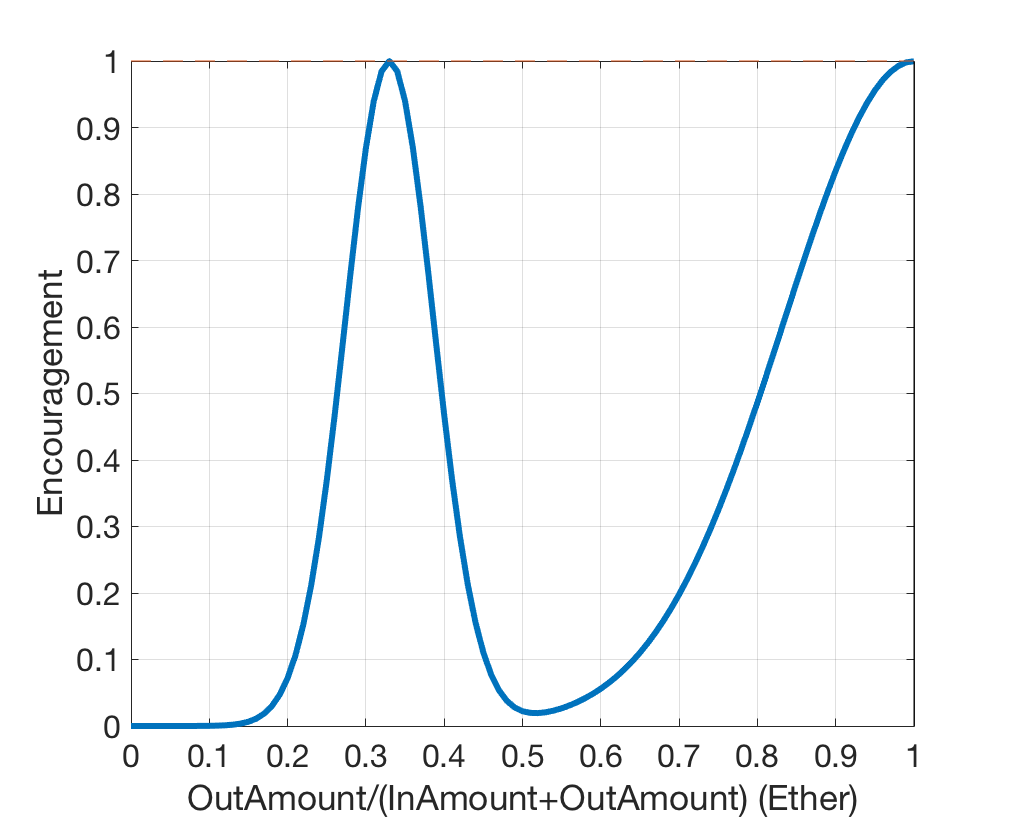
\includegraphics[width=0.55\textwidth]{figs/encouragement_en.png}
	\caption{Encouragement Function}\label{fig:encouragement}
\end{figure}

Then, for each node, according to its in-transfers and out-transfers during $[t_0\ —\ T,\ t_0]$, compute the ``coinage" and denote it by $C_v$; based on the total transfer amount and using the ``encouragement function" shown in \reffig{fig:encouragement}, compute the encouragement value and denote it by $E_v$\footnote{Encouragement function can be represented as a linear combination of two normal distributions, which outputs peak value when the money transferred out is zero or of some ratio of the amount transferred in.}; use $C_v$ and $E_v$ of the target nodes to reduce the edges' weight.

Finally, take the largest weakly connected component of the whole graph, only keep nodes belong to this component. The deleted nodes are assigned with lowest importance score by default.

The graph derivation described above contributes to the ``truthful" property defined at \refsec{subsec:value}, the evidence of which is shown in \refsec{subsec:robust}.

Using the method described herein, the transaction graph, wherein $T$ is 30 days and $K=2$, is created on the basis of transaction data in the main chain of Ethereum, from block \#3629091(roughly on May 1st, 2017) to block \#3800775(roughly on May 31st, 2017). Its visualization is shown as \reffig{fig:wgc}. , and all nodes are resized by their degree. It could be observed that some famous exchanges usually interacts with more accounts than others. Besides, the identities of some addresses who contribute a lot transactions still remains unknown.

\begin{figure}[htbp]
	\centering
	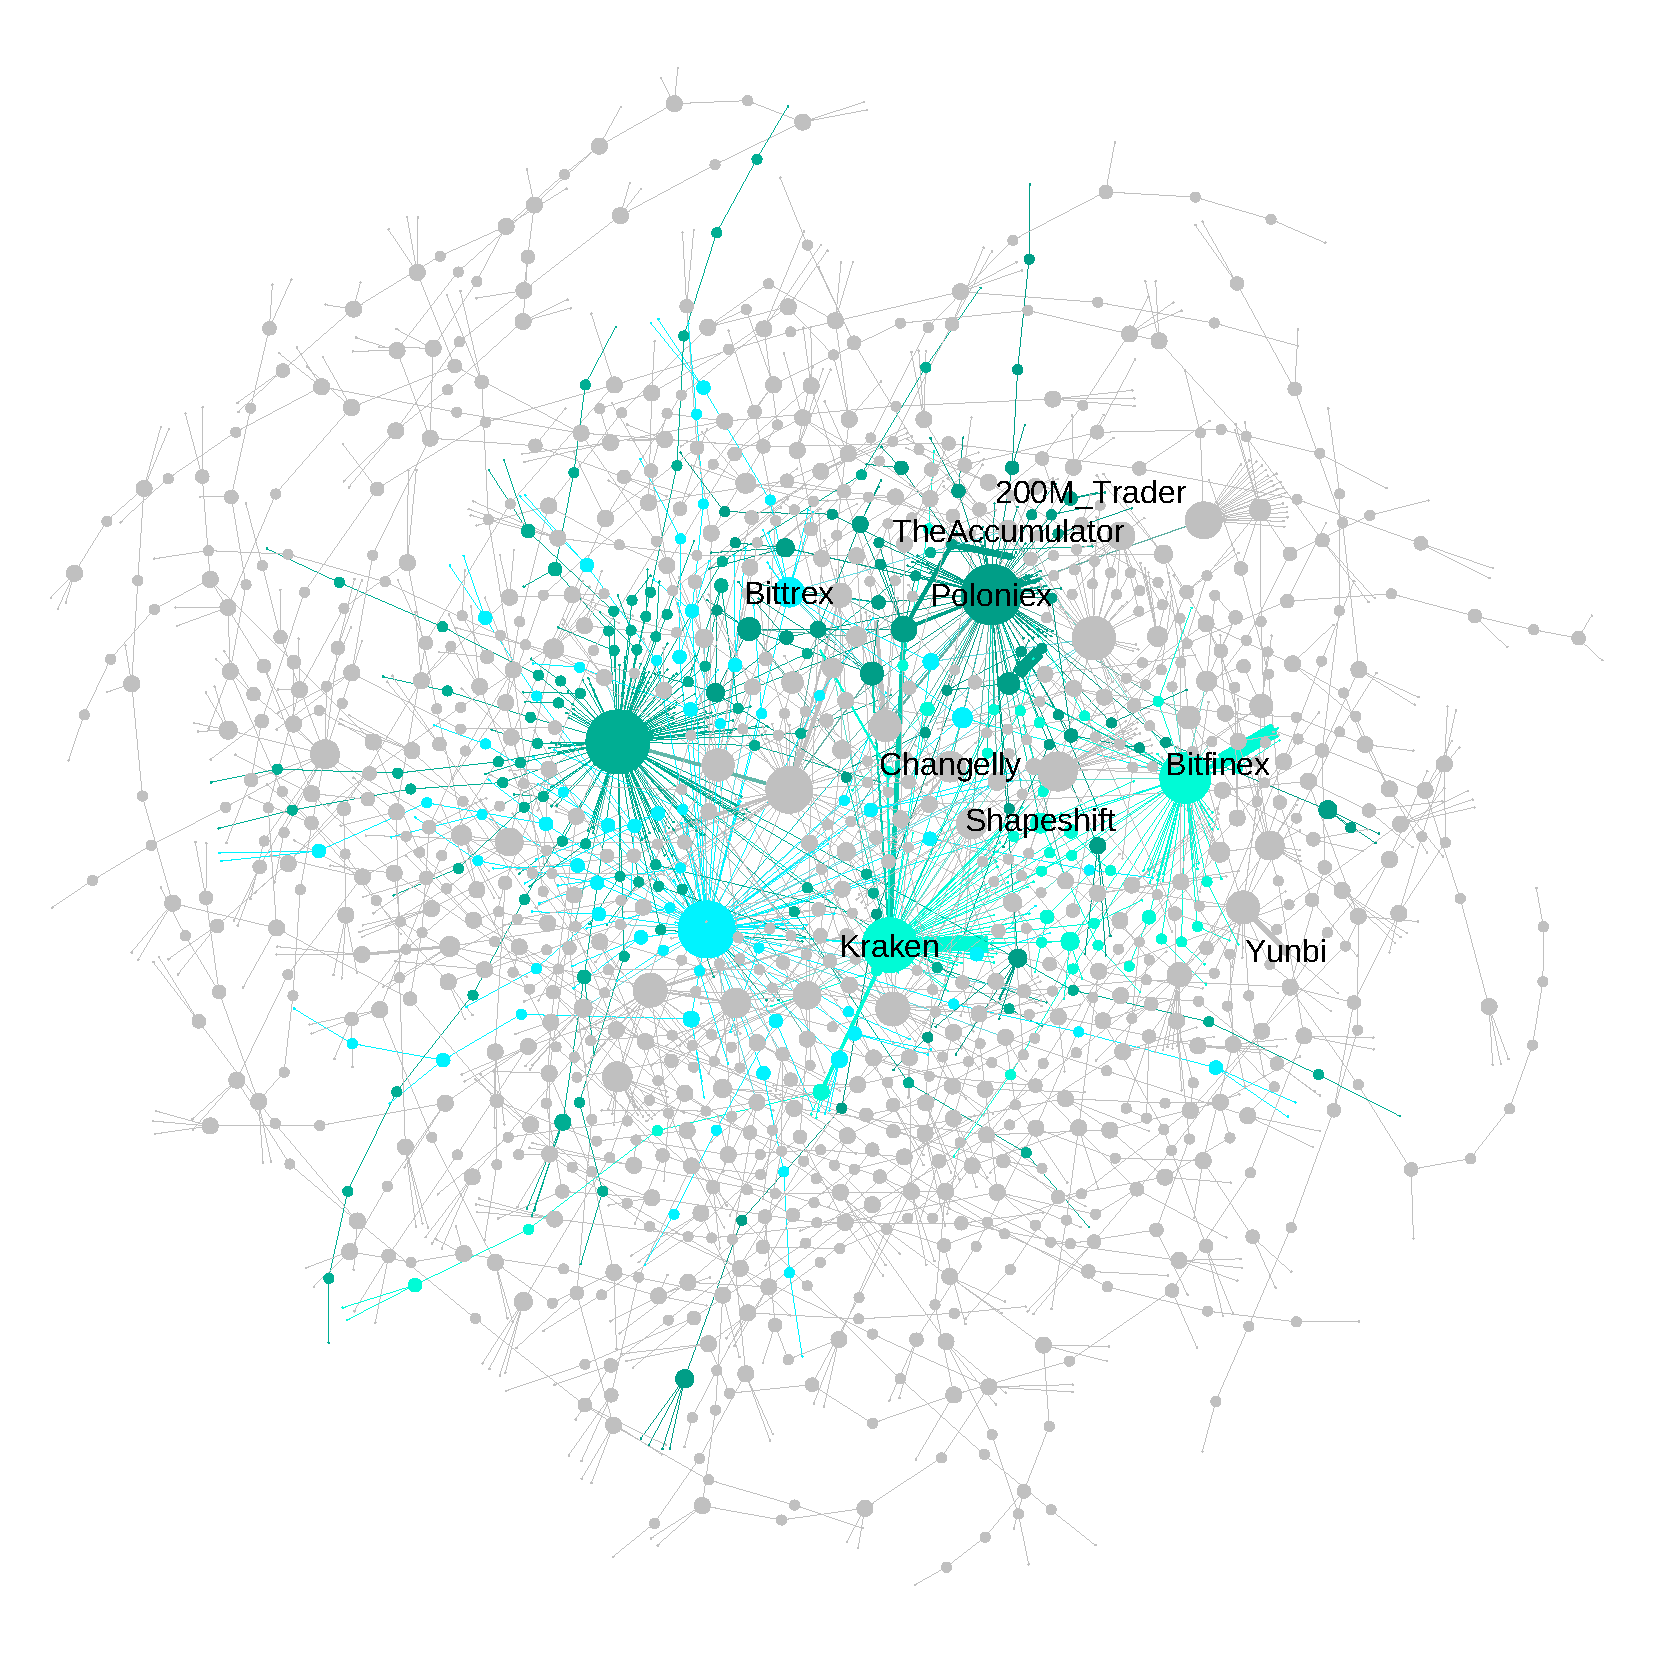
\includegraphics[width=0.85\textwidth]{figs/wgc1.png}
	\caption{Transaction Graph (Partial) Visualization. \small{Large transaction scale (capital transfer) in the address means high in-and-out degree in the node, represented by large diameter in the figure. Some nodes are labeled by tags according to Etherscan\cite{etherscan}}  }\label{fig:wgc}
\end{figure}

\subsection{Ranking Algorithm} \label{subsec:leaderrank}
This subsection introduces how to rank nodes by their importance in the derived transaction graph.

We adopt LeaderRank\cite{Chen2013}\cite{Li2014} as the main algorithm. First, add a ground node with index $0$ into the transaction graph. Then establish bi-directional link between the ground node $0$ and every other node $i$ ($1 \leq i \leq N$), weighting by the following formula:
\begin{align}\label{formula:weight1}
w_{i,0} = \alpha( max\{ \sum_{w_{j,i} \neq 0} w_{j,i} - \sum_{w_{i,j} \neq 0} w_{i,j} , 0\} + \lambda C ), \forall i \in [1,N]
\end{align}
\begin{align}\label{formula:weight2}
w_{0,i}	= \beta ( \sum_{w_{i,m} \neq 0} w_{i,m} + \mu C), \forall i \in [1,N]
\end{align}
$C$ is the median of set $\{w_{i,j} | w_{i,j} \neq 0, 0\leq i,j \leq N\}$, and $\alpha, \beta, \mu, \lambda$ are parameters.

The weighting scheme can be explained that, nodes with more in-degree receive more in-link from the ground node; nodes with more absolute income, i.e. in-degree minus out-degree, outputs stronger link into the ground node.

The computing process of LeaderRank is similar to PageRank, which could be understood as computing the convergence state of a Markov process. The only difference is that, after adding the ground node, it does not need to consider the damping factor of PageRank\cite{Brin2010}\cite{page1999pagerank} anymore. That is, after constructing matrix $H$ according to formula (\ref{formula:matrix}), the computing process is iterated until convergence, as formula (\ref{formula:iteration}) shows, with initial settings defined by formula (\ref{formula:init}). Finally the rank score of ground node is distributed evenly to every other node, which yields the final score for every node.
\begin{align} \label{formula:iteration}
	P^{t+1} = H \times P^{t}; P^1=[0, \frac{1}{N}, \frac{1}{N}, \dots, \frac{1}{N}]^T
\end{align}
\begin{align} \label{formula:matrix}
	h_{ij} = \frac{w_{(j,i)}}{\sum_k w_{(j,k)}}
\end{align}
\begin{align} \label{formula:init}
\forall v \in V, P^*_v \leftarrow P^*_v + \frac{P^*_{\mathcal{G}}}{N}
\end{align}

We suppose that LeaderRank can satisfy the measure of value and algorithm property defined in \refsec{subsec:value}.
\begin{itemize}
	\item The result of LeaderRank can be understood as the flux on each node in the dynamic equilibrium of money exchange network, which matches \textbf{Nebulas Rank}'s measure of value: ``liquidity", ``propagation" and ``interoperability";
	\item The weighing scheme defined by formula (\ref{formula:weight2}) and (\ref{formula:weight1}) makes it more difficult to attack (see discussion in \refsec{subsec:robust}), which satisfies ``truthful" property;
	\item LeaderRank can be computed by power iteration. Since the network is very sparse, the complexity of matrix computation should not be high, which satisfies the properties of ``computable" and ``deterministic".
\end{itemize}


\subsection{Manipulation Resistance}\label{subsec:robust}
Truthfulness, i.e. the ability of resisting manipulation, is the most significant and challenging goal of \textbf{Nebulas Rank}. Some manipulation methods are as follows:
\begin{enumerate}
	\item Loop transfer. The attacker transfers along a loop topology, which allows the same money flow over same edges repeatedly. By this means, the attacker hopes to raise the weight of related edges;
	\item Transfer to random addresses, so that the out-degree of sybil node is increased, and the propagation of fund is increased as well;
	\item Form an independent network component with addresses controlled by the attacker. So the attacker can pretend to be a central node;
	\item Interact with authoritative Exchange service addresses frequently, i.e. transfer the same money in and out an authoritative Exchange service address repeatedly, so that the attacker can acquire better structural position in the network.
\end{enumerate}

\textbf{Nebulas Rank} mitigates manipulation through the following mechanism:
\begin{itemize}
	\item Owing to sliding windows of $T$ blocks, the attacker cannot increase its rank in short term;
	\item Since the edge weight is decided by the related transactions with highest amount , transferring along a loop topology cannot increase edges' weight unlimitedly. Meanwhile, according to the sampled data in \refsec{subsec:txg}, $91\%$ of edges correspond to less than 2 transactions respectively. Thus $K=2$ is a reasonable choice to remain the intensity information on edges while being resistance to loop transfer;
	\item In order to have higher ``coinage", the user needs to let money stay in their address for a while, which slows down the attacking speed;
	\item In order to get the maximum ``encouragement value", as is shown in \reffig{fig:encouragement}, the account needs to spend more than income or transfer out only a small ratio of income. So when forging money flow, the attacker will get a rapid decrease in its deposit;
	\item Because only the giant component is selected, other independent components including the forged one will be filtered out as noise. According to the sampled data in \refsec{subsec:txg}, there are $453,285$ nodes and $970,577$ edges, with $1,169$ components. In the biggest component, there are $449,746$ nodes, accounting for $99.2\%$ of the total number. In the second biggest component, there are just $133$ nodes, only accounting for $0.03\%$. Thus taking the giant component can remain normal part of network as much as possible while filtering noise part out;
	\item Compared with webpage ranking algorithms such as PageRank and NCDawareRank\cite{Nikolakopoulos2013}, the mechanism defined by formula (\ref{formula:weight2}) and (\ref{formula:weight1}) is more ``conservative" on the nodes with low income, i.e. nodes with low in-degree get weaker links from the Ground node. In the blockchain transaction graph, nodes with low income are more likely to be generated, and transferring to other random nodes cannot raise in-degree. So \textbf{Nebulas Rank} can increase the difficulty of manipulation.
\end{itemize}

Next, the following conclusions are made based on the transaction graph of Ethereum in May, 2017.

First, some addresses by \textbf{Nebulas Rank} are listed in table \ref{table:nr}\footnote{Source of domain: Etherscan\cite{etherscan}}. It can be observed that the Exchange addresses and some accounts with high transaction throughput are ranked as top nodes.

%\newpage
\begin{table}[!htbp]
\centering
\caption{\textbf{Top 10} addresses of \textbf{Nebulas Rank} and some other addresses}
\label{table:nr}
\begin{tabular}{llllll}\toprule
\begin{tabular}[c]{@{}l@{}}Rank\\ (Order)\end{tabular} & Address                                                                                    & Nebulas Rank & Domain          & Out Amount(Ether) & In Amount(Ether) \\
1  & \begin{tabular}[c]{@{}l@{}}0x267be1c1d684f78cb4f\\ 6a176c4911b741e4ffdc0\end{tabular} & 0.449275     & Kraken\_4   & 3214232.06  & 350008.00   \\
2  & \begin{tabular}[c]{@{}l@{}}0xd4c5867cec094721aab\\ c3c4d0fd2f2ac7878c79a\end{tabular} & 0.093798     &             & 58000.00    & 100947.00   \\
3  & \begin{tabular}[c]{@{}l@{}}0x027beefcbad782faf69f\\ ad12dee97ed894c68549\end{tabular} & 0.049277     & QuadrigaCX  & 207440.11   & 65606.40    \\
4  & \begin{tabular}[c]{@{}l@{}}0x0ee4e2d09aec35bdf08\\ 083b649033ac0a41aa75e\end{tabular} & 0.046831     &             & 56465.00    & 60087.96    \\
5  & \begin{tabular}[c]{@{}l@{}}0xc257274276a4e539741\\ ca11b590b9447b26a8051\end{tabular} & 0.037628     &             & 1071105.93  & 1434106.72  \\
6  & \begin{tabular}[c]{@{}l@{}}0xa53e0ca7d246a764993\\ f010d1fde4ad01189f4e6\end{tabular} & 0.033488     &             & 7764.68     & 3201.00     \\
7  & \begin{tabular}[c]{@{}l@{}}0xf259e51f791e9ed26e8\\ 9b6cae4a7c6296bfbd0b8\end{tabular} & 0.033481     &             & 3307.00     & 7731.30     \\
8  & \begin{tabular}[c]{@{}l@{}}0xf195cac8452bcbc836a\\ 4d32cfb22235af4ac1e9c\end{tabular} & 0.026343     &             & 10863.87    & 2315.69     \\
9  & \begin{tabular}[c]{@{}l@{}}0x94435d12c51e19d5b5c\\ 8656763f9069d37791a1a\end{tabular} & 0.024970     &             & 12938.58    & 15858.90    \\
10 & \begin{tabular}[c]{@{}l@{}}0x7580ba923c01783115d\\ 79975d6a41b3d38eff8d5\end{tabular} & 0.021670     &             & 263000.00   & 364793.49   \\
16 & \begin{tabular}[c]{@{}l@{}}0xcafb10ee663f465f9d10\\ 588ac44ed20ed608c11e\end{tabular} & 0.004995     & Bitfinex\_1 & 360000.00   & 1435858.40  \\
51 & \begin{tabular}[c]{@{}l@{}}0xd94c9ff168dc6aebf9b\\ 6cc86deff54f3fb0afc33\end{tabular} & 0.000868     & yunbi\_1    & 1179224.74  & 1202539.53  \\
64 & \begin{tabular}[c]{@{}l@{}}0x70faa28a6b8d6829a4b\\ 1e649d26ec9a2a39ba413\end{tabular} & 0.000590     & Shapeshift  & 52501.81    & 651933.49   \\
\bottomrule
\end{tabular}
\end{table}
\newpage

Then, we observe the relationship between transaction amount and \textbf{Nebulas Rank}. Since blockchain transferring can be understood as network flow of ``money exchange", according to \cite{Borgatti2005}'s work, the degree of nodes, i.e. sum of adjacent edges' weights, is a proper centrality metric for such network flow. From the perspective of each node, the degree, i.e. transaction throughput amount (amount transferred in plus amount transferred out), represents local information within one hop and reflects the historical money flow over corresponding addresses. So it could be a baseline for ranking algorithms. The relationship between transaction amount and \textbf{Nebulas Rank} is shown in \reffig{fig:nrio}: no node can acquire high rank with low transaction amount; nodes with high transaction amount still need to meet some conditions to get high rank, which roughly confirms the truthfulness of \textbf{Nebulas Rank}.
\begin{figure}[!htbp]
	\centering
	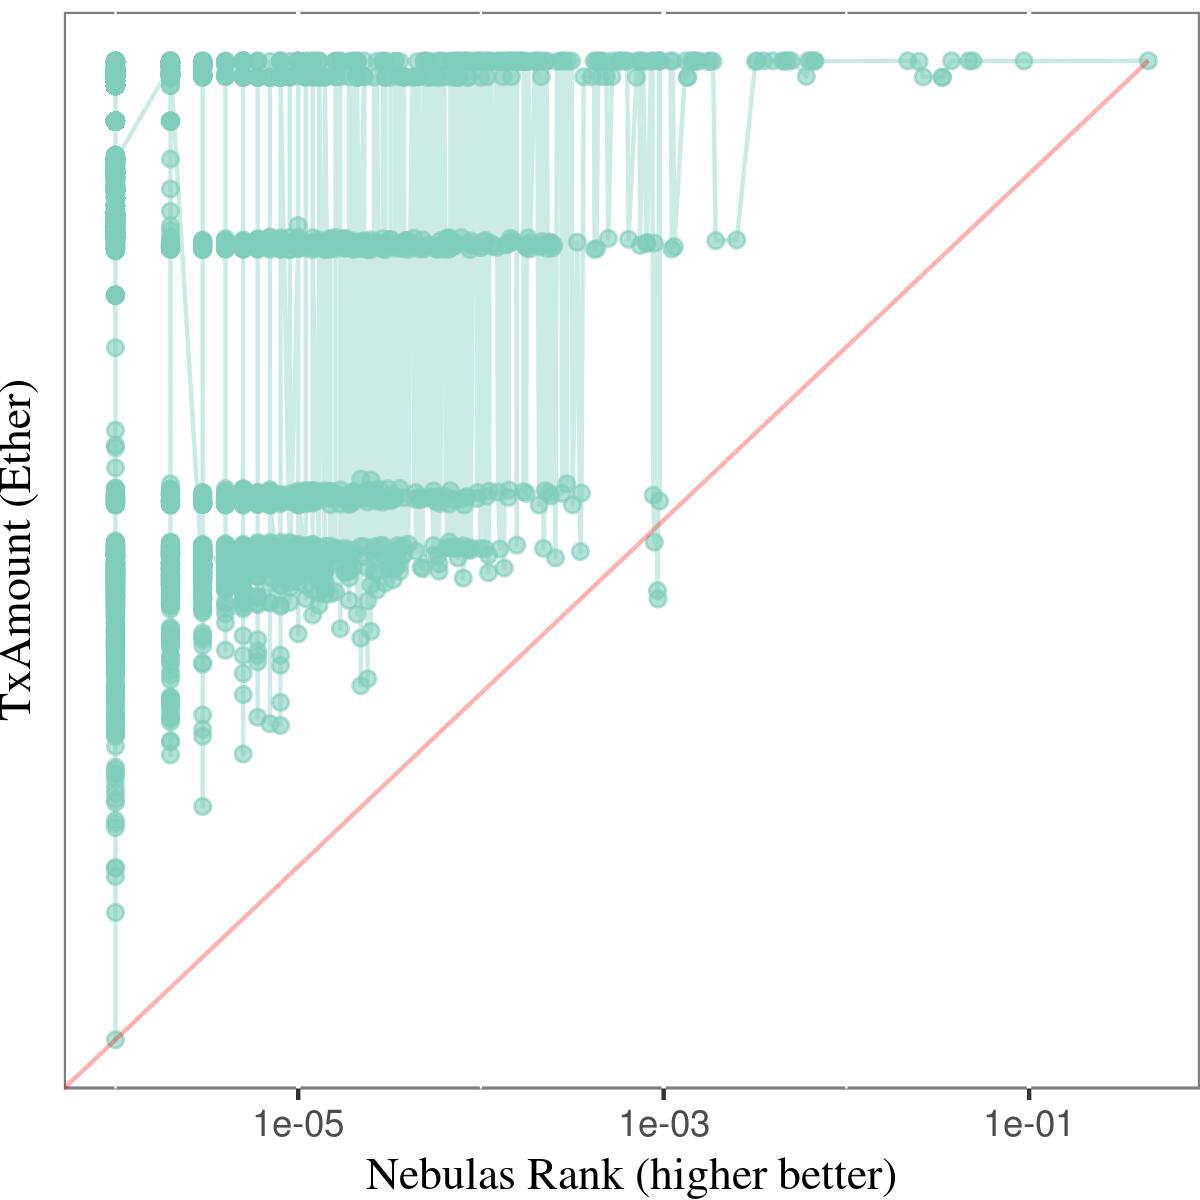
\includegraphics[width=0.50\textwidth]{figs/MAY_lr.png}
	\caption{Nebulas Rank v.s. Transaction Amount \small{X-axis represents Rank Value, and Y-axis represents Transaction Amount, both in logarithmic form.  The diagonal line represents that transaction amount and rank value is directly proportional. A good algorithm should make the data points fall as little as possible in the lower right of the diagonal line, to avoid nodes with low transaction throughput to get high rank.}}\label{fig:nrio}
\end{figure}

According to the above simple analysis, it can be deduced that the first three types of manipulation can be filtered effectively by specific methods. Therefore finally, we just need to simulate the last type and observe the resistance effect. The attacker chooses one authoritative Exchange node to create loop transfers for $X$ times. Every loop transfer contains 2 phases: first the attacker transfers $Y$ Ether to the Exchange through some newly created temporary address; then the attacker retrieves its money back from the Exchange through another address. The attacking topology and process is demonstrated in \reffig{fig:loop}. This type of attack exploits the fact that an Exchange service is willing to establish links with any nodes at a very low cost. Although normal nodes can also transfer with Exchange nodes frequently, but such attacking activities do not improve effective money liquidity and should be distinguished from normal activities.
\begin{figure}[!ht]
	\centering
	%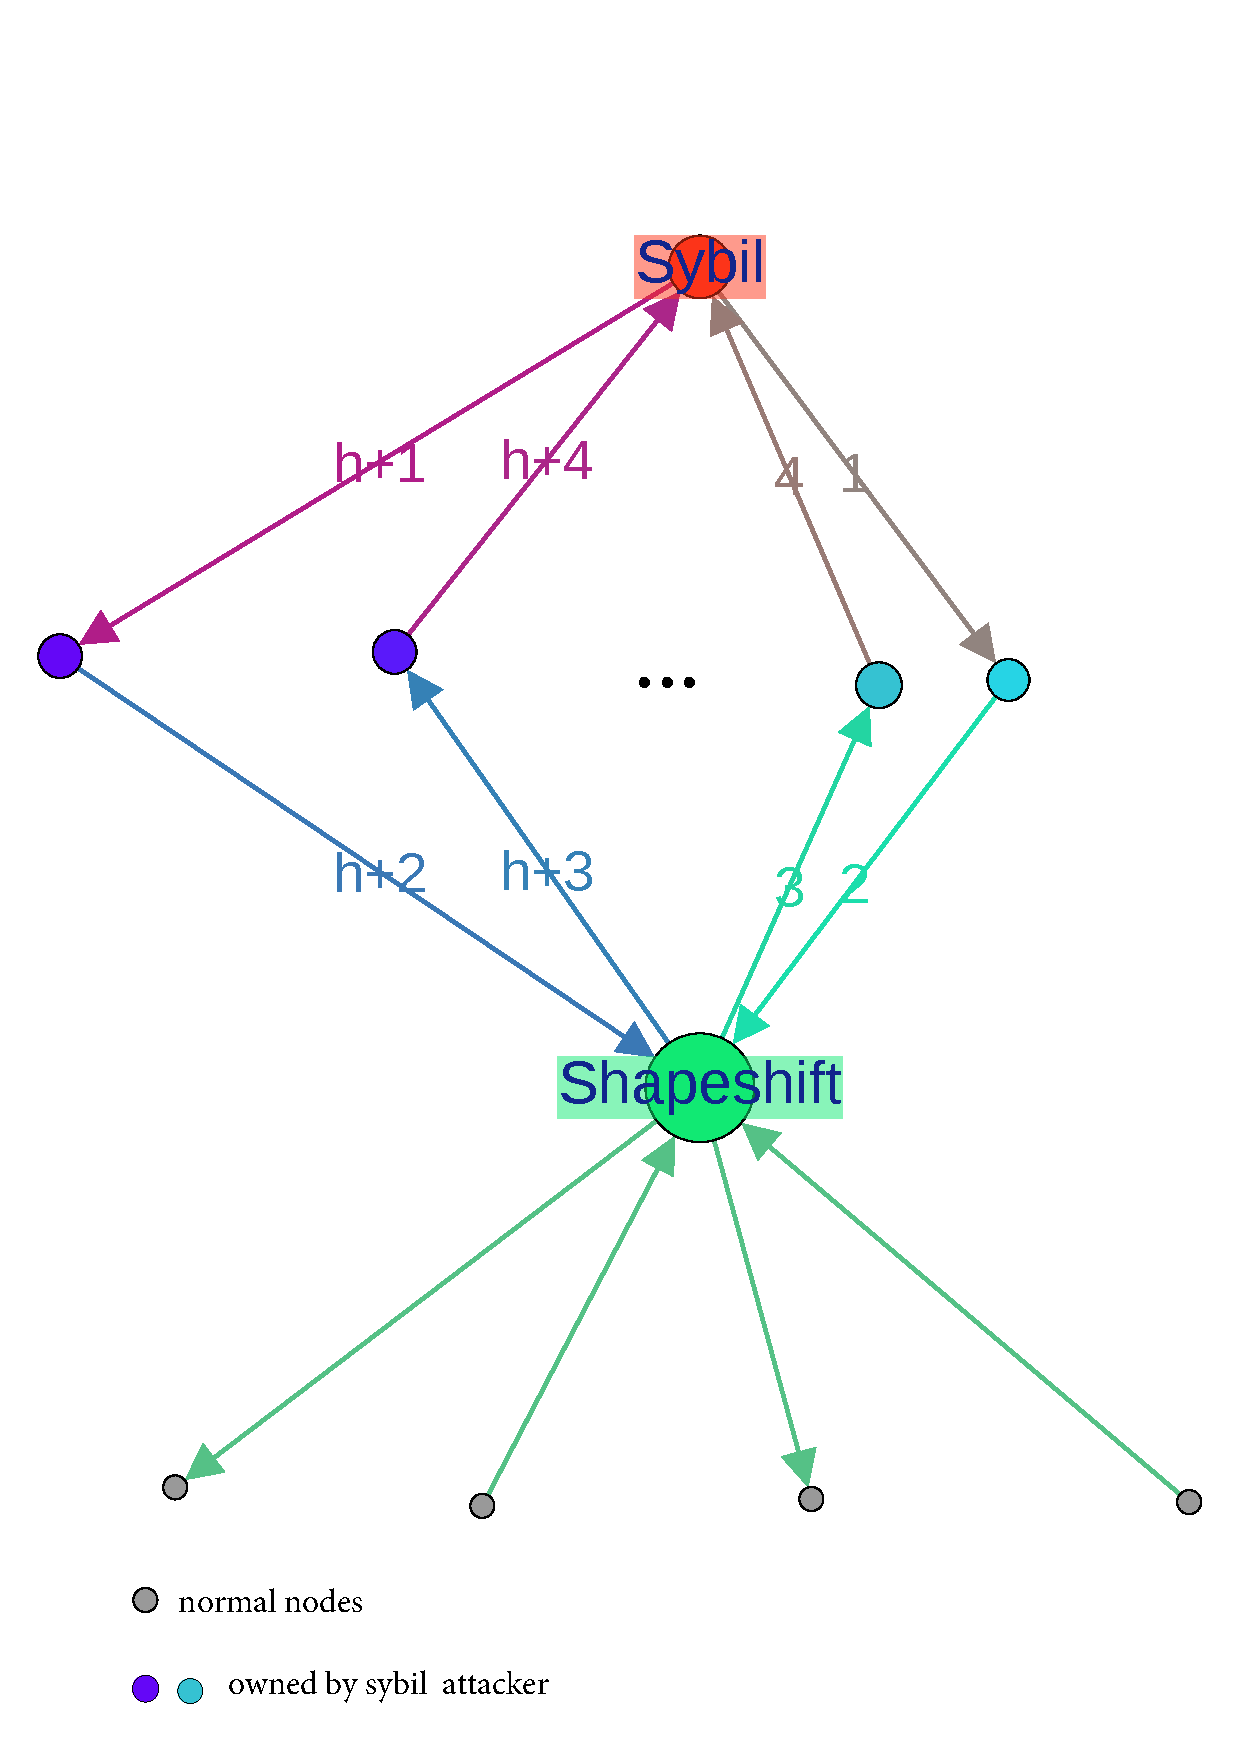
\includegraphics[width=0.35\textwidth]{figs/attack.pdf}
  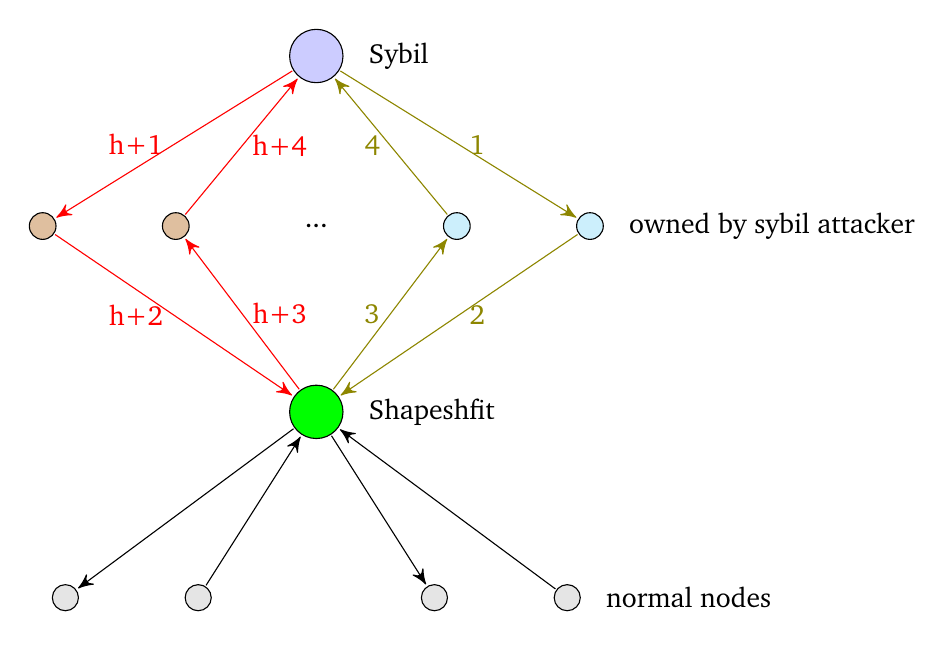
\begin{tikzpicture}
  \pgfmathsetmacro{\YMD}{2}
  \pgfmathsetmacro{\XMD}{1.5}
\tikzset{
  hnode/.style={draw, circle, on grid, align=center, minimum height=2ex},
  base/.style={draw, circle, on grid, align=center, minimum height=4ex},
  sybil/.style={draw, circle, on grid, align=center, minimum height=4ex, fill=blue!20},
  normal/.style={draw, circle, on grid, align=center, minimum height=1ex, fill=gray!20},
  coord/.style={coordinate, on grid, node distance=6mm and 25mm},
}
%
\tikzset{>=stealth',
  every join/.style={->}, very thick}

       \node [base, fill=green!=20] (ss) at (0, 0) {} node[right
       = 1ex of ss] {Shapeshfit};

       \node (dot) at ($(ss.north) + (0, \YMD)$) {...};

       \node [sybil] (sy) at ($(dot.north) + (0, \YMD)$) {} node[right=1ex of
       sy]{Sybil};

       \node [hnode, fill=brown!50] (hh4) at($(dot.west) + (-\XMD, 0)$){};
       \node [hnode, fill=brown!50] (hh1) at ($(hh4.west) + (-\XMD, 0)$){};

       \node [hnode, fill=cyan!20] (h4) at ($(dot.east) + (\XMD, 0)$){};
       \node [hnode, fill=cyan!20] (h1) at ($(h4.east) + (\XMD, 0)$){} node
       [right = 1ex of h1]{owned by sybil attacker};

       \node [coord] (c) at($(ss.south) + (0, -\YMD)$) {};

       \node [normal] (n2) at ($(c.west) + (-\XMD, 0)$){};
       \node [normal] (n1) at ($(n2.west) + (-\XMD, 0)$){};
       \node [normal] (n3) at ($(c.east) + (\XMD, 0)$){};
       \node [normal] (n4) at ($(n3.east) + (\XMD, 0)$){} node [right=1ex of
       n4] {normal nodes};

       \draw[->, color=red] (sy) -- (hh1) node [midway, left]{h+1};
       \draw[->, color=red] (hh4) -- (sy) node [midway, right]{h+4};
       \draw[->, color=olive] (h4) -- (sy) node [midway, left]{4};
       \draw[->, color=olive] (sy) -- (h1) node [midway, right]{1};

       \draw[->, color=red] (hh1) -- (ss) node [midway, left]{h+2};
       \draw[->, color=red] (ss) -- (hh4) node [midway, right]{h+3};
       \draw[->, color=olive] (ss) -- (h4) node [midway, left] {3};
       \draw[->, color=olive] (h1) -- (ss) node [midway, right]{2};

       \draw[->] (ss) -- (n1);
       \draw[->] (n2) -- (ss);
       \draw[->] (ss) -- (n3);
       \draw[->] (n4) -- (ss);

\end{tikzpicture}

	\caption{Schematic of Loop Attack Utilizing Exchange Address \small{The first and $h$-th loop attacks are shown in the figure. The selected authoritative Exchange node is Shapeshift; Edge label indicates temporal sequence; The transfer amount between nodes controlled by Sybil attacker and Shapeshift node is $Y$Ether; There are $X$ loop transfers during the manipulation.}}\label{fig:loop}
\end{figure}

We choose Shapeshift(0x70faa28a6b8d6829a4b1e649d26ec9a2a39ba413) as the authoritative Exchange address. The results is shown in \reffig{fig:antiManipulation}: 1) As is shown in \reffig{subfig:deposit}, with the attacker investing more capital, no algorithm is able to prevent the attacker's rank from being better, while the transaction graph defined in \refsec{subsec:txg} reduces the attacking effect. \textbf{Nebulas Rank} can not only prefer nodes with high transaction throughput, but also resist manipulation to some extent; 2) As is shown in \reffig{subfig:times}, with the attacker making more loop transfers, the transaction graph defined at \refsec{subsec:txg} can let the attacker's rank be worse. The reason is that such transaction graph considers factors like coinage and encouragement value. Meanwhile, \textbf{Nebulas Rank} could strengthen these factors, bringing more resistance against manipulation.

\begin{figure}[htbp]
	\centering
	\begin{subfigure}{\linewidth}
		\centering
		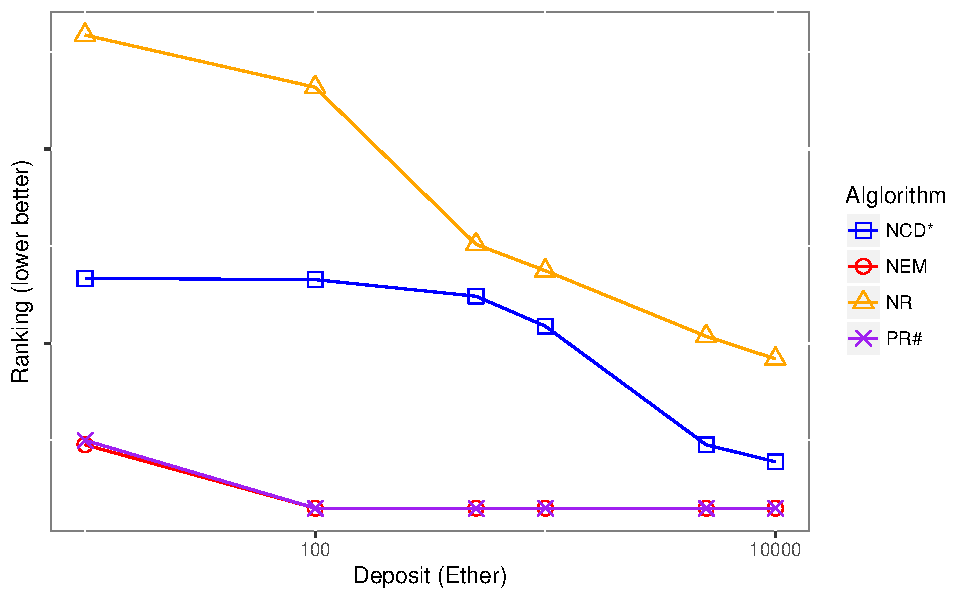
\includegraphics[width=0.7\textwidth]{figs/AttackDeposit.pdf}
		\caption{The effect of attacker's capital size on attacker's rank, with the number of loop transfers is fixed as $5,000$. \small{(All axises are in logarithmic form)}}
		\label{subfig:deposit}
	\end{subfigure}

	\begin{subfigure}{\linewidth}
	    \centering
		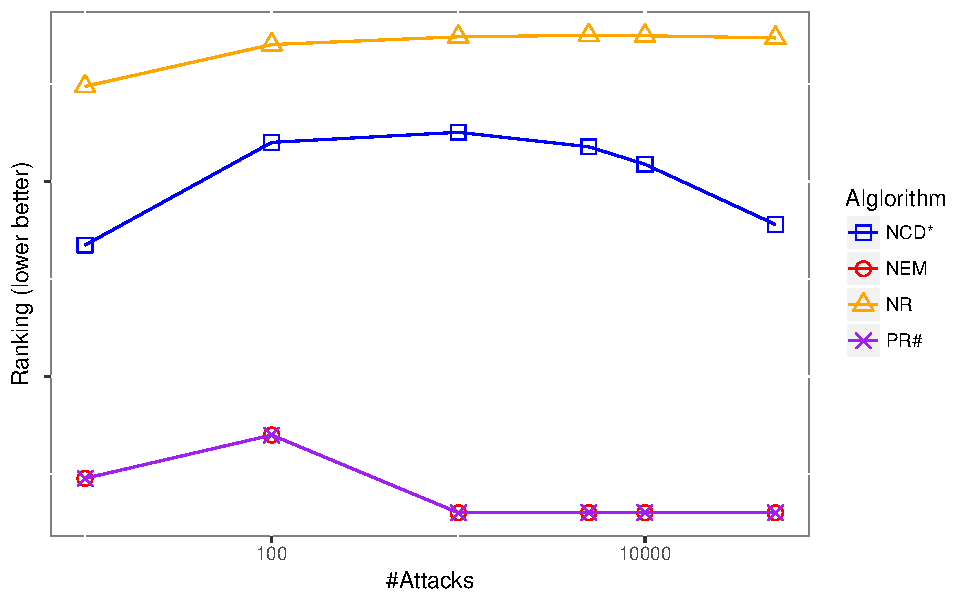
\includegraphics[width=0.7\textwidth]{figs/AttackTimes.pdf}
		\caption{The effect of number of loop transfers on the attacker's rank, with attacker's capital fixed as $\Xi5000$ \small{(All axises are in logarithmic form)}}\label{subfig:times}
	\end{subfigure}

	\caption{Resistance against manipulation} \label{fig:antiManipulation}
	\caption*{\footnotesize{The attacking method is shown as \reffig{fig:loop}; x-axis represents attacker's capital; y-axis represents attacker's ranking order (larger ranking order means the attacker fails to get better score, indicating higher resistance ability of the algorithm)  \\
	NR:The transaction graph is defined at \refsec{subsec:txg}, and ranking algorithm is described at \refsec{subsec:leaderrank}; \\
	%PR$^*$: The transaction graph is defined at \refsec{subsec:txg}, PageRank algorithm;\\
	NCD$^*$: The transaction graph is defined at \refsec{subsec:txg}, with NCDawareRank algorithm; \\
	NEM:The transaction graph is introduced by \cite{nem}, with NCDawareRank\\
	PR$^{\#}$: The transaction graph is introduced by \cite{nem},with PageRank algorithm\\
	The damping factor of PageRank is 0.15; The clustering algorithm used by NCDawareRank is pscan\cite{chang2017mathsf}, $\eta=0.75$, $\mu=0.1$}}
\end{figure}

\subsection{Related Works} \label{subsec:related}

Centrality, the core ranking index, is a most studied concept in network science since decades ago\cite{newman2010networks}. There are a body of literatures introducing various centralities, including degree centrality\cite{freeman1979set}, eigenvector centrality\cite{bonacich1972factoring}, Katz centrality\cite{katz1953new}, closeness centrality\cite{sabidussi1966centrality}, betweenness centrality\cite{freeman1977set}\cite{freeman1978centrality}\cite{freeman1991centrality}\cite{noh2004random}\cite{newman2005measure}, PageRank\cite{Brin2010}, HITS\cite{kleinberg1999authoritative}, SALSA\cite{Science2001}, etc. Besides, there are some fundamental works trying to clearly classify and review these measurements by a unified framework\cite{Borgatti2005}\cite{Borgatti2006}\cite{Lu2016}. When designing \textbf{Nebulas Rank}, before proper centrality is adopted, first we need to consider the property of graph. Blockchain transaction graph's scenario is most similar to the money exchange flow network mentioned in \cite{Borgatti2005}. But the related algorithms mentioned by their work, such as flow betweenness centrality\cite{freeman1991centrality} and random-walk betweenness centrality (aka. current betweenness centrality)\cite{newman2005measure}, are compute intensive and do not satisfy the property of ``computable" with the large scale of Blockchain transaction graph.

Since Bitcoin\cite{Nakamoto2008} system released in 2009, researchers have done some statistical and empirical analysis on Bitcoin's transaction graph\cite{Ron}\cite{Haslhofer}\cite{NielKondor2014}\cite{Baumann2014}, and some use the transaction graph structure to discuss anonymity in Bitcoin\cite{Meiklejohn2013}\cite{Ober2013}\cite{pham2016anomaly}\cite{Fleder2015}\cite{Ferrin2015}. After other cryptocurrencies emerged and become popular, transaction graph analysis is conducted for more blockchains\cite{Chang2017}\cite{Anderson2016}. \textbf{Nebulas Rank} adopts their transaction graph concept, i.e. Entity Graph in \cite{Tschorsch2015}, with minor revisions. That is, each account, or set of accounts belonging to the same people, is mapped as a node, and each directed edge represents the intensity of transferring between two accounts. Actually before blockchain system like Bitcoin was invented, scientists have tried to study some financial networks among banks and global trading entities\cite{propper2008towards}\cite{Boss2004}\cite{Serrano2007}\cite{Bech2008}\cite{Fagiolo2009}\cite{Morten2006}\cite{Boss2004a}\cite{Krempel2002}\cite{Serrano2003}. Comparing with blockchain transaction graph, these early studied finical networks are defined not only by transferring activities, but also by extra information such as loan. Moreover, the scale of these networks is much smaller. To conclude, there is rarely research work proposing custom ranking method for large scale transaction graph, especially blockchain transaction graph.

The most relevant work with \textbf{Nebulas Rank} is NEM\cite{nem}'s Proof-of-Importance scheme. It adopts NCDawareRank\cite{Nikolakopoulos2013}, which exploits the clustering effect of network topology, as the ranking algorithm, with clustering algorithm based on SCAN algorithm\cite{xu2007scan}\cite{shiokawa2015scan}\cite{chang2017mathsf}. Although community structure does exist in transaction graph and should be helpful to handle with spam nodes, it does not guarantee that all nodes in Blockchain world controlled by one entity in the real world are mapped into one cluster, which leads to large room for manipulation. Besides, \cite{Fleder2015} uses PageRank\cite{Brin2010}\cite{page1999pagerank} as an assisting metric to discover interesting addresses and analyze their activities. However, their work does not provide an automated framework to identify important nodes. Instead, it still relies on subjective analysis, which does not match \textbf{Nebulas Rank}'s context. The algorithm we choose is LeaderRank\cite{Chen2013}\cite{Li2014}. It is a simple yet effective variant of PageRank\cite{Brin2010}\cite{page1999pagerank}. In PageRank, every node is assigned with identical teleportation parameter, while LeaderRank adds a ground node, assigning different teleportation parameters for each node. The weighing scheme of \textbf{Nebulas Rank} is partly from \cite{Li2014}'s design, which allows nodes with more in-degree to be more likely visited by teleportation. Adopting LeaderRank algorithm could yield results more suitable for the scenario of Blockchain. %TRADUCIDO
\newpage
\section{Nebulas Force}
\label{sec:nebulasforce}

We use Nebulas Force (NF) to describe the evolutionary capability of the blockchain system and its applications. As the first driving force of the blockchain system and its application development, the Nebulas Force includes three aspects, that is, the Nebulas Virtual Machine (NVM), the upgrade of the core protocol in the blockchain system, and the upgrade of the smart contract running on the blockchain system.

%我们使用星云原力(Nebulas Force, NF)来描述区块链系统及应用的进化能力。星云原力做为驱动区块链系统及应用发展的第一推动力,包括三个方面:星云链虚拟机NVM(Nebulas Virtual Machine),区块链系统中核心协议的升级,以及运行在区块链系统之上的智能合约的升级。

In Nebulas, we will introduce LLVM to implement the Nebulas Virtual Machine (NVM). The core protocol and the smart contract code will be compiled into NVM bytecode, which is dynamically compiled and optimized with the LLVM just-in-time (JIT) compilation function and eventually executed in the sandbox environment. Meanwhile, with the modular architecture of LLVM, developers can use their familiar programming languages to implement safer and higher-performance smart contracts, providing users with various decentralized applications.

%在星云链中,我们将引入LLVM来实现星云链虚拟机NVM。核心协议和智能合约代码将会编译成NVM字节码,通过LLVM即时编译(Just-in-time compilation)功能,实现其动态编译和优化,最终在沙箱环境中执行。同时借助于LLVM的模块化架构,开发者可以用熟悉的编程语言实现更高性能和更安全的智能合约,给用户带来更丰富的去中心化应用。

For the upgrade of the core protocol in Nebulas, Nebulas will add the core protocol to block structure to carry out the upgrade of the core protocol by supplementing additional data on chains so as to avoid the possible split or bifurcation between developers and communities. With the development of Nebulas communities, the upgrade capability of NF and basic protocols will be gradually open to communities, and communities will define the evolutionary direction of the Nebulas and achieve its upgrade target. With the help of the core technology and the opening concept of NF, Nebulas will have a continuously evolutionary space and an infinitely evolutionary possibility. For example, a series of parameters including the NR algorithm parameter, the PoD incentive amount, the consensus algorithm and the production rate of new tokens can be gradually adjusted during the development of Nebulas without upgrading most client codes.

%对于星云链中的核心协议升级,星云链将核心协议加入到区块中,通过对链上数据的追加实现核心协议的升级,避免开发者和社区的分裂或分叉的可能性。随着星云链社区的发展,NF及基础协议升级能力将逐步开放给社区,由社区定义星云链的进化方向并实现其升级目标。借助于NF这个核心技术和开放性的理念,星云链将会具有持续的进化空间和无限的进化可能。例如,NR算法参数、PoD激励金额、共识算法及新代币的生产速度等一系列参数,都可以在星云链的发展过程中逐渐调整,而不需要大部分客户端代码的升级。

The smart contract is usually considered to be permanent and does not support upgrading. With the help of the design of underlying storage of the smart contract to support the cross-contract visit of state variables, Nebulas can complete the upgrade of the smart contract. This solution is very friendly to developers, making them respond to bugs more rapidly, which can prevent huge losses to users caused by any hacker events.

%智能合约通常被认为是永久性的,不支持升级。星云链通过在智能合约底层存储支持状态变量可跨合约访问的设计,完成智能合约的升级,这种解决方案对开发者友好,使得开发者面对漏洞,能够更快的响应和升级,避免黑客事件给用户带来巨大的损失。

\subsection{NVM 星云链虚拟机}
\label{sec:nvm}

我们将引入LLVM~\cite{llvm}做为NVM的核心组件,并使用LLVM Byte Code做为NVM字节码。NVM字节码通过LLVM JIT完成动态编译和优化,运行在NVM沙盒环境中。在这种架构设计下,星云链的核心代码、智能合约能直接享受到LLVM带来的性能和安全性的不断提升。

LLVM早期是Low Level Virtual
Machine的缩写,是一系列高度模块化的编译器和工具链技术的集合,包括Google、Apple在内的公司都使用它做为代码编译框架。LLVM提供了一套中立的中间表示(LLVM
IR)和相应的编译基础设施,并围绕这些设施提供了一套全新的编译策略,包括对LLVM
IR的优化、LLVM IR到不同硬件平台的代码生成、LLVM IR到LLVM Byte
Code的代码生成以及LLVM Byte Code在不同硬件平台上通过LLVM
JIT直接执行。如图\ref{fig:llvm}所示

%LLVM编译框架分为三层,第一层支持多种语言作为输入(例如C/C++,go和python等),第二层是一个共享式的优化器(对LLVM IR做优化处理),第三层是许多不同的目标平台(例如 Intel, ARM和PowerPC),如图\ref{fig:llvm}所示

\begin{figure}[h]
\centering
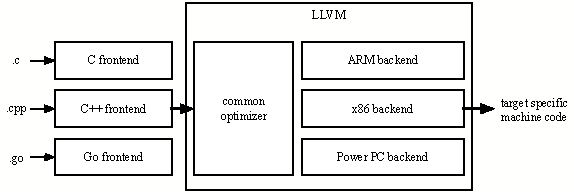
\includegraphics[width=10cm]{./figs/llvm}
\caption{LLVM}
\label{fig:llvm}
\end{figure}

我们依托LLVM构建NVM,如图\ref{fig:nvm}所示。首先,我们提供区块链底层API库;然后,我们为不同语言(如Solidity,JavaScript
,C/C++,Go等)构建生成LLVM
IR的编译器前端;最后,利用LLVM提供的工具链,生成LLVM Byte Code。最终,LLVM Byte
Code通过LLVM的JIT引擎运行在NVM提供的安全的沙箱环境中。
%然后,利用LLVM链接器链接我们提供的底层库,LLVM
%JIT完成核心协议和智能合约代码的编译、优化以及跨平台适配,生成机器代码;最后,让这些机器代码通过LLVM的JIT引擎运行在NVM提供的安全的沙箱环境中。

\begin{figure}[h]
\centering
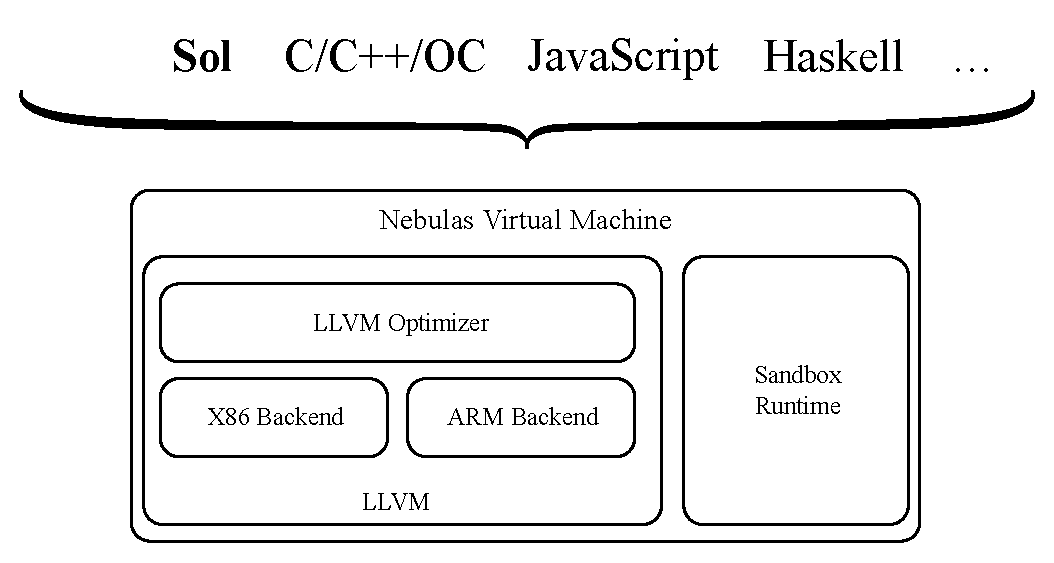
\includegraphics[width=10cm]{./figs/nvm}
\caption{星云链虚拟机}
\label{fig:nvm}
\end{figure}

NVM是星云原力的重要基石。新的协议代码或智能合约发布时,NVM中LLVM编译器模块完成新代码的编译得到LLVM字节码,然后发布到链上;链上确认后,新代码将由LLVM
JIT完成编译和优化,然后进入沙箱取代旧代码并被执行,过程如图\ref{fig:nvm-process}所示。 \\

\begin{figure}[h]
\centering
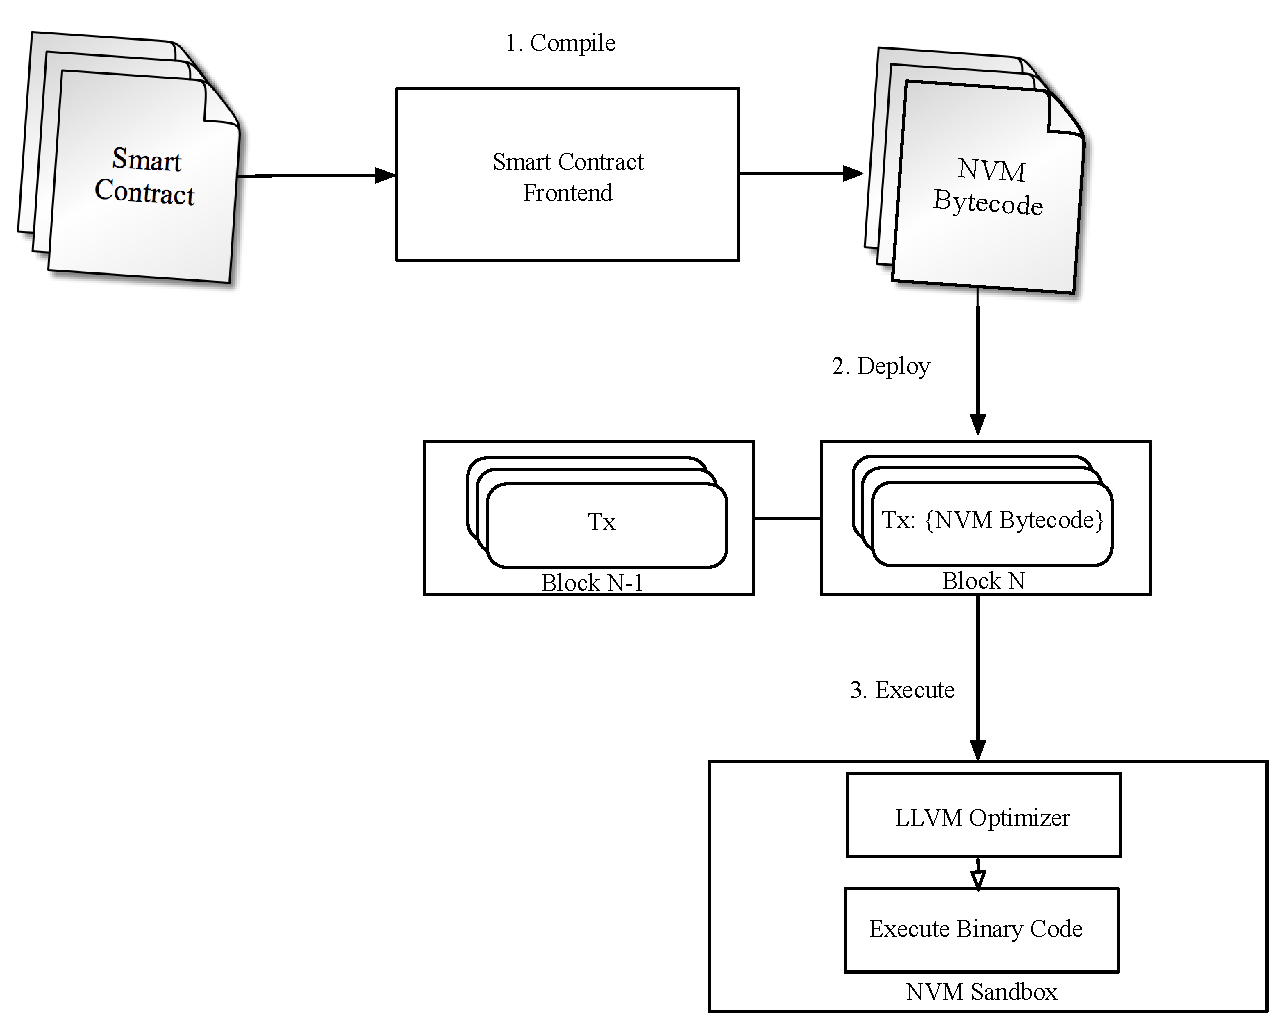
\includegraphics[width=10cm]{./figs/nvm-process}
\caption{星云链虚拟机运行机制}
\label{fig:nvm-process}
\end{figure}

借助于LLVM(见\ref{fig:llvm}),NVM还支持开发者用其熟悉的编程语言开发智能合约和应用,比如以太坊智能合约所使用的Solidity,更加灵活的JavaScript,甚至是纯函数式语言Haskell。除了这些通用语言外,NVM还可以为不同领域和场景提供定制的高级语言,比如面向金融行业的DSL(领域专有语言)。这类高级语言面向行业、场景高度定制,使得它们更容易被形式化验证,能进一步提高代码健壮性和安全性,更有利于星云链开发者开发出更丰富的智能合约及应用。

\subsection{核心协议的升级设计}

我们首先给出星云链中的区块结构,然后讨论如何在该区块结构上实现核心协议的升级问题。

\paragraph{区块结构}

星云链区块数据结构包含,但不限于以下信息:
\begin{itemize}
	\item Header:区块头
		\begin{itemize}
		\item Height:高度
		\item ParentHash:父区块哈希值
		\item Ts:时间戳
		\item Miner:记账人地址
		\item Dynasty:区块所处共识朝代
		\item Epoch:区块所处共识时代
		\item RankVer:区块所处NR周期
		\item RankRoot:区块所处NR周期的排名哈希值
		\item StateRoot:状态根哈希值
		\item TxsRoot:交易根哈希值
		\item ReceiptsRoot:交易收据根哈希值
		\item TransNum:交易数
		\end{itemize}
	\item Transactions:交易数据(包含多个交易)
		\begin{itemize}
		\item From:交易发起人地址
		\item To:交易接收人(普通用户或智能合约)地址,对于创建智能合约,值为0地址
		\item Value:转账金额
		\item Data:交易的payload。如果交易为创建智能合约,则为智能合约字节码;如果交易为智能合约调用,包含调用函数名称和入参值
		\item Signature:交易签名
		\item Gas:燃料上限
		\item GasPrice:燃料单价
		\item Nonce:标识交易唯一性
		\end{itemize}
	\item Votes:Prepare和Commit票数统计(包含多个),用在PoD(见\refsec{sec:pod})共识算法中
		\begin{itemize}
		\item From:投票人
		\item VoteHash:投票区块哈希
		\item Hv:投票区块所处高度
		\item Hvs:投票区块的某祖先高度
		\item VoteType:投票类型,Prepare或Commit
		\item Signature:投票签名
		\end{itemize}
	\item Protocol Code:核心协议代码(一个区块中只能有0或1个)
		\begin{itemize}
		\item Hash:哈希值
		\item Code:核心协议的字节码
		\item ValidStartBlock:协议生效起始区块号
		\item Signature:签名(校验是否来自开发者社区保留账号的签名)
		\item Version:标识核心协议版本号,每次升级都需要递增,防止恶意记账人回滚到老的Protocol Code
		\item Nonce:标识唯一性
		\end{itemize}
	\item Nebulas Rank:星云指数(计算周期为一周一次,大部分区块没有)
		\begin{itemize}
		\item Address:账号地址标记
		\item Score:NR值
		\end{itemize}
\end{itemize}

\begin{figure}[h]
\centering
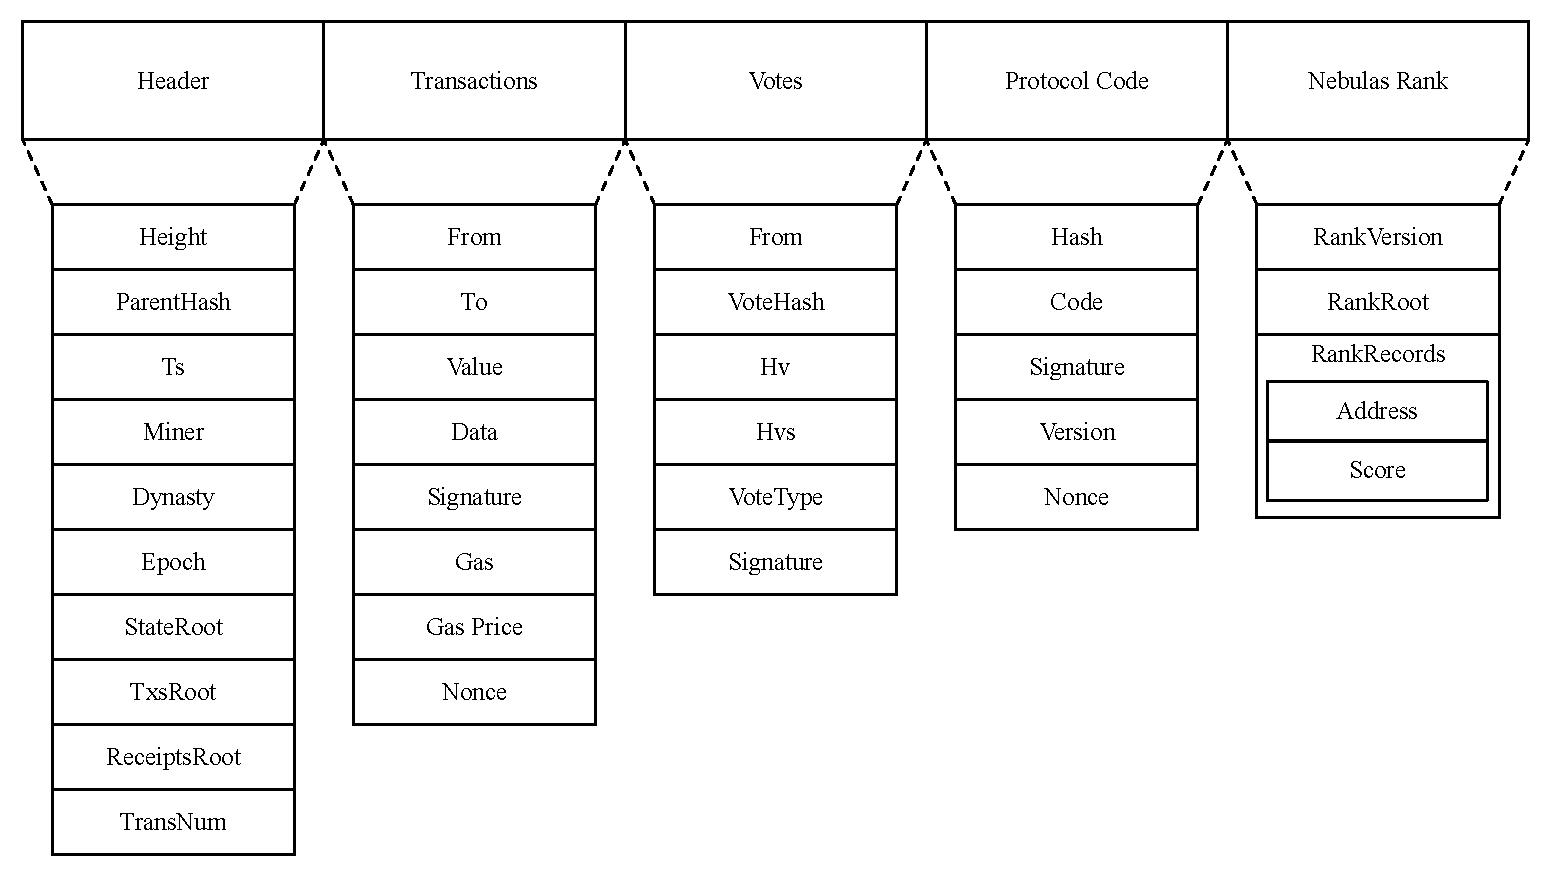
\includegraphics[width=13cm]{./figs/block}
\caption{区块结构}
\label{fig:block}
\end{figure}


类似于其他加密数字货币系统,用户和区块链上的互动都是通过特定的交易进行的。用户创建一笔交易,用自己的私钥签名后,发到区块链的任何一个节点中,通过P2P网络广播到全网节点。在固定的出块时间间隔内,由PoD共识算法(见\refsec{sec:pod})指定的记账节点累计这段时间内的所有交易,打包成标准格式的区块,同步到全网所有节点。经各节点独立验证后,加入本地账本,成为全球总账本的一部分。

以太坊中,交易分为两种类型:普通账户交易,智能合约交易。我们在星云链的区块中,增加新的数据类型:核心协议代码和星云指数。核心协议代码作为区块链数据的一部分存储在链上,星云链基础协议的升级,是通过链上数据的追加而实现的。星云指数根据NR排序算法,计算出每个周期各个账户的NR值存到链上,方便NR值的实时调用和历史排名查询。

\paragraph{核心协议的升级}

星云链客户端节点从当前最新区块的Protocol Code存储区可以取到编译后的虚拟机字节码(LLVM IR),如果当前最新区块没有Protocol Code数据,说明核心协议没有变更,就往前追溯到最近区块的Protocol Code。区块链的核心协议行为都由Protocol Code确定,包括验证算法、打包规则、NR算法、奖励机制等,几乎绝大部分的区块链行为都可以由Protocol Code定义。

如果核心协议需要升级,由星云链团队开发,把代码在公开渠道让社区讨论和投票。投票可以通过智能合约或者论坛投票的形式进行,当绝大部分社区成员都同意协议升级,星云链开发组把最新代码打包成Protocol Code交易,发布到全网节点,记账节点只要把其包含进区块,就可以在指定区块高度开始生效。这种方式的区块链协议升级,对客户端来说是透明的,无需软、硬分叉。

为了保证核心协议代码是经过授权发布的,Protocol Code的发布者是星云链核心开发组保留地址,该地址在创世区块内部硬编码无法变更。所有记账节点都会验证Protocol Code签名,签名不通过的视为非法数据。

后续的改进措施是把Protocol Code的签名校验改成M-of-N的多签名形式,这个本身也可以通过Protocol Code的升级实现。

\section{智能合约}

\subsection{图灵完备的智能合约编程语言}
智能合约是一套以数字形式定义的承诺(promises),包括合约参与方可以在上面执行这些承诺的协议。在物理上,智能合约的载体是计算机可识别并运行的计算机代码。比特币脚本语言是一种命令式的、基于栈的编程语言,由于它是非图灵完备的,所以应用上有一定的局限性。以太坊是全世界第一个实现图灵完备的智能合约的区块链系统,编程语言是Solidity、Surpent,使得应用开发者们可以高效快速地开发各式各样的应用程序。智能合约代码发布到区块链上之后,能够无需中介的参与,在区块链上自动执行。星云链中的智能合约编程语言,在初期时完全兼容以太坊的Solidity,方便开发者为以太坊开发的智能合约应用无缝的迁移到星云链中来。我们在Solidity语言中增加一些跟Nebulas Rank相关的指令集,方便开发者获取任意用户的NR值。后续我们会设计自己的智能合约二进制规范,推出各种编程语言的支持,使得开发者可以用自己喜欢的高级语言编程,例如Java、Python、Go、JavaScript、Scala等。

\subsection{合约可升级设计}
目前以太坊智能合约的设计是代码一经部署,不可变化,代码逻辑从部署的时刻起,便永远不再具有升级的能力。智能合约如果作为协议来看,不可变化是其要求的,代表着一种协议的约定,运行行为都是确定性的。但是随着智能合约开始获得越来越多的使用,其流程和代码也变得越来越复杂,人们发现,就像现实世界的合同一样,如果没有认真审核的话,在设计和编码过程中难以避免人工失误的产生,一旦被黑客找到漏洞,损失往往是巨大的。2016年6月,The DAO攻击事件,由于一个代码缺陷,导致以太坊用户损失了共计6000万美元的损失;最近Parity钱包的漏洞,导致15万个以太币的流失,价值3000万美元。比特币由于其设计上的非图灵完备性,删减了许多脚本指令,所以其安全性是极高的。

虽然目前有各种智能合约编程的最佳实践,以及更严格的审核流程,甚至出现形式化验证工具,通过数学证明的方式验证智能合约的确定性。但是既然是代码,就不可能没有漏洞。回顾我们现在的中心化的互联网世界,各种互联网服务都是可以升级的,弥补开发过程中发生的各种漏洞。任何一个完美的应用系统,都是演化而不是设计出来的。我们认为,解决智能合约安全性的根本问题,需要有一个好的智能合约可升级设计方案。

以太坊上的智能合约可升级设计有一些解决方案,大体上分为两类:一类是对外公开proxy contract(代理合约),代理合约的代码非常简单,仅仅把请求转发给后面的真正的功能合约。当需要升级合约时,把代理合约的内部功能合约指针指向新的合约即可;第二类是把合约的代码和存储分离,存储合约负责提供方法,供外部合约读写内部状态,代码合约做真正的业务逻辑,升级时只需要部署新的代码合约,不丢失所有的状态。这两类方案都有其局限性,不能解决所有问题:合约的代码和存储分离在设计上增加了很多复杂度,有时候甚至不可行;代理合约虽然能够指向新合约,但是老合约的状态数据并不能迁移;有些合约在开始开发时,没有良好的设计,没有为以后的升级留下接口。

我们设计一种简洁的智能合约升级方案:在语言层面上,我们支持一个合约的状态变量供另外一个合约直接读写(符合安全约束)。这是一个例子,假如有个Token合约,代码如下:
\begin{lstlisting}[frame=single]
contract Token {
  mapping (address => uint256) balances shared;

  function transfer(address _to, uint256 _value) returns (bool success) {
     if (balances[msg.sender] >= _value) {
       balances[msg.sender] -= _value;
       balances[_to] += _value;
       return true;
     } else {
       return false;
     }
   }
   function balanceOf(address _owner) constant returns (uint256 balance) {
       return balances[_owner];
   }
}
\end{lstlisting}

合约部署时,balances变量用关键字shared标识,编译成字节码运行时,虚拟机会为该变量单独设计存储区域。不用关键字shared声明的变量,都不可以被其它合约直接访问。

假如原代码的transfer函数需要修改一个bug,对\_value做检查,部署新的智能合约代码:

\begin{lstlisting}[frame=single]
[baseContractAddress="0x5d65d971895edc438f465c17db6992698a52318d"]
//baseContractAddress是老合约的地址
contract Token {
  mapping (address => uint256) balances shared;

  function transfer(address _to, uint256 _value) returns (bool success) {
     if (balances[msg.sender] >= _value && _value > 0) {
       balances[msg.sender] -= _value;
       balances[_to] += _value;
       return true;
     } else {
       return false;
     }
   }
   function balanceOf(address _owner) constant returns (uint256 balance) {
       return balances[_owner];
   }
}
\end{lstlisting}

新的合约部署以后,老的合约可以选择selfdestruct,不能再被访问,但是shared变量依然被永久保留。新的合约可以完全继承老合约的balances资产,全部的状态都不丢失,不需要做额外的迁移工作。但是在开发智能合约时,对关键的状态变量声明为shared是必须的,编译器会对变量的存储区域做特殊处理,保证其可以被其它授权的合约访问。

为了保证安全,升级合约和老合约必须是相同的creator,否则运行时会抛异常。

这种设计存在道德上的问题,因为合约的内容条款一旦拟订,其实是不应该被修改的,至少修改必须征询合约受众的同意。我们计划引入投票机制,以批准智能合约的升级,而不是默默的被合约创建者修改。

通过这种可升级方案,The DAO或者Parity类似的漏洞攻击事件,可以更快的被修复,而不是通过硬分叉的方式。并且修复以后,所有用户的资产都不需要迁移,仍然继续使用。



 %TRADUCIDO
\subsection{NVM 星云链虚拟机}
\label{sec:nvm}

我们将引入LLVM~\cite{llvm}做为NVM的核心组件,并使用LLVM Byte Code做为NVM字节码。NVM字节码通过LLVM JIT完成动态编译和优化,运行在NVM沙盒环境中。在这种架构设计下,星云链的核心代码、智能合约能直接享受到LLVM带来的性能和安全性的不断提升。

LLVM早期是Low Level Virtual
Machine的缩写,是一系列高度模块化的编译器和工具链技术的集合,包括Google、Apple在内的公司都使用它做为代码编译框架。LLVM提供了一套中立的中间表示(LLVM
IR)和相应的编译基础设施,并围绕这些设施提供了一套全新的编译策略,包括对LLVM
IR的优化、LLVM IR到不同硬件平台的代码生成、LLVM IR到LLVM Byte
Code的代码生成以及LLVM Byte Code在不同硬件平台上通过LLVM
JIT直接执行。如图\ref{fig:llvm}所示

%LLVM编译框架分为三层,第一层支持多种语言作为输入(例如C/C++,go和python等),第二层是一个共享式的优化器(对LLVM IR做优化处理),第三层是许多不同的目标平台(例如 Intel, ARM和PowerPC),如图\ref{fig:llvm}所示

\begin{figure}[h]
\centering
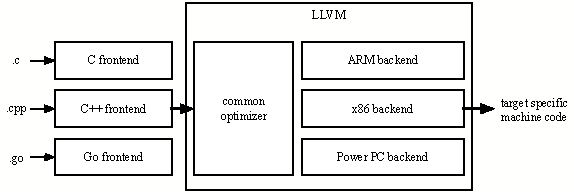
\includegraphics[width=10cm]{./figs/llvm}
\caption{LLVM}
\label{fig:llvm}
\end{figure}

我们依托LLVM构建NVM,如图\ref{fig:nvm}所示。首先,我们提供区块链底层API库;然后,我们为不同语言(如Solidity,JavaScript
,C/C++,Go等)构建生成LLVM
IR的编译器前端;最后,利用LLVM提供的工具链,生成LLVM Byte Code。最终,LLVM Byte
Code通过LLVM的JIT引擎运行在NVM提供的安全的沙箱环境中。
%然后,利用LLVM链接器链接我们提供的底层库,LLVM
%JIT完成核心协议和智能合约代码的编译、优化以及跨平台适配,生成机器代码;最后,让这些机器代码通过LLVM的JIT引擎运行在NVM提供的安全的沙箱环境中。

\begin{figure}[h]
\centering
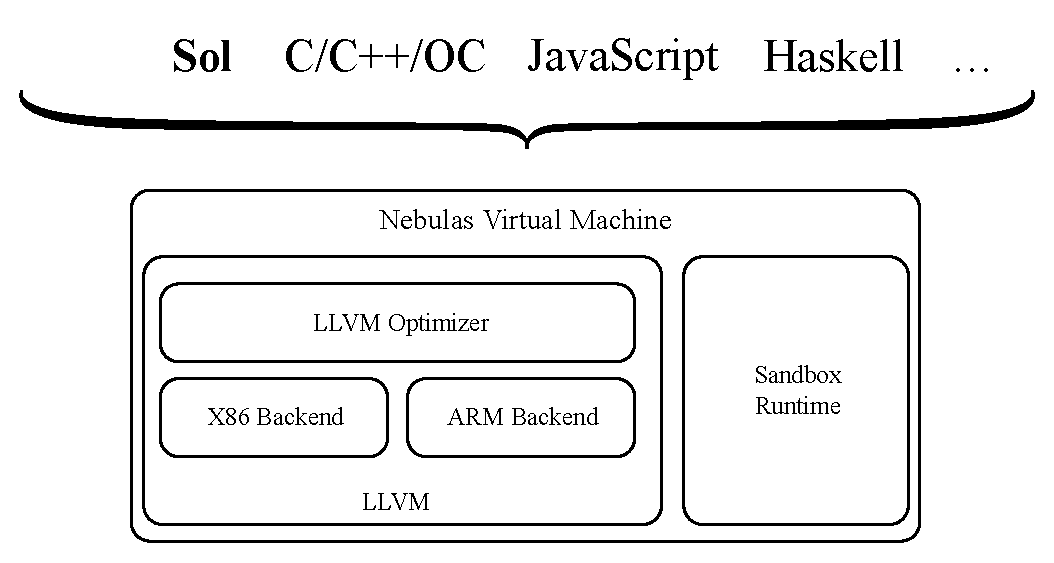
\includegraphics[width=10cm]{./figs/nvm}
\caption{星云链虚拟机}
\label{fig:nvm}
\end{figure}

NVM是星云原力的重要基石。新的协议代码或智能合约发布时,NVM中LLVM编译器模块完成新代码的编译得到LLVM字节码,然后发布到链上;链上确认后,新代码将由LLVM
JIT完成编译和优化,然后进入沙箱取代旧代码并被执行,过程如图\ref{fig:nvm-process}所示。 \\

\begin{figure}[h]
\centering
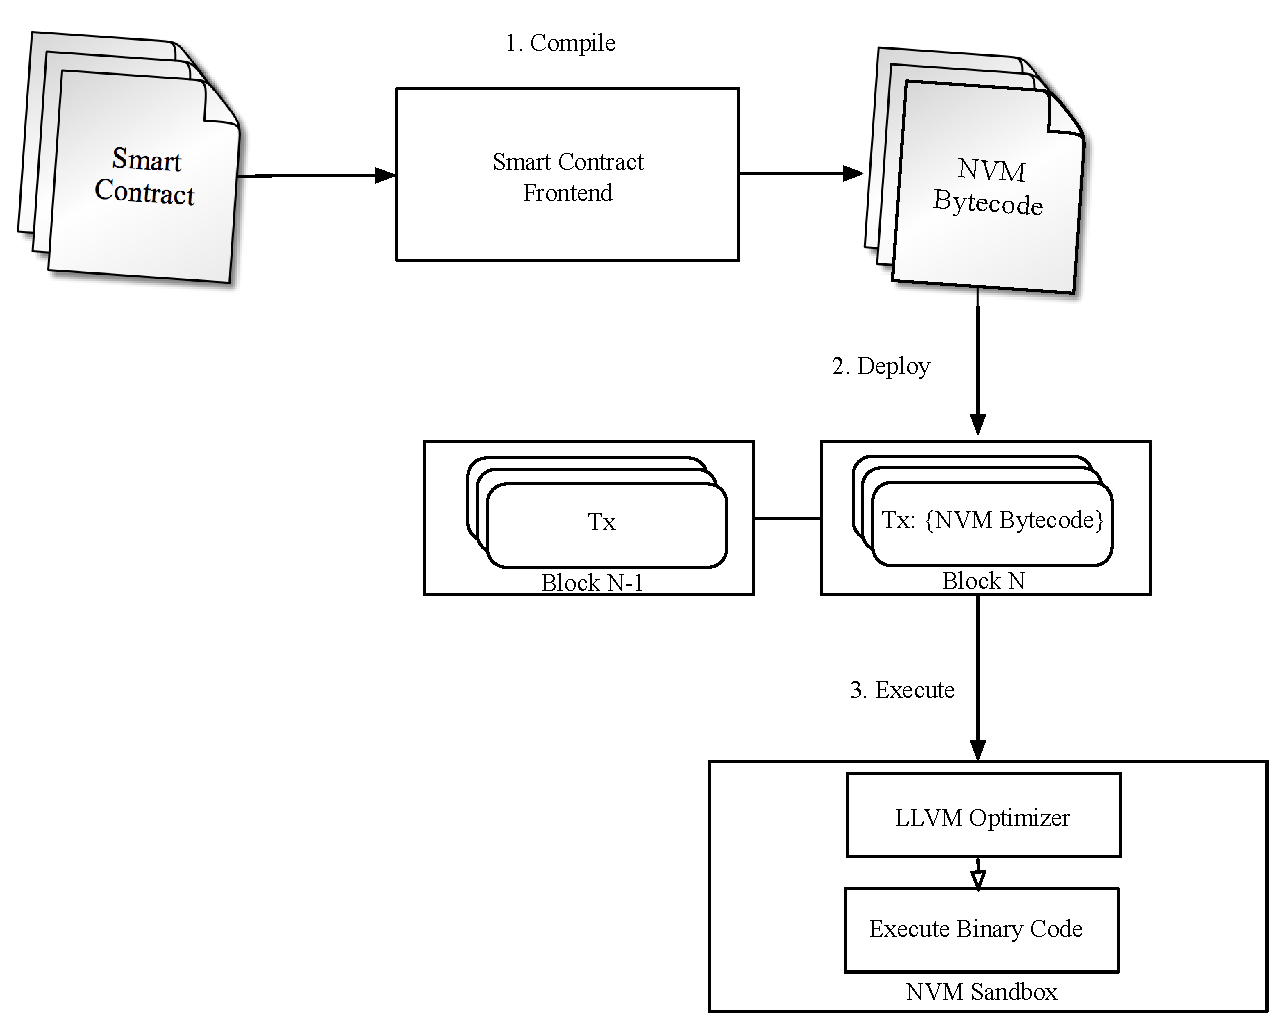
\includegraphics[width=10cm]{./figs/nvm-process}
\caption{星云链虚拟机运行机制}
\label{fig:nvm-process}
\end{figure}

借助于LLVM(见\ref{fig:llvm}),NVM还支持开发者用其熟悉的编程语言开发智能合约和应用,比如以太坊智能合约所使用的Solidity,更加灵活的JavaScript,甚至是纯函数式语言Haskell。除了这些通用语言外,NVM还可以为不同领域和场景提供定制的高级语言,比如面向金融行业的DSL(领域专有语言)。这类高级语言面向行业、场景高度定制,使得它们更容易被形式化验证,能进一步提高代码健壮性和安全性,更有利于星云链开发者开发出更丰富的智能合约及应用。
 %TRADUCIDO
\subsection{核心协议的升级设计}

我们首先给出星云链中的区块结构,然后讨论如何在该区块结构上实现核心协议的升级问题。

\paragraph{区块结构}

星云链区块数据结构包含,但不限于以下信息:
\begin{itemize}
	\item Header:区块头
		\begin{itemize}
		\item Height:高度
		\item ParentHash:父区块哈希值
		\item Ts:时间戳
		\item Miner:记账人地址
		\item Dynasty:区块所处共识朝代
		\item Epoch:区块所处共识时代
		\item RankVer:区块所处NR周期
		\item RankRoot:区块所处NR周期的排名哈希值
		\item StateRoot:状态根哈希值
		\item TxsRoot:交易根哈希值
		\item ReceiptsRoot:交易收据根哈希值
		\item TransNum:交易数
		\end{itemize}
	\item Transactions:交易数据(包含多个交易)
		\begin{itemize}
		\item From:交易发起人地址
		\item To:交易接收人(普通用户或智能合约)地址,对于创建智能合约,值为0地址
		\item Value:转账金额
		\item Data:交易的payload。如果交易为创建智能合约,则为智能合约字节码;如果交易为智能合约调用,包含调用函数名称和入参值
		\item Signature:交易签名
		\item Gas:燃料上限
		\item GasPrice:燃料单价
		\item Nonce:标识交易唯一性
		\end{itemize}
	\item Votes:Prepare和Commit票数统计(包含多个),用在PoD(见\refsec{sec:pod})共识算法中
		\begin{itemize}
		\item From:投票人
		\item VoteHash:投票区块哈希
		\item Hv:投票区块所处高度
		\item Hvs:投票区块的某祖先高度
		\item VoteType:投票类型,Prepare或Commit
		\item Signature:投票签名
		\end{itemize}
	\item Protocol Code:核心协议代码(一个区块中只能有0或1个)
		\begin{itemize}
		\item Hash:哈希值
		\item Code:核心协议的字节码
		\item ValidStartBlock:协议生效起始区块号
		\item Signature:签名(校验是否来自开发者社区保留账号的签名)
		\item Version:标识核心协议版本号,每次升级都需要递增,防止恶意记账人回滚到老的Protocol Code
		\item Nonce:标识唯一性
		\end{itemize}
	\item Nebulas Rank:星云指数(计算周期为一周一次,大部分区块没有)
		\begin{itemize}
		\item Address:账号地址标记
		\item Score:NR值
		\end{itemize}
\end{itemize}

\begin{figure}[h]
\centering
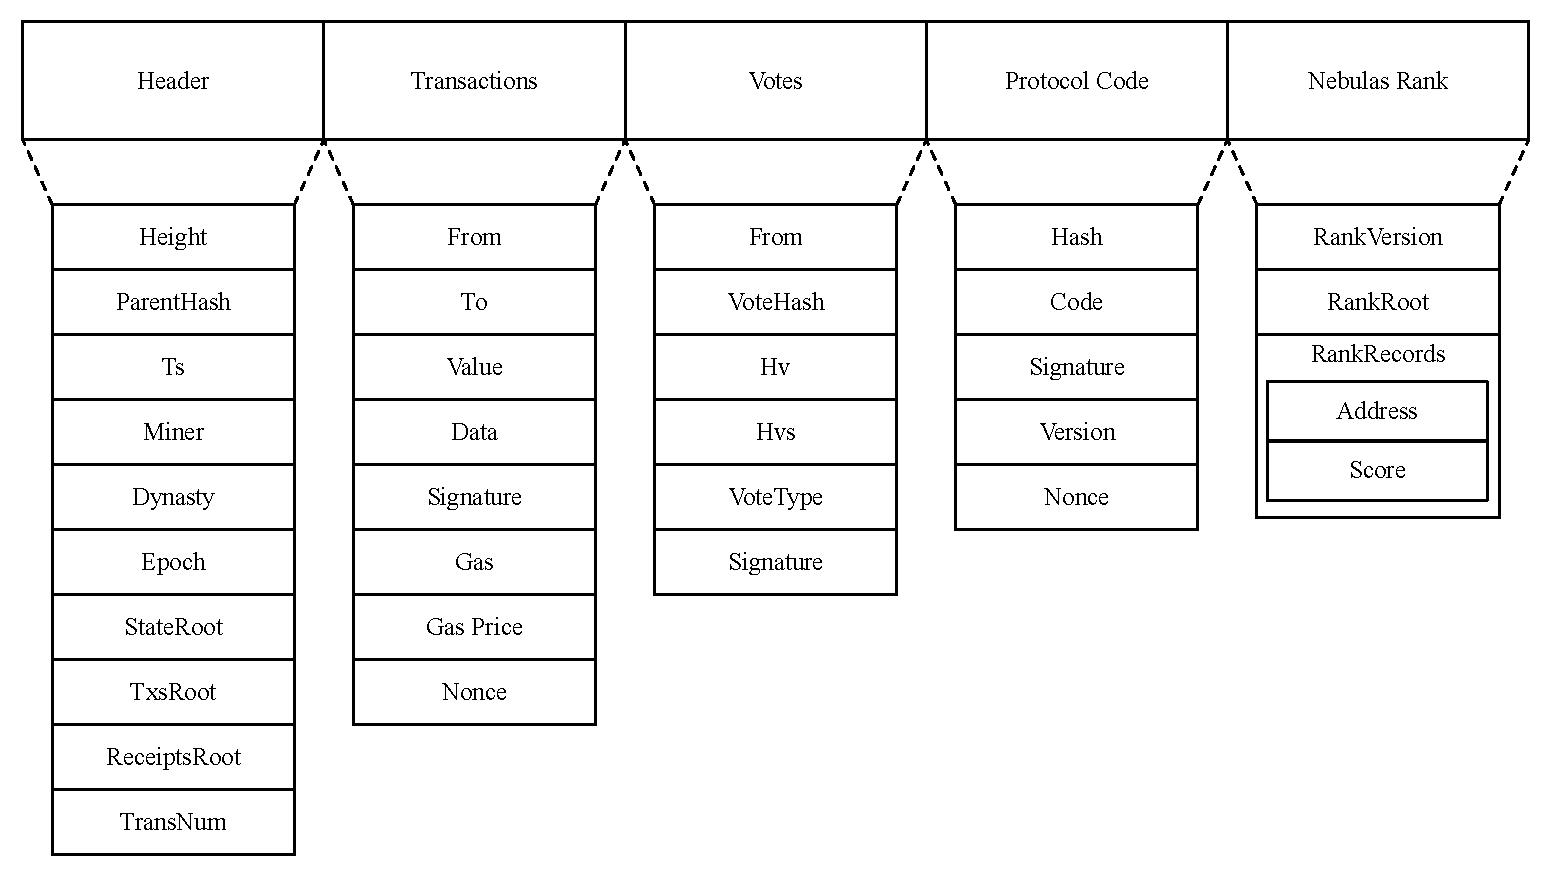
\includegraphics[width=13cm]{./figs/block}
\caption{区块结构}
\label{fig:block}
\end{figure}


类似于其他加密数字货币系统,用户和区块链上的互动都是通过特定的交易进行的。用户创建一笔交易,用自己的私钥签名后,发到区块链的任何一个节点中,通过P2P网络广播到全网节点。在固定的出块时间间隔内,由PoD共识算法(见\refsec{sec:pod})指定的记账节点累计这段时间内的所有交易,打包成标准格式的区块,同步到全网所有节点。经各节点独立验证后,加入本地账本,成为全球总账本的一部分。

以太坊中,交易分为两种类型:普通账户交易,智能合约交易。我们在星云链的区块中,增加新的数据类型:核心协议代码和星云指数。核心协议代码作为区块链数据的一部分存储在链上,星云链基础协议的升级,是通过链上数据的追加而实现的。星云指数根据NR排序算法,计算出每个周期各个账户的NR值存到链上,方便NR值的实时调用和历史排名查询。

\paragraph{核心协议的升级}

星云链客户端节点从当前最新区块的Protocol Code存储区可以取到编译后的虚拟机字节码(LLVM IR),如果当前最新区块没有Protocol Code数据,说明核心协议没有变更,就往前追溯到最近区块的Protocol Code。区块链的核心协议行为都由Protocol Code确定,包括验证算法、打包规则、NR算法、奖励机制等,几乎绝大部分的区块链行为都可以由Protocol Code定义。

如果核心协议需要升级,由星云链团队开发,把代码在公开渠道让社区讨论和投票。投票可以通过智能合约或者论坛投票的形式进行,当绝大部分社区成员都同意协议升级,星云链开发组把最新代码打包成Protocol Code交易,发布到全网节点,记账节点只要把其包含进区块,就可以在指定区块高度开始生效。这种方式的区块链协议升级,对客户端来说是透明的,无需软、硬分叉。

为了保证核心协议代码是经过授权发布的,Protocol Code的发布者是星云链核心开发组保留地址,该地址在创世区块内部硬编码无法变更。所有记账节点都会验证Protocol Code签名,签名不通过的视为非法数据。

后续的改进措施是把Protocol Code的签名校验改成M-of-N的多签名形式,这个本身也可以通过Protocol Code的升级实现。
 %TRADUCIDO
\section{智能合约}

\subsection{图灵完备的智能合约编程语言}
智能合约是一套以数字形式定义的承诺(promises),包括合约参与方可以在上面执行这些承诺的协议。在物理上,智能合约的载体是计算机可识别并运行的计算机代码。比特币脚本语言是一种命令式的、基于栈的编程语言,由于它是非图灵完备的,所以应用上有一定的局限性。以太坊是全世界第一个实现图灵完备的智能合约的区块链系统,编程语言是Solidity、Surpent,使得应用开发者们可以高效快速地开发各式各样的应用程序。智能合约代码发布到区块链上之后,能够无需中介的参与,在区块链上自动执行。星云链中的智能合约编程语言,在初期时完全兼容以太坊的Solidity,方便开发者为以太坊开发的智能合约应用无缝的迁移到星云链中来。我们在Solidity语言中增加一些跟Nebulas Rank相关的指令集,方便开发者获取任意用户的NR值。后续我们会设计自己的智能合约二进制规范,推出各种编程语言的支持,使得开发者可以用自己喜欢的高级语言编程,例如Java、Python、Go、JavaScript、Scala等。

\subsection{合约可升级设计}
目前以太坊智能合约的设计是代码一经部署,不可变化,代码逻辑从部署的时刻起,便永远不再具有升级的能力。智能合约如果作为协议来看,不可变化是其要求的,代表着一种协议的约定,运行行为都是确定性的。但是随着智能合约开始获得越来越多的使用,其流程和代码也变得越来越复杂,人们发现,就像现实世界的合同一样,如果没有认真审核的话,在设计和编码过程中难以避免人工失误的产生,一旦被黑客找到漏洞,损失往往是巨大的。2016年6月,The DAO攻击事件,由于一个代码缺陷,导致以太坊用户损失了共计6000万美元的损失;最近Parity钱包的漏洞,导致15万个以太币的流失,价值3000万美元。比特币由于其设计上的非图灵完备性,删减了许多脚本指令,所以其安全性是极高的。

虽然目前有各种智能合约编程的最佳实践,以及更严格的审核流程,甚至出现形式化验证工具,通过数学证明的方式验证智能合约的确定性。但是既然是代码,就不可能没有漏洞。回顾我们现在的中心化的互联网世界,各种互联网服务都是可以升级的,弥补开发过程中发生的各种漏洞。任何一个完美的应用系统,都是演化而不是设计出来的。我们认为,解决智能合约安全性的根本问题,需要有一个好的智能合约可升级设计方案。

以太坊上的智能合约可升级设计有一些解决方案,大体上分为两类:一类是对外公开proxy contract(代理合约),代理合约的代码非常简单,仅仅把请求转发给后面的真正的功能合约。当需要升级合约时,把代理合约的内部功能合约指针指向新的合约即可;第二类是把合约的代码和存储分离,存储合约负责提供方法,供外部合约读写内部状态,代码合约做真正的业务逻辑,升级时只需要部署新的代码合约,不丢失所有的状态。这两类方案都有其局限性,不能解决所有问题:合约的代码和存储分离在设计上增加了很多复杂度,有时候甚至不可行;代理合约虽然能够指向新合约,但是老合约的状态数据并不能迁移;有些合约在开始开发时,没有良好的设计,没有为以后的升级留下接口。

我们设计一种简洁的智能合约升级方案:在语言层面上,我们支持一个合约的状态变量供另外一个合约直接读写(符合安全约束)。这是一个例子,假如有个Token合约,代码如下:
\begin{lstlisting}[frame=single]
contract Token {
  mapping (address => uint256) balances shared;

  function transfer(address _to, uint256 _value) returns (bool success) {
     if (balances[msg.sender] >= _value) {
       balances[msg.sender] -= _value;
       balances[_to] += _value;
       return true;
     } else {
       return false;
     }
   }
   function balanceOf(address _owner) constant returns (uint256 balance) {
       return balances[_owner];
   }
}
\end{lstlisting}

合约部署时,balances变量用关键字shared标识,编译成字节码运行时,虚拟机会为该变量单独设计存储区域。不用关键字shared声明的变量,都不可以被其它合约直接访问。

假如原代码的transfer函数需要修改一个bug,对\_value做检查,部署新的智能合约代码:

\begin{lstlisting}[frame=single]
[baseContractAddress="0x5d65d971895edc438f465c17db6992698a52318d"]
//baseContractAddress是老合约的地址
contract Token {
  mapping (address => uint256) balances shared;

  function transfer(address _to, uint256 _value) returns (bool success) {
     if (balances[msg.sender] >= _value && _value > 0) {
       balances[msg.sender] -= _value;
       balances[_to] += _value;
       return true;
     } else {
       return false;
     }
   }
   function balanceOf(address _owner) constant returns (uint256 balance) {
       return balances[_owner];
   }
}
\end{lstlisting}

新的合约部署以后,老的合约可以选择selfdestruct,不能再被访问,但是shared变量依然被永久保留。新的合约可以完全继承老合约的balances资产,全部的状态都不丢失,不需要做额外的迁移工作。但是在开发智能合约时,对关键的状态变量声明为shared是必须的,编译器会对变量的存储区域做特殊处理,保证其可以被其它授权的合约访问。

为了保证安全,升级合约和老合约必须是相同的creator,否则运行时会抛异常。

这种设计存在道德上的问题,因为合约的内容条款一旦拟订,其实是不应该被修改的,至少修改必须征询合约受众的同意。我们计划引入投票机制,以批准智能合约的升级,而不是默默的被合约创建者修改。

通过这种可升级方案,The DAO或者Parity类似的漏洞攻击事件,可以更快的被修复,而不是通过硬分叉的方式。并且修复以后,所有用户的资产都不需要迁移,仍然继续使用。


 %TRADUCIDO
\newpage
\section{DIP开发者激励协议}
\label{sec:dip}

为了更好地建立区块链应用的生态环境,在星云链中,我们提出面向智能合约开发者的DIP(Developer Incentive Protocol,开发者激励协议),通过星云币的奖励来感谢为生态助力的优秀智能合约开发者。

我们认为,一个智能合约是否优秀取决于有多少用户愿意使用它,而且有更多的高价值账户使用的智能合约更加优秀,而作为账户普适价值尺度的NR正好可以应用在高价值账户的评估中。DIP的设计结合NR和常用的周活跃用户的概念,使用周活跃用户的价值尺度总和来衡量智能合约的价值尺度,然后使用该价值尺度来评估开发者的贡献度。DIP每周进行一次,和Nebulas Rank计算周期一致。对于智能合约C,假设本周活跃账户地址集合为WAA(Weekly Active Addresses),其中根据\refsec{sec:nrrank}的NR分数,计算周活跃地址的NR之和作为合约C的贡献度SCS(Smart Contract Score)。

\begin{align}
SCS(C)=\sum_{addr \in WAA}NR(addr)
\end{align}

按照每周贡献值SCS从高到低排序得到智能合约贡献度排名SCR(Smart Contract Rank),取Top N的智能合约,它们对应的开发者将按比例瓜分M个星云币作为奖励,为了避免恶意刷榜,DIP的分配曲线被设计得较为平均,如图\ref{fig:dip_dist}所示,但依旧保证Rank 1的收益为Rank N收益的一倍以示贡献度大小的区别,如公式\ref{formula:dip}所示。

\begin{alignat}{2}
Coin(C) = & \quad kln(N+1-SCR(C))+b \label{formula:dip} \\
\mbox{s.t.}\quad & kln(N) + b = 2b \nonumber \\
& \sum_{x=1}^{N}(kln(x) + b) = M \nonumber
\end{alignat}

\begin{figure}[h] 
\centering
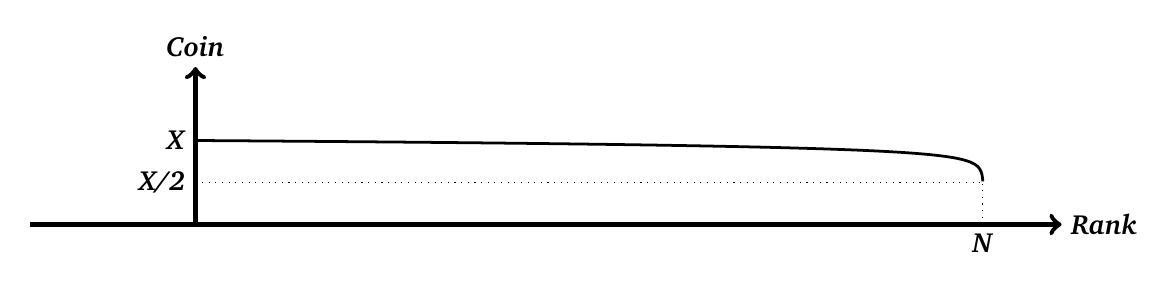
\begin{tikzpicture}
\coordinate (OR) at (0.00, 0.00);
\coordinate (LX) at (-2.10, 0.00); % left x
\coordinate (RX) at (11.00, 0.00); % right x
\coordinate (BY) at (0.00, 0.00); % bottom y
\coordinate (TY) at (0.00, 2.00); % top y
\draw[->][line width=1.75pt] (LX) -- (RX);
\node[right,black] at (11,0) {\textbf{\textit{Rank}}};
\draw[->][line width=1.75pt] (BY) -- (TY);
\node[above,black] at (0, 2) {\textbf{\textit{Coin}}};
\draw[dotted] (0,0.533210267)--(10,0.533210267);
\draw[dotted] (10,0)--(10,0.533210267);
\node[below,black] at (10, 0) {\textbf{\textit{N}}};
\node[left,black] at (0, 0.533210267) {\textbf{\textit{X/2}}};
\node[left,black] at (0, 1.066420536) {\textbf{\textit{X}}};
\draw[black, line width=1.00pt, domain=0:10.00,samples=3000] plot[smooth](\x, {.066598275 * ln(3001-\x * 300) + .533210267});

\end{tikzpicture}
\label{fig:dip_dist}
\caption{DIP奖励分配曲线}
\end{figure}

DIP的奖励将会由各个节点单独计算发放,假设星云链平均每S秒出一个区块,那么每隔24*7*3600/S个区块,所有节点将会计算一次DIP的奖励,并且发给对应的智能合约的提币地址中。

为了鼓励星云链生态智能合约的多样性,让更多新生开发者的优秀成果也能获得激励,DIP规定每个智能合约同一个版本最多可以接受K次奖励,当使用星云原力(见\refsec{sec:nebulasforce})对合约做版本更新后,新版本将可以再次接受最多K次奖励。DIP将会根据排名每次选出还可以接受奖励的Top N智能合约给予激励,助推区块链应用生态发展。
 %TRADUCIDO
\newpage
\section{PoD Consensus Algorithm}
\label{sec:pod}

\subsection{Design Goals}
\label{pod:goals}

The consensus algorithm is one of the cornerstones of blockchains, and its rapidity and irreversibility are our focus. In addition, in order to build a good ecology of Nebulas, we believe that fairness is equally important. If the big capital can easily gain power to control the block consensus in Nebulas, the interests of many developers and users will be damaged. It is difficult for an ecology which cannot guarantee the interests of contributors to create in-depth value, as it goes against the design principles of Nebulas. Thus, the consensus algorithm should be designed to ensure the rapidity and irreversibility first, on which basis we will pursue fairness as much as possible, so as to guarantee the interests of contributors in Nebulas.

%共识算法作为区块链的基石之一,快速和不可逆是我们重点关注的目标。除此之外,为了更好地建设公链生态,我们认为公平性同样重要,如果大资本可以轻松占据公链中区块共识的话语权,那么会有很多公链上的开发者和用户的利益无端受损,一个不能保障公链建设者利益的生态,很难沉淀出价值深度,和星云链设计原则相违背。所以我们在设计共识算法时,在优先保证快速和不可逆的情况下,将尽可能追求公平性,维护公链建设者的利益。

\subsection{Defects of Commonly Used Consensus Algorithms}
\label{pod:weakness}

We have tried to find suitable commonly used consensus algorithms that match with our design goals, but these algorithms cannot completely meet our requirements.

%我们试图在较为常用的共识算法中找到符合我们设计目标的选择,但是这些算法和我们的目标多少都有些差距。

The PoW (Proof of Work) consensus algorithm is a zero-sum game, which uses the competitive hash calculation to determine the bookkeeper, rendering a great amount of electric power in the whole ecology wasted in the competition when any blocks are fed out, and thus the mining cost is high and the speed is restricted. With the increase of nodes involved in mining, the probability of each node to obtain the bookkeeping right will be reduced, leading to a continuous rise in the cost of stable feed-out of blocks under the PoW protocol. The Bitcoin, which continues to increase the difficulty of mining, has to face the situation sooner or later where the mining machine cannot make ends meet, while Ethereum has long been considering the use of the new PoS consensus algorithm Casper \cite{casper} to gradually replace the current PoW consensus \cite{buterin2013ethereum}. It can be seen that in view of the mining speed and the economic cost, the PoW is not beneficial to the long-term rapid development of the ecology of Nebulas, which is against our ``rapid" goals.

%PoW (Proof of Work)工作量证明共识算法为零和博弈,采用竞争性哈希计算来确定记账人,导致了整个生态每次出块时都有大量电能在竞争中被无端消耗,挖矿成本高,而且速度受限。如果把公链参与者作为整体来看,随着参与挖矿的节点增加,每个节点获得记账权的概率将会减小,那么PoW协议下生态维持平稳出块的成本将会持续升高。不断增加挖矿难度的Bitcoin早晚需要面临矿机收益入不敷出的情形,而Ethereum则早已在考虑使用新的PoS共识算法Casper~\cite{casper}来逐步取代现阶段的PoW共识~\cite{buterin2013ethereum}。可见,从挖矿速度和经济成本角度,PoW都不利于公链生态的长期快速发展,和我们“快速”的目标不相符。

The PoS (Proof of Stake) consensus algorithm attempts to use the asset amount to replace the hash rate and distribute the probability of obtaining the bookkeeping right according to the coin age or deposit amount. Currently, both Peercoin \cite{king2012peercoin} and the Casper Protocol of Ethereum adopt the PoS consensus algorithm. This algorithm overcomes the shortcoming of the high power consumption of PoW but visually enlarges the impact of the capital on the probability distribution of the bookkeeping right. Compared with PoW, the big capital under PoS is more likely to gain power to control the ecology and form large group monopoly, possibly damaging the interests of the ecology contributors and impacting adversely on the value generation of Nebulas, all of which are against our ``fairness" goal.

%PoS (Proof of Stake)股权证明共识算法试图采用资产的多寡来取代算力的作用,按照币龄或者押金数额来分配获得记账权的概率,现阶段Peercoin~\cite{king2012peercoin}和Ethereum的Casper协议都采用了PoS共识算法。这种算法解决了PoW高能耗的弊端,但很直观地放大了资本对记账权概率分配的影响,相较于PoW,在PoS下大资本更容易占据生态的话语权,形成大集团垄断,可能会对生态的建设者的利益造成损害,不利于公链生态的价值沉淀,同样和我们“公平性”的目标不相符。

The PoI (Proof of Importance) consensus algorithm was first proposed by Nem \cite{nem}. Different from PoS, the concept of account importance is introduced to PoI, and the account importance score is used to distribute the probability of the bookkeeping right. This algorithm overcomes the shortcoming of the high power consumption of PoW and relieves the PoS capital monopoly crisis, but exposes the ``nothing-at-stake" problem. The cost for a cheater to reverse a block is significantly reduced, which goes against our ``irreversibility" goal.

%PoI (Proof of Importance)重要度证明共识算法最早由Nem提出~\cite{nem},不同于PoS,PoI中引入了账户重要程度的概念,使用账户重要性评分来分配记账权的概率。这种算法解决了PoW的高能耗弊端,减缓了PoS的资本垄断危机,但暴露了nothing-at-stake的问题,作弊者逆转一个区块的成本被大大降低,和我们“不可逆”的目标不相符。

In short, in view of the discrepancy between commonly used consensus algorithms and our goals, we have proposed the PoD (Proof of Devotion) algorithm to integrate PoI, which evaluates the comprehensive account influence, with PoS, which involves strict economic penalties. PoS enhances the irreversibility of PoI, while PoI reversely contains the monopoly of PoS, which facilitates the free and rapid development of the ecology.

%综上,鉴于常用共识算法和我们目标存在差距,我们提出了基于账户贡献度的PoD (Proof of Devotion)算法,将评估账户综合影响力的PoI和具有严格经济惩罚的PoS相融合,利用PoS强化PoI的不可逆性,使用PoI反向遏制了PoS的垄断性,以此为生态自由快速发展助力。

\subsection{Design of the PoD Algorithm}
\label{pod:design}

\subsubsection{Generation of New Blocks}
\label{pod:design:block}

Similar to the PoI consensus algorithm that selects highly important accounts, the PoD selects the accounts with high influence in the ecology. The difference lies in that the PoD empowers the selected accounts to have the bookkeeping right with equal probability to participate in new block generation in order to prevent tilted probability that may bring about monopoly.

%类似PoI共识算法选取重要性高的账户,PoD将选取生态中贡献度较高的账户,不同之处在于,PoD赋予选取出来的账户平等概率的记账权来参与产生新区块 (block),防止概率倾斜衍生垄断。

When selecting accounts with high influence, we use NR, the universal measure of value generated from Nebulas. In the algorithm design of NR, we highlighted the liquidity and propagation of accounts (see \refsec{subsec:value}). We believe that the accounts featured with these properties have a high influence with regard to the ecology construction. Thus, in the PoD, the accounts ranked Top N in the NR will be selected, and after these accounts voluntarily pay a certain number of NASs as the deposit, they will be qualified as the validator of new blocks to participate in bookkeeping.

%在选择贡献度较高的账户时,我们使用了星云链原生的NR普适价值尺度评估。在NR的算法设计中,着重考虑了账户的流动性和传播性(见\refsec{subsec:value}),我们认为满足这些性质的账户对生态建设贡献度较高。所以在PoD中,将选取NR排名Top N的账户,这些账户自愿缴纳一定数量的Nas作为押金后则有资格成为新区块的验证者 (validator),参与记账。

After the validator set is provided, the PoD algorithm uses the pseudo-random number to determine which one in the set is the new block proposer, which need to pack recent transactions to generate the new block. The validator set is changeable. The eligible account can choose to join or quit the set. Besides, the eligible accounts may vary with the periodical change of NR. Therefore, we designed the dynamic validator set change mechanism in the PoD to implement the change of the validator set.

%在给定验证者集合 (validators set)之后,PoD算法通过伪随机数来决定验证者集合中谁是新的区块的提议者 (proposer),提议者产生新区块。验证者集合不是固定不变的,有资格的账户可以选择加入或者退出验证者集合,而随着周期性NR的变化,有资格的账户也会不一样。所以我们在PoD设计了验证者集合动态变化机制,来实现验证者集合的更迭。

\subsubsection{Dynamic Validators Set}
\label{pod:design:validators}

The validator set changes the same way as a dynasty, so the set is divided into different dynasties, and the validator set within a dynasty will not change. A dynasty cannot experience too rapid change, and no change should be made within a period of time. Thus, we define every X blocks as an Epoch, and in the same Epoch, no change takes place in the dynasty. Therefore, the change of dynasties will only occur when one Epoch is handed over to another. At that time, the first block of the previous Epoch will be investigated. If this block reaches the finality state, then the current Epoch will enter into the next dynasty of D1; otherwise, the previous dynasty of D0 will remain; the process of which is shown in \reffig{fig:epoch}.

%验证者集合的更迭就如朝代变更一样,于是我们将验证者集合按照朝代(dynasty)做划分,一个朝代内验证者集合不会发生变化。一个朝代不能更迭地过快,至少要保持一段时间不做变更,因此我们将每X个区块定义为一个Epoch,在同一个Epoch中朝代不会发生变化。所以朝代的变更只会发生在Epoch交接时,在此时将会考察上一个Epoch的第一个区块,如果此区块到达了finality状态,那么当前Epoch进入下一个朝代D1,否则延续上一个朝代D0不变,如图\ref{fig:epoch}所示。

\begin{figure}[h]
\centering
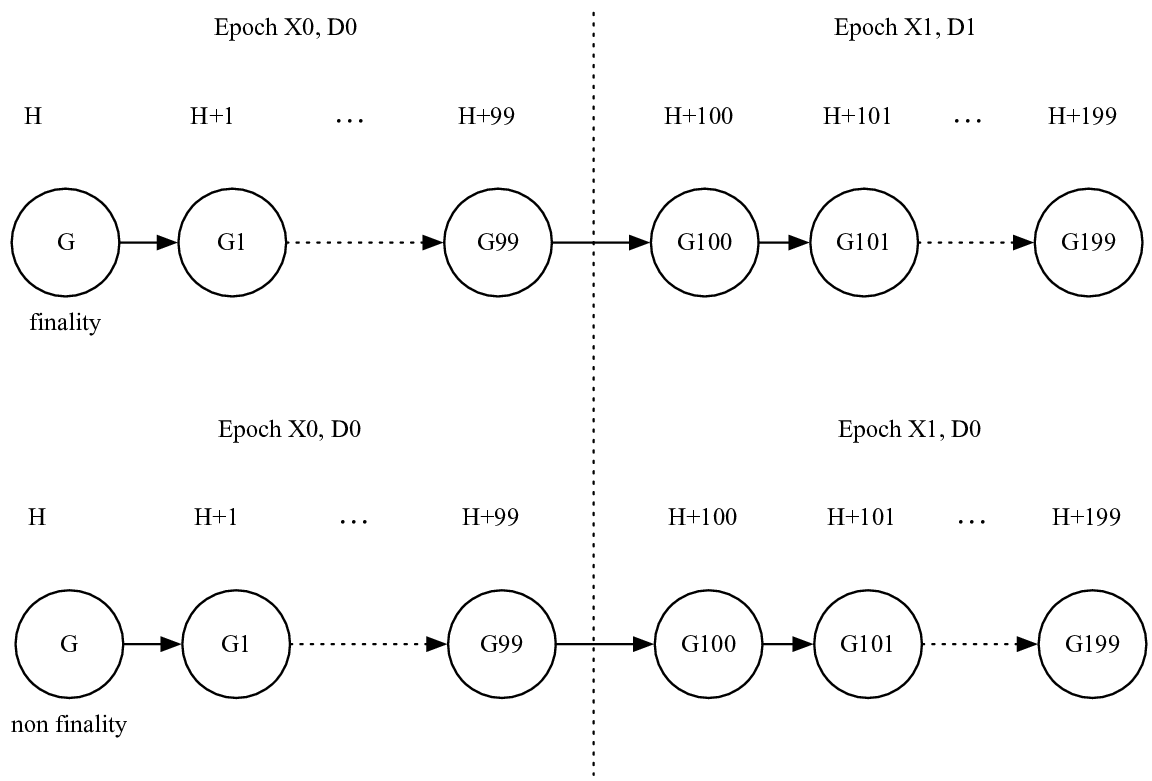
\includegraphics[width=8cm]{./figs/epoch}
\caption{Change of validator dynasties (assuming X = 100)}
\label{fig:epoch}
\end{figure}

Because of the network delay, the finality state of Block G at each node may not be the same when any change of dynasties takes place. Therefore, by reference to dynamic Casper validator set strategies, it is required that the consensus process of each dynasty will be completed jointly by the validator sets of the current and previous dynasties. Therefore, in any dynasty, an eligible account can only apply for joining or quiting the validator set of Dynasty D+2, and when the dynasty evolves into Dynasty D+2, it can participate in the consensus process of the new block.

%由于网络延迟,各个节点可能在朝代更迭时,看到的区块G是否finality的状态不一致,所以参考Casper的动态验证集策略,要求每一个朝代的共识过程将由当前朝代和上一个朝代的验证者集合共同完成。因此在任意一个朝代,有资格的账户只能申请加入或者退出D+2朝代的验证者集合,当朝代变更到D+2时,才可加入新区块的共识过程。

\subsubsection{Consensus Process}
\label{pod:design:consensus}

After a new block is proposed, all the people in the validator set of the current dynasty will participate in a round of BFT-Style (Byzantine-Fault-Tolerant Style) voting to determine the legitimacy of this block. In the beginning of voting, each validator who participates in this block consensus will be charged 2x (x is the incentive bonus proportion) as the deposit and then the two-stage voting process will be kicked off.

%新的区块被提出后,当前朝代验证者集合中所有人将会参与一轮BFT (Byzantine Fault Tolerant)方式的投票,来确定此区块的合法性。在投票最开始,每一个参与此区块共识的验证者将会被从押金中收取$2x$ ($x$为激励奖金比例)的保证金,然后进入两阶段的投票过程。

\begin{itemize}

\item \textbf{In the first stage}, it is required that all validators vote $Prepare$ tickets for the new block. After voting the $Prepare$ ticket, the validator will be rewarded $1.5x$ bonus. If the validators holding over two-thirds of the total deposits in both current and previous dynasties vote $Prepare$ tickets for the new block, this block will enter into the second stage of voting. It should be noted that the proposer of the new block votes the $Prepare$ ticket for the new block by default.

%\item \textbf{第一阶段},所有验证者需要对新区块投$Prepare$票,投完$Prepare$票的验证者将获得$1.5x$的奖励,如果在当前朝代和上一个朝代中都有超过$2/3$的押金总额的验证者对新区块投了$Prepare$票,那么该区块进入投票的第二阶段。此处需要说明,新区块的提议者将被默认对新区块投$Prepare$票。

\item \textbf{In the second stage}, it is required that all validators vote $Commit$ tickets for the new block. After voting the $Commit$ ticket, the validator will be rewarded $1.5x$ bonus again. If the validators holding over two-thirds of the total deposits in both current and previous dynasties vote $Commit$ tickets for the new block, this block will reach the finality state.

%\item \textbf{第二阶段},所有验证者需要对新区块投$Commit$票,投完$Commit$票的验证者,可以再获得$1.5x$的奖励,如果在当前朝代和上一个朝代中都有超过$2/3$的押金总额的验证者对新区块投了$Commit$票,那么该区块到达finality状态。
\end{itemize}

In order to speed up the development of the entire ecology, if the difference between the timestamp of $Prepare$ ticket and $Commit$ ticket in Block b and the timestamp of Block b exceeds $T$, then these tickets will be considered expired and will be ignored directly.

%为了加速整个生态向前延展,如果区块b的$Prepare$和$Commit$票的时间戳和区块b的时间戳相差超过T,那么这些票将被视为过期,直接忽略。

\subsubsection{Fork Choice}
\label{pod:design:fork}

The PoD algorithm selects the canonical chain according to the block score at each height. It always selects the block with the highest score to join the canonical chain, and the score of Block b at Height h is as follows:

%PoD算法以每个高度上区块的得分来选择权威链,总是选择得分最高的区块加入权威链,在高度h的区块b的得分如下,

\begin{align}
Score(b, h) = \sum_{(b',h') \in children(b)}Score(b', h') + \sum committed~deposits~in~b
\end{align}
\noindent 

Namely the sum of deposits corresponding to $Commit$ tickets received by this block and all of its descendant blocks, as shown in \reffig{fig:fork_choice}.

%即为该区块及其所有后代区块收到的commit票对应的押金总和,如图\ref{fig:fork_choice}所示。

\begin{figure}[h]
\centering
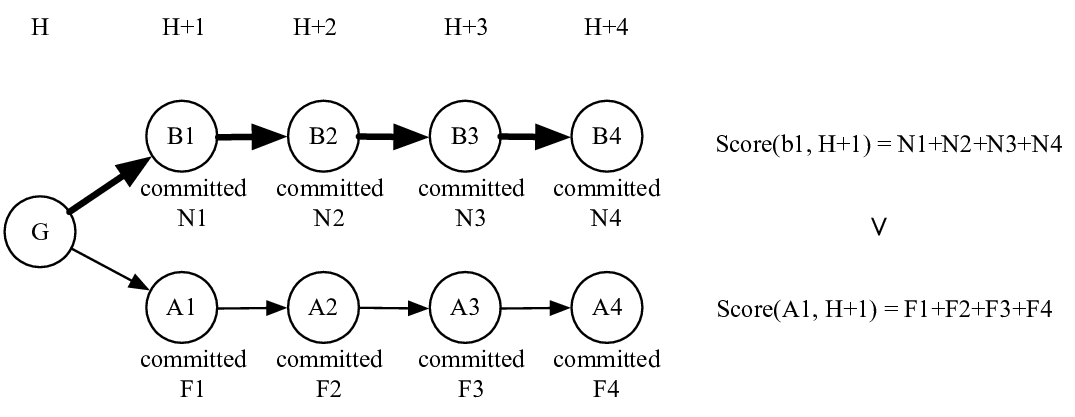
\includegraphics[width=12cm]{./figs/fork}
\caption{Fork Choice Example}
\label{fig:fork_choice}
\end{figure}

\subsubsection{Slashing Conditions}
\label{pod:design:vote}

To avoid any malicious damage to the consensus process, which may result in failure in the completion of consensus process and obstruction of eco-development, PoD constrains consensus activities of validators based on reference to Casper’s minimum slashing conditions \cite{minimal_slash_rules}.

%为了避免共识过程被恶意破坏,导致共识过程没法完成,阻碍生态发展,PoD参考Casper的最小惩罚规则~\cite{minimal_slash_rules}来约束验证者的共识活动。

Assume that $Prepare$ vote and $Commit$ vote in the consensus process have the following structures:

%假设共识过程中的$Prepare$和$Commit$票结构如下,

\begin{itemize}
\item $Prepare(H, v, vs)$, where $H$ is the hash value of the current block; $v$ represents the height of the current block; $vs$ represents the height of a certain ancestral block of $v$. 
%\item $Prepare(H, v, vs)$,其中$H$为当前区块hash,$v$表示当前区块高度,$vs$表示$v$的某个祖先区块高度

\item $Commit(H, v)$, where $H$ is the hash value of the current block; $v$ represents the height of the current block.
%\item $Commit(H, v)$,其中H为当前区块hash,$v$表示当前区块高度
\end{itemize}

PoD algorithm defines the following 4 basic rules for the entire voting process: 
%PoD算法为整个投票过程制定了如下4条基本规则,

\begin{itemize}
\item There is a strict order in the two-stage consensus process of a single block: Only when the total deposits of $Prepare(H, v, vs)$ votes for the first stage reaches $2/3$, can validators deliver $Commit(H, v)$ votes for the second stage.
%\item 单个区块的两阶段共识过程存在严格的先后顺序,只有在第一阶段$Prepare(H, v, vs)$票总权值达到$2/3$后,验证者们才可以投出第二阶段的$Commit(H, v)$票,

\item For multiple blocks, there is no mandatory rule that only when the consensus process of one block is finished, may consensus process of the next block begin. Interwoven consensus is permitted providing that it is conducted based on a certain order. Only after the first stage of process for height vs is finished and the proportion of $Prepare(H, vs, vs’)$ votes reaches $2/3$, can $Prepare(H, v, vs)$ votes for its descendant blocks be delivered based on vs in order to ensure stable proceeding of the interwoven consensus.
%\item 多区块间不强制一个区块共识结束后才能开始后一个区块的共识,允许交织共识(interwoven consensus),但是不能完全没有秩序,只有高度vs完成了第一阶段过程,拥有$2/3$的$Prepare(H_anc, vs, vs’)$后,才可以基于vs对其后代区块投$Prepare(H, v, vs)$票,保证交织稳步向前

\item To avoid the conduct of malicious cross-block voting of any node by taking advantage of the interwoven consensus, it is required that after the delivery of Prepare (H, w, u) votes based on the height of u, no Commit(H, v) vote can be delivered in all blocks with a height within the range from u to w, thus guaranteeing high efficiency and orderliness of the consensus process.
%\item 为了避免有节点利用交织共识恶意跨多区块投票,要求基于高度u投出了$Prepare(H, w, u)$票之后,对于高度在跨度u和w之间的所有区块,不能再投出$Commit(H, v)$票,保证共识过程的高效有序

\item For the purpose of preventing nodes from staking with one deposit on multiple branches simultaneously, which may lead to the problem of “nothing-at-stake”, it is required that after $Prepare(H1, v, vs1)$ votes are delivered at a certain height, no different $Prepare(H2, v, vs2)$ vote can be delivered again.
%\item 为了制止节点用同一笔押金在多个分支上同时下注,导致nothing~at~stake的问题,要求在一个高度投出$Prepare(H1, v, vs1)$票之后,不能再投出不一样的$Prepare(H2, v, vs2)$票
\end{itemize}

Once being reported and verified, any validators breaking the above rules will be punished and all his/her deposit will be confiscated, in which 4\% will be shared by whistleblowers as a reward and the remaining part will be destroyed.
%违反上述规则的验证者一旦被举报核实,将会被罚掉所有押金,举报者们将会共享罚金的4\%作为奖励,罚金的剩余部分将会被销毁。

\subsection{PoD Economic Analysis}
\label{pod:economic}

\subsubsection{Incentive Analysis}
\label{pod:economic:incentive}

A validator participating in the PoD algorithm will be rewarded with $1x$ NAS on each legal block. In case of failure in finishing the $Prepare$ stage and entering into the $Commit$ stage due to poor network traffic or any cheating behavior, the validator will lose $0.5x$ NAS. Therefore, any validator becoming value nodes will secure a large amount of earnings from accounting under good network traffic when not engaging in any cheating behavior.

%参与PoD算法的验证者,在每一个合法区块上可以获得1x的星云币奖励,如果网络不畅或者有人作弊导致Prepare阶段没有办法完成进入Commit阶段,那么所有验证者将损失0.5x。因此成为验证者的价值节点在保持网络畅通,不参与作弊的情况下,将共享大量记账收益。

\subsubsection{Cheating Analysis}
\label{pod:economic:fraud}

\subsubsection*{Double-spend Attack}
\label{pod:economic:fraud:double_spend}

If it is assumed that a merchant confirms transaction and makes delivery when the new block reaches the status of finality, then the minimum cost to be paid by a fraud for realizing zero-cost shopping through completion of double-spend attack under the PoD consensus algorithm is described as follows:

%假设商户merchant等到新区块到达finality状态就确认交易发货,那么fraud要在PoD共识算法下完成双重支付攻击实现零成本购物要付出的最小代价如下:

Firstly, the fraud needs to increase his/her Nebulas Rank to Top N, become a validator by paying a certain amount of NAS as deposit and apply for participation in validation of blocks in the D+2 dynasty. 

%首先,fraud需要提高自己的Nebulas Rank到Top N,然后缴一定数的NaS作为押金成为验证者,并申请参与D+2朝代区块的验证。

Then, the fraud needs to be selected as the proposer of a new block by the pseudo-random algorithm. At this moment, the fraud proposes two new blocks at the same height, of which one block has a hash value of hash1 and contains a transferring transaction from the fraud to the merchant, while the other block has a hash value of hash2 and contains a transferring transaction from the fraud to himself/herself. 

%然后,fraud需要被伪随机算法选中为新区块的提议者,此时fraud提出两个高度相同的新区块,一个哈希值为hash1包含fraud向merchant的转账交易,另一个哈希值为hash2包含fraud向fraud自己的转账交易。

Finally, in order to make both of hash1 and hash2 blocks reach finality, as shown in \reffig{fig:double_spend}, the fraud has to spend $1/3$ of the total deposits in this dynasty to bribe $1/3$ of the validators and make them to deliver $Commit$ votes to both blocks.

%最后,为了让hash1和hash2区块都到达finality,如图\ref{fig:double_spend}所示,fraud至少需要花费所有押金的$1/3$来贿赂$1/3$的验证者,让他们给两个区块都投$Commit$票。

\begin{figure}[h]
\centering
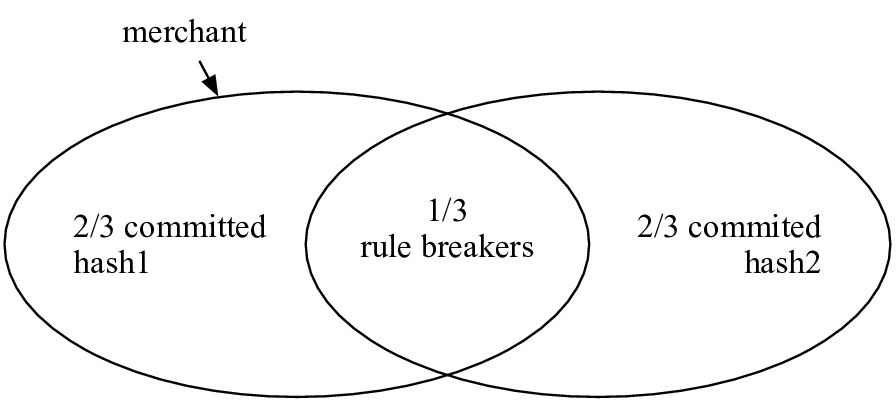
\includegraphics[width=7cm]{./figs/overlap}
\caption{Financial Punishment on Double Spend}
\label{fig:double_spend}
\end{figure}

Therefore, in order to complete a successful double-spend attack, the fraud needs to spend a certain amount of energy and financial resource to increase his/her Nebulas Rank (see \refsec{subsec:robust} Resistance to Manipulation) and then spend at least $1/3$ of the total deposits in current dynasty to make both of the blocks reach the finality status after he/she is luckily selected as a proposer.

%所以要完成一次成功的双重支付攻击,fraud需要花费一定的精力和财力来提升自己的Nebulas Rank排名(见\refsec{subsec:robust}抵抗操纵),然后等到幸运地被选为提议者时,至少花费总押金的$1/3$来让两个块同时到达finality状态。

\subsubsection*{51\% attack}
\label{pod:economic:fraud:51attack}

In PoW, launch of a 51\% attack requires 51\% of hashrate. In PoS, launch of a 51\% attack requires 51\% of deposit. However, in PoD, launch of a 51\% attack requires 51\% of accounts in the validators set, which means that a sufficient number of highly-reputed users need to rank at Top N in the Nebulas Rank and payment of a corresponding amount of deposit is required, so it will be more difficult to launch a 51\% attack in PoD.

%在PoW中要发起51\%攻击需要51\%的算力,在PoS中则需要51\%的押金,而在PoD中,则需要验证者集合中51\%的账户,这意味着拥有足够多的高声望用户进入Nebulas Rank的Top N,并且需要支付对应的押金,因此在PoD中51\%攻击将更为困难。

\subsubsection*{Short-range Attack}
\label{pod:economic:fraud:short_range_attack}

In PoD, blocks at each height have term of expiration time of consensus. Therefore, it is almost impossible to complete a long-range attack in PoD, but it is still possible to launch short-range attacks within term of expiration time.

%PoD中的每个高度上的区块都有共识有效期,如果某个高度距离最新高度超过100时,该高度的所有区块在共识过程中将被视为过期,那么这些区块上的所有新的共识活动将会被直接忽略。因此要在PoD中完成长程攻击(long-range attack)几乎不可能,但是在有效期内依旧存在发起短程攻击的可能性。

When a short-range attacker (Attacker) attempts to forge A-chain to replace B-chain to become the canonical fork when blocks at the height of H+1 are still within term of expiration time, Attacker needs to ensure that score of block A1 is higher than that of block B1. Multiple voting will be severely punished, so it will be unavoidable for Attacker to bribe validators; otherwise, it is impossible to complete a short-range attack. For the purpose of presenting the safety of the PoD consensus algorithm, the costs to be paid by Attacker in reverting different numbers of blocks are analyzed as follows.

%短程攻击者Attacker试图在高度H+1的区块还没有过期的情况下,伪造A链来替代B链成为权威链,Attacker需要让区块A1的得分比B1更高。由于多投会被严惩,所以Attacker将不可避免地要贿赂验证者,否则无法完成短程攻击。为了展现PoD共识算法的安全性,下面分别分析使不同数量的区块失效时,Attacker需要付出的代价。

If Attacker plans to revert B1, the minimum cost to be paid by Attacker is as described in \reffig{fig:revert1}, which is equivalent to a double-spend attack. If Attacker becomes the proposer of blocks at the height of H+1, then he/she has to bribe $1/3$ of the validators in Dynasty D0 and make them conduct multiple voting in order to make A1 reach finality, for which the minimum cost is $1/3$ of the total deposits.

%如果Attacker想要使B1失效,最小代价的情况如图\ref{fig:revert1},就相当一次双重支付攻击,Attacker幸运地成为了H+1高度的区块提议者,那么至少需要贿赂朝代D0中$1/3$的验证者多投使A1达到finality,最小代价为所有押金的$1/3$。

\begin{figure}[h]
\centering
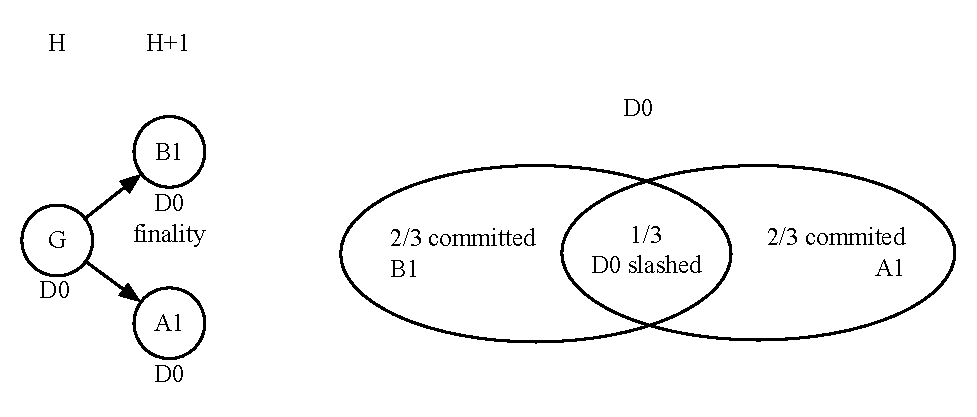
\includegraphics[width=11cm]{./figs/revert1}
\caption{Revert One Block by Short-range Attack}
\label{fig:revert1}
\end{figure}

Assume that B1 and B2 have reached the status of finality and transactions in the blocks have come into effect. If Attacker wants to revert B1-B2, the following two circumstances are taken into consideration. 

\begin{itemize}
\item The first circumstance is shown in Figure \ref{fig:revert2} (a): When Heights H+1 and H+2 are in the same Epoch and dynasty, Attacker needs to bribe $1/3$ of the validators in D0 in order to make A1 reach finality. Meanwhile, these $1/3$ of the validators will be punished and their deposits will be totally confiscated. During validation of A2, sum of deposits equals to $2/3$ of deposits in A1. At this moment, if Attacker wants to secure the same amount of commit votes as B2, he/she has to bribe all the remaining validators without cheating and lose at least $3/3$ of the total deposits. Even if Attacker succeeds in doing this, it is impossible to guarantee that score of A1 is higher than that of B1 and Attacker will face a high risk of failure of attack. 

\item The second circumstance is shown in Figure \ref{fig:revert2} (b): When Heights H+1 and H+2 are in different Epochs and different dynasties, Attacker needs to bribe $1/3$ of the validators in D0 to make A1 reach finality and then bribe $1/3$ of the validators in D1 to make A2 reach finality, so Attacker will lose at least $2/3$ of the total deposits in order to complete such an attack. To sum up, to launch a short-range attack to cause invalidation of two blocks that have reached finality, Attacker needs to pay at least $2/3$ of the total deposits. 
\end{itemize}
%如果Attacker想要使B1-B2失效,假设B1和B2都已到达finality,块中交易都已生效,为了让这些交易失效,这里考虑两种情况。第一种如图\ref{fig:revert2}中(a)所示,高度H+1和H+2在同一个Epoch中,朝代相同,那么Attacker首先需要贿赂D0中$1/3$的验证者使A1达到finality,此时这$1/3$的验证者将会被惩罚,押金被罚完。在A2的验证中整体押金总和只有A1中的$2/3$,此时Attacker想要让A2到达和B2同价值的committ票,需要贿赂剩下所有没有作弊的验证者,合起来至少需要损失总押金的$3/3$,即使如此也不能保证A1得分比B1高,攻击失败风险高。第二种情况如图\ref{fig:revert2}中(b)所示,高度H+1和H+2正好在不同的Epoch中,且朝代不相同,那么此时Attacker需要贿赂D0中的$1/3$来让A1到达finality,然后贿赂D1中的$1/3$来让A2达到finality,完成一次这样的攻击至少需要损失总押金的$2/3$。综上,想要发起短程攻击导致两个finality区块失效,至少需要花费总押金$2/3$的代价。

\begin{figure}[h]
\centering
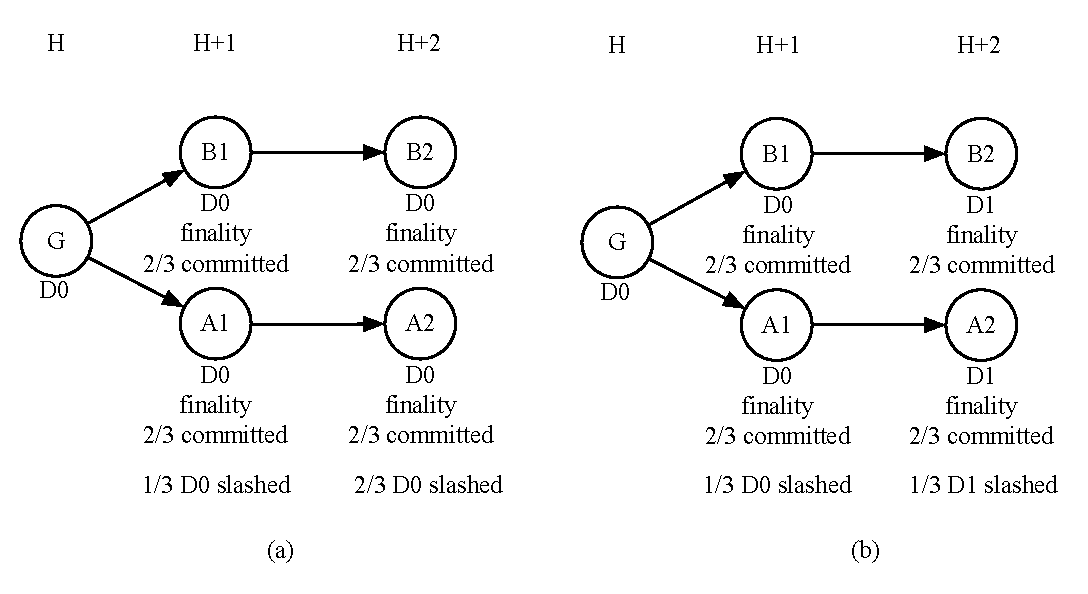
\includegraphics[width=11cm]{./figs/revert2}
\caption{Revert Two Blocks by Short-range Attack}
\label{fig:revert2}
\end{figure}

If Attacker wants to revert B1-B3, as shown in Figure 18, Attacker needs to firstly bribe $1/3$ of the validators in D0 in order to realize finality of A1 and then bribe $1/3$ of the validators in D1 in order to realize finality of A2. Finally, Attacker needs to bribe all of the remaining $2/3$ of the validators in D1 in order to realize finality of A3. To sum up, $4/3$ of the total amount of deposits will be lost. It will be very difficult to prepare for these attacks. Even if an attacker manages to succeed in making necessary preparations, he/she can’t guarantee that score of A1 is higher than that of B1. Therefore, it is possible that such attack may fail.

%如果Attacker想要使B1-B3失效,如图\ref{fig:revert3}所示,Attacker首先需要贿赂D0中$1/3$的人完成A1的finality,然后贿赂D1中$1/3$的人完成A2的finality,最后需要贿赂D1中剩下$2/3$中的所有人来完成A3的finality,综上至少要损失总押金的$4/3$。要完成这些攻击准备将会十分困难,而且即使有幸做到了,也不定能保证A1的得分比B1高,攻击也可能会失败。

\begin{figure}[h]
\centering
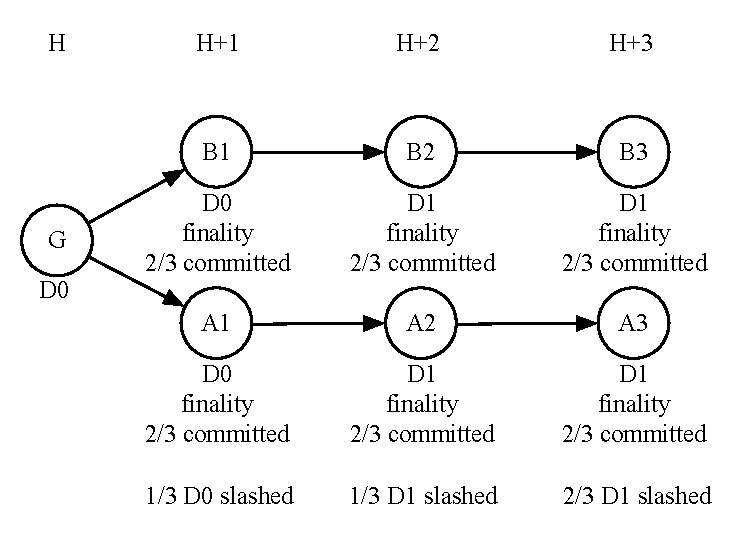
\includegraphics[width=7.5cm]{./figs/revert3}
\caption{Revert Three Blocks by Short-range Attack}
\label{fig:revert3}
\end{figure}

If Attacker wants to revert B1-BN, in which N is limited by term of expiration time of consensus of the block and thus can't be a very large number. When $N = 3$, the total deposits of all validators in the current dynasty will be totally confiscated. Therefore, when $N >= 4$, it is impossible to complete an attack in order to make score of B1 higher than that of A1 and revert B1-BN. It is pointless to launch such an attack.

%如果Attacker想要使B1-BN失效,其中N受到区块共识有效期的限制,不会很大,由于$N=3$时当前朝代所有验证者的押金就会被全部罚完,所以$N>=4$时,将没法完成攻击让B1得分比A1高,使B1-BN失效,发起这样的攻击没有任何意义。
 %TRADUCIDO
\newpage
\section{Motor de búsquedas en el blockchain}
\label{sec:search}

\subsection{Introducción}

As an increasing number of smart contracts are deployed by developers, searching needs for massive smart contracts soar. Given that smart contracts are simply code and include no functional descriptions, indexing smart contracts with search engine technologies imposes a high difficulty. To index smart contracts properly, we use the following methods:

\begin{itemize}
	\item Crawl webpage data relevant to smart contracts to set up mappings between the data and blockchain smart contracts.

	\item Encourage developers to upload verified source code of smart contracts, analyze the functions and semantics of the code, create indexes for the source code, and provide the searching function for similar contracts. For smart contracts without source code, decompile them for their source code.

	\item Establish standards for smart contracts so that any contracts matching those standards can be retrieved and found by users. Also, encourage developers to provide informational descriptions of contracts during smart contract creation. \\

	\begin{figure}[ht]
  	\centering
  	\begin{minipage}{.4\linewidth}
	\begin{lstlisting}[frame=single]
contract SearchableContract {
   string public language;
   string public author;
   string public name;
   string public title;
   string public description;
   string public tags;
}
	\end{lstlisting}
  	\end{minipage}
	\end{figure}

\end{itemize}

\subsection{Infrastructure}

In current stage, We think that the centralized search engine is more suitable for obtaining the best user experience and presenting the value of Nebulas Rank. The Nebulas development team is dedicated to developing a searching service, retrieving all smart contracts in real time, performing multilingual word breaking and creating full-text indexes to provide users with a user-friendly web interface. The impartiality of the NR ranking algorithm and the verifiability of each node ensure the impartiality of the centralized searching service, while the complete code of the searching backend is available to the community. Also, third-party developers can create their own searching services on this basis. \reffig{fig:search-arch} shows the architecture of the searching service.

\begin{figure}[h]
\centering
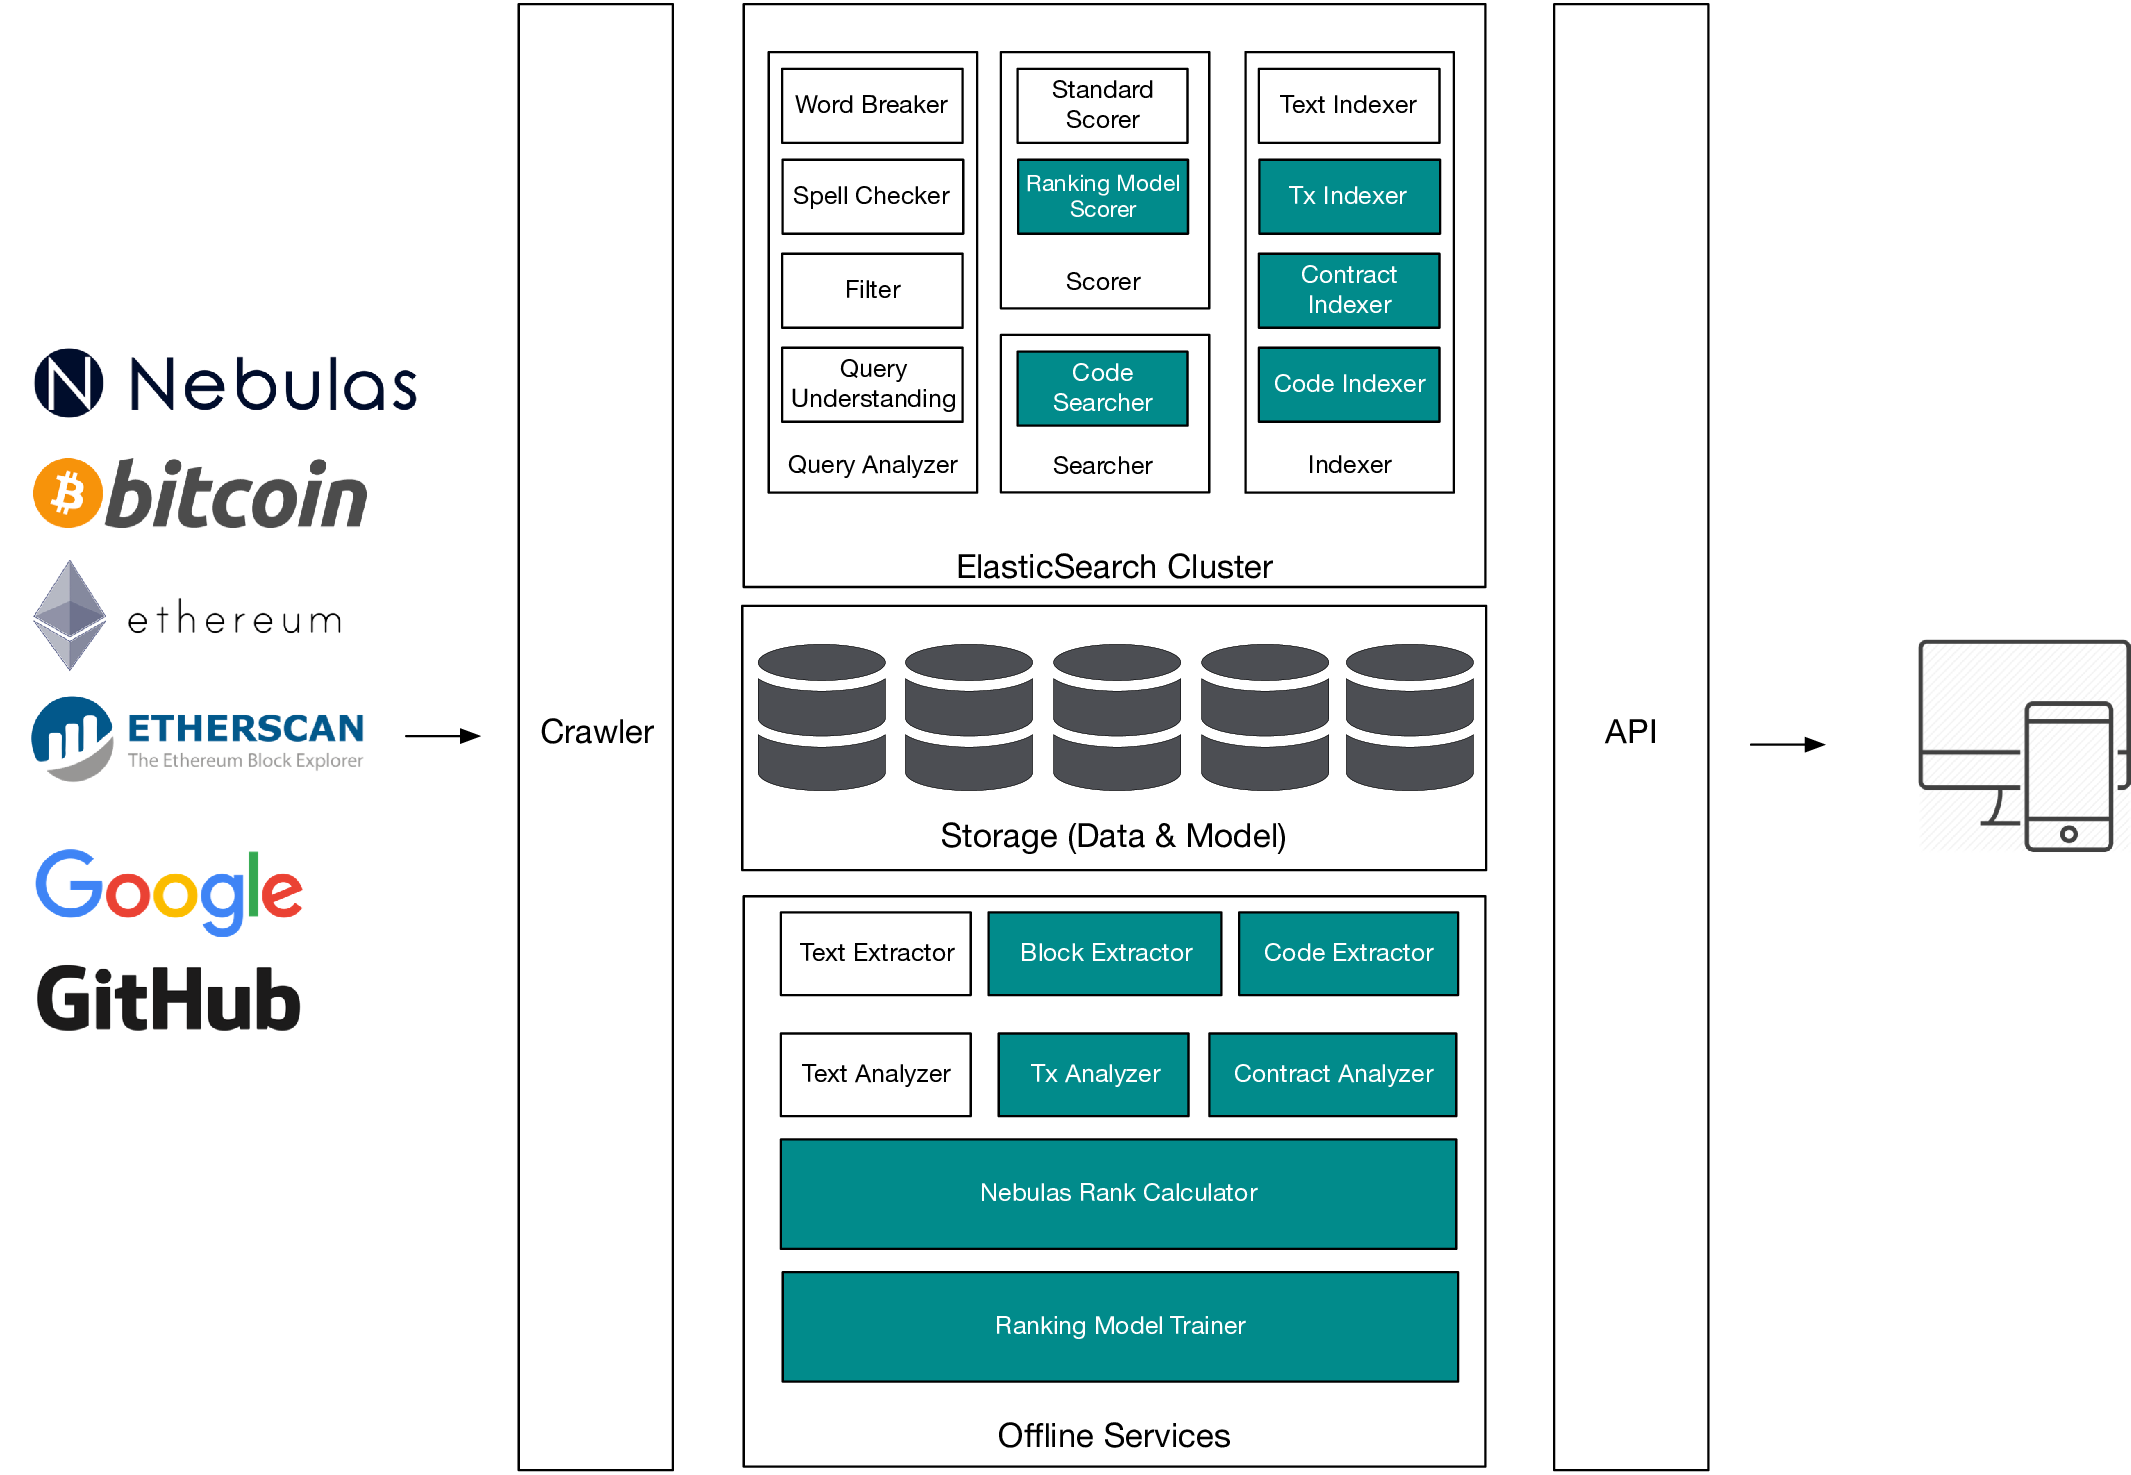
\includegraphics[width=16cm]{./figs/search-arch-new}
\caption{Architecture of the searching service}
\label{fig:search-arch}
\end{figure}

\begin{itemize}
	\item \textbf{Crawler}  data sources of the Crawler in blockchain search engine are classified into two types: one for collecting block information and code of smart contracts from blockchains, while the other for crawling data about smart contracts from public URLs including introductions, Dapp user comments and news.

	\item \textbf{Extractor} consists of Text Extractor, Block Extractor and Code Extractor, which provide text information, block information and code extraction service for smart contracts, respectively.

	\item \textbf{Analyzer} consists of Text Analyzer, Tx Analyzer and Contract Analyzer, which are text information, block transaction information and smart contract analyzers, respectively. For the smart contract analyzer, it provides contract decompilation, source code extraction, semantic analysis and so on.

	\item \textbf{Nebulas Rank Calculator} refers to the Nebulas Rank calculator service, which is used to calculate the Nebulas Ranks of each non-contract and contract accounts offline.

	\item \textbf{Ranking Model Trainer} refers to the ranking model trainer service. Ranking rules take multiple factors into account: matching field, text relevance, NR Rank value of the contract, transaction quantity of the contract, frequency and depth, NR Rank of the user conducting a transaction with the contract, and contract security. Based on users' actual use conditions, the machine learning algorithm (GBDT and artificial neural network (ANN) are optional) is used to train the ranking and scoring model, which is also constantly improved according to user feedback. The trained model is used by Scorer of the searching service.

	\item \textbf{Query Analyzer} refers to the keyword analysis service, which includes the multilingual word breaker (Word Breaker) and the spell checker (Spell Checker).

	\item \textbf{Indexer} creates proper indexes from Analyzer and supports both full and incremental indexing.

	\item \textbf{Scorer} is classified into two levels: Level-1 Standard Scorer recalls candidate result sets from ElasticSearch, which is done to recall as many candidate results as possible through the efficient and effective ranking in the ElasticSearch cluster. Level-1 can recall several thousands of results. Level-2 Ranking Model Scorer uses the offline rank model to calculate and reorder the rank of each Level-1 candidate result set. For this level, the calculated results feature a sounding accuracy and can be used directly by users.

	\item \textbf{Searcher} is responsible for communicating with the ElasticSearch cluster and packing and returning the search result to the searching frontend.

	\item \textbf{API} provides external applications with comprehensive searching API services.

	\item \textbf{ElasticSearch Cluster} ES refers to the server cluster. The Nebulas development team plans to use the open-source search engine ElasticSearch to support full-text indexing.

\end{itemize}

\subsection{Nebulas Trends}

The Nebulas creates the tendency list in combination with Nebulas Rank to provide user visual multi-dimensional values in blockchains.

\begin{itemize}
\item \textbf{Nebulas Rank list for non-contract accounts.} It displays the daily NR list and the NR quick rise and drop lists. Also, this rank list visualizes the rank variation tendency of each account and the health change tendency of the entire network.

\item \textbf{Nebulas Rank list for contract accounts.} Based on the NR values of non-contract accounts, the Nebulas Rank list calculates the NR list of contract accounts, the quick rise and drop lists, the variation tendency of each contract and the tendency chart for the quantity and use frequency of smart contracts on the entire network. In addition, we will present other smart contract lists such as the token contract list and the market contract estimation list to display a wider dimension of information.

\item \textbf{Smart contract developer list.} According to the contract account list, the list of smart contract developers calculates the contribution list of contract developers and the contribution quick rise list to display outstanding contracts developers and Dapps.

\end{itemize}

\subsection{Keyword Query}

By providing a keyword or describing the textual information about a smart contract such as its title, author or function, users can find the matching contract from massive smart contracts. Currently, mature and sophisticated algorithms and technologies are available for text searching. By using the natural language processing and inverted index technologies, we can retrieve and sort efficiently in the index database for massive smart contracts. This involves the following key technologies:

\begin{enumerate}
	\item Topic-oriented distributed crawler technology
	\item Multilingual word breaking technology: word breaking is relatively simple for western words. For the word breaking of Chinese words, these algorithms are available: positive maximum matching, negative maximum matching, shortest path word breaking and statistical word breaking.
	\item Search term correction and semantic comprehension
	\item Inverted index and distributed searching architecture
	\item Ranking algorithm to sort the search results

\end{enumerate}

Among these technologies, the ranking algorithm will be designed in combination with Nebulas Rank. Specifically, we use intra-user transfers in the blockchain world as an analogy to webpage reference relations in the Internet world to create the blockchain transaction graph. Then, calculate the NR rank of non-contract accounts by using the NR ranking algorithm described in Section 2.3, calculate the ranks of those contracts by using the contract ranking algorithm described in Section 4.2, and lastly use the calculation result for search result sorting.


\subsection{Searching for Similar Smart Contracts}

For developers and certain users, they may want to search for smart contracts with similar functions according to the code fragment of a contract. Being different from regular keyword searching, code similarity has its particularity. To implement the searching function for similar smart contracts, we need to use a certain algorithm to measure the code similarity in a number or percentage.

In today's academia, code similarity algorithms are mainly categorized into the string edit distance, token sequence similarity, abstract syntax tree similarity and program dependency graph similarity. These algorithms describe the similarity in terms of code text, structure and syntax from different dimensions. By combining these 4 major algorithms, we put forward 12 features of the code similarity of Nebulas contracts, such as Skeleton Tree, Type Signature and Library Calls. For details, see Appendix \ref{appendix:sim_code}.

Similar to search results of keywords, search results of smart contracts also use the same contract ranking algorithm to sort final results. %TRADUCIDO
\newpage
\section{基础服务及开发工具}
\label{sec:tools}

\subsection{域名服务}

在区块链的世界中,应用都以账号为中心,由于区块链的匿名性,账号地址是非常长的无意义的字符串,并不是用户友好的。用户可能容易出错,意外地投入资金导致丢失,或者与错误对象互动。如果用户能够使用容易记忆的域名,将是巨大的优势。星云链团队将会在链上用智能合约实现一个类似DNS的域名系统,称为NNS(Nebulas Name Service),保证其自由、免费、开放。任何第三方开发者可以独立地或者基于NNS实现自己的域名解析服务。

例如,alice为她的账号地址 0xdf4d22611412132d3e9bd322f82e2940674ec1bc03b20e40 申请了域名alice.nns,Bob如果想转账给alice,在收款人信息中只要填写alice.nns即可,钱包会通过NNS服务,把资金转账到正确的收款人地址。

NNS的申请规则如下:
\begin{itemize}
	\item 一级子域名保留,不可申请,例如*.nns,*.com,*.org,*.edu等等,用户只能申请二级子域名。
	\item NNS服务开放后,用户可以查询域名是否已经被占用。如果未被占用,可以通过智能合约提出竞价。竞价是公开的,任何人都可以查询其他人的竞价并且随时更新自己的竞价。
	\item 竞价期结束以后,价高者得此域名,智能合约会锁定用户的竞价资金。域名有效期为一年。一年后用户自由决定是否续约,同意续约后,有效期再延长一年。如果不续约,竞价资金自动退回用户账户,域名数据清空,重新变为可用。
	\item 用户可以随时放弃域名所有权,竞价资金自动退回用户账户,域名数据清空,重新变为可用。
	\item 用户可以无偿或者有偿转让域名所有权,域名之间的交易,星云链不做任何干预。
\end{itemize}


\subsection{闪电网络}
当前所有的公有链网络都面临系统的扩展性问题,例如比特币网络每秒只能处理7个交易,以太坊每秒处理15个交易。引入类PoS的共识算法,可以避免挖矿计算,大大加快共识速度,但是面对现实世界的海量微支付场景,公有链仍然面临极大的挑战。闪电网络~\cite{poon2015bitcoin}于2015年2月被提出,设计思路是为交易双方建立一个微支付通道网络,双方大量的支付都可以在链外直接多次、高频、双向地通过轧差方式实现瞬间确认。当交易结果需要结算时,再把最终结果提交到区块链确认,理论上可以实现每秒百万笔的转账。双方若无直接的点对点支付通道,只要网络中存在一条连通双方的、由多个支付通道构成的支付路径,也可以利用这条支付路径实现资金在双方之间的可靠转移。闪电网络在比特币和以太坊上都已经有概念性的验证。

星云链把闪电网络当做区块链的基础设施予以实现,并且提供足够的灵活性设计。任何第三方开发者,都可以在星云链上利用闪电网络的基础服务,做高频交易场景的应用开发。星云链也将发布世界首款支持闪电网络的钱包App。

\subsection{开发者工具}
完善的开发者工具,对于区块链应用开发者来说是非常重要的。目前各种公有区块链的开发者工具链都不够完善,对于大多数开发者是很大的阻碍。星云链开发组将提供丰富的开发者工具,包括独立的智能合约开发IDE,区块浏览器,各种流行IDE的插件支持(包括Eclipse, JetBrains, Visual Studio, Sublime Text, VIM, Atom等),调试器,模拟器,智能合约形式化验证工具,各种高级语言的后台SDK,移动端SDK等。
 %TRADUCIDO
\newpage
\section{星云链代币NAS}
\label{sec:nascoin}

星云链网络包含自身的内置货币星云币(NAS)。星云币在网络中体现两个作用:第一,星云币作为网络中的原生货币,提供用户之间的资产流动性,也作为记账人和DIP激励计划的奖励货币;第二,作为运行智能合约的运算费用收取。星云币的最小单位是$10^{-18}NAS$。

星云币最初在以太坊平台上以ERC20代币的方式发售,货币总量最大值为$X=10^8$枚,发行模式如下:
\begin{enumerate}
	\item \textbf{社区售卖:}
	
在星云链发起团队主导下,依照项目开发计划和需求,将分批次通过售卖的形式把大部分星云币分配给社区。首次面向社区影响力投资人售卖的星云币数量为$5\%X$,公开ICO售卖形式分配的星云币数量不少于$45\%X$。

	\item \textbf{创始\&开发团队激励:}

星云链的创始\&开发团队将在星云链的发展过程中,从项目组织架构,技术研发,生态运营上持续做出人力、物力资源的贡献。在代币分配机制上,预留出$20\%X$的部分作为团队激励。这部分星云币初始为锁定状态,自星云币首次面向社区售卖完成一年后开始解除锁定,分三年逐步分发至创始\&开发团队。

	\item \textbf{运营生态建设:}

除去以上两种分配方式,不超过$30\%X$的星云币将被用在星云链运营发展和生态建设中,包括但不局限于:DApp生态孵化、开发者社区建设、商业合作、市场推广、学术、教育、法律法规以及机构投资。
\end{enumerate}

星云链网络正式上线后,所有持有以太坊ERC20 NAS币的用户可以根据凭证,领取星云链网络的等量的星云币,同时以太坊的ERC20 NAS币被回收。随着星云链网络的演化,星云币增长如下:
\begin{enumerate}
	\item \textbf{记账人激励:}
	每年奖励给记账人的星云币数量为$3\%X$;
	
	\item \textbf{DIP激励:}
	每年奖励给优秀智能合约开发者的星云币数量为$2\%X$。
\end{enumerate} %TRADUCIDO
\newpage
\section{Conclusion}
\label{sec:conclusion}

\subsubsection*{What We Hold}

From a highly abstract perspective, blockchain is \textbf{the right confirmation of data in a decentralized way}, and tokens function as \textbf{the carrier of right confirmation value}. The Internet solves the communication of data, while blockchain further solves the right confirmation of data. For the first time ever, blockchain translates public data into private data which will no longer be analyzed and utilized arbitrarily by large enterprises such as Google, Amazon and Facebook.

%区块链从一种高度抽象的角度来看是一种\textbf{用去中心化的方式对于数据的确权},代币本身是对于\textbf{确权价值的载体}。互联网解决了数据的通讯问题,而区块链则在互联网上层进一步解决了数据的确权问题。区块链前所未有第一次让大家的数据真正变成自己的数据,而不再被BAT等大公司任意分析并使用。

The essence of blockchain represented by public blockchain is \textbf{``Community + Token + Application"}. Community is essentially a from-bottom-to-top ecosystem adhering to the idea of openness, open source, sharing and non-profitability, which is completely different from existing from-top-to-bottom business ecosystems. Token is the carrier of right confirmation value. There will be more scenarios in the future than those used only for attributes of virtual currency and electronic cash. Application simply refer to the technological implementation of blockchain application scenarios. Without the combination with the aforementioned two factors, application alone \textbf{cannot fully reflect the charm of blockchain systems}.

%以公有链为代表的区块链本质精神是:\textbf{社群+代币+工具}。社群本质上是自下而上,秉承的是开放、开源、共享、非盈利的理念,和现有自上而下的商业生态有着根本的不同。代币即是对于确权价值的载体,未来会有更多的应用场景,而远非是仅仅面向虚拟货币,电子现金的属性。工具仅仅是对于区块链应用场景具体技术实施,如缺少前两者的结合,其单独来看\textbf{并不能完全体现区块链系统的魅力所在}。

The blockchain system represented by public blockchain is the future of blockchain, as its \textbf{``trustless"} and \textbf{``permissionless"} attributes are the actual value of blockchain systems. On the contrary, most consortium blockchain/enterprise blockchain are \textbf{``trust-based"} and \textbf{``permission-based"}, which means they cannot break existing patterns and are considered as improved innovations. While public blockchain systems overturn existing cooperation relations and are considered \textbf{disruptive innovations}, reflecting the maximum value of blockchain.

%以公有链为代表的区块链体系才是区块链的未来,因为其本身所具有的“\textbf{非信任}”、“\textbf{无特权}”的基本特性才是区块链系统真正的价值所在。恰恰相反,作为联盟链/企业链大多具有“\textbf{基于信任}”和“\textbf{基于特权}”的属性,不能突破既有的范式,属于改良式创新。而公有链系统颠覆了既有的协作关系,属于\textbf{颠覆式创新},是区块链价值最大化的真正体现。

\subsubsection*{What We Are Committed To}

Be as the first blockchain search engine around the world, Nebulas is committed to \textbf{exploring hidden dimensions of blockchain value} and building value-based blockchain operating systems, search engines and other related extensive apps.

%作为全球首个区块链搜索引擎,星云链致力于\textbf{发掘区块链世界价值新维度},打造基于价值尺度的区块链操作系统、搜索引擎及其他相关扩展应用。

With this commitment, we put forward \textbf{Nebulas Rank} to set up the measure of value of the blockchain world, design \textbf{Nebulas Force} to empower the self-evolving of blockchains, develop \textbf{Developer Incentive Protocol} and \textbf{Proof of Devotion} to motivate the upgrade of blockchain value, and construct \textbf{Nebulas Search Engine} to help users explore other dimensions of blockchain value.

%基于此,我们提出Nebulas Rank星云指数来构建区块链世界的价值尺度,设计Nebulas Force星云原力来赋予区块链自我进化的能力,推出Developer Incentive Protocol开发者激励计划和Proof of Devotion贡献度共识证明来激励区块链的价值升级,打造Nebulas Search Engine区块链搜索引擎来帮助用户发现区块链上沉淀的多维度价值。

\subsubsection*{What We Believe}

The ongoing scientific and technological evolving will lead us to a better life with a higher level of \textbf{freedom and equality}. As one of the major technologies, blockchain will gradually give full play to its advantages. Being part of this evolving is our greatest happiness and accomplishment.

%正在发生科技浪潮会带领人们抵达更为\textbf{自由、平等、和美好}的生活。区块链作为其中重要的技术之一,会愈来愈散发出其特有的光彩和能量。能参与并投身其中,是我们最大的快乐和成就。

Similar to the Internet, blockchains will also enter a phase of explosive users/apps. Blockchain technology will become the \textbf{base protocol} of the next-generation ``smart network", and the number of users will reach or even go beyond one billion in the next 5 to 10 years. Significant opportunities and challenges will both emerge in the next five years.

%类似互联网对于世界的改变,区块链也即将面对其用户/应用临界值爆发的阶段。区块链技术会是下一代“智能网络”的\textbf{基础协议},整体用户规模会在5-10年内达到或超过10亿。未来的5年内会面临重大的机遇与挑战!

Facing the tremendous ecosystem in the future, ask not what blockchain can do for you, ask what you can do for blockchain. Because \textbf{blockchain is an organism and economy}. We are glad to share these with all of you in the exploration of blockchain technologies.

%在未来的巨大生态面前,在当下,不要问区块链能为你做什么,而是要问你能为区块链做什么。因为,\textbf{区块链本身就是生命体,区块链本身就是经济体}!在区块链技术探索的道路上,与诸君共勉!
 %TRADUCIDO
\bibliography{reference} %PENDIENTE

\begin{appendices}
\section{账号和地址}

\subsection{地址校验码设计}
类似于比特币和以太坊,星云链的帐号也是由椭圆曲线算法作为其基础加密算法。
用户的私钥是随机生成的256位二进制数,通过椭圆曲线乘法生成64字节的公钥。
比特币和以太坊的地址都是由公钥通过确定性的哈希算法运算得到,不同的是:比特币地址有校验码设计,防止用户输错了几个字符而把比特币误发给其它用户,以太坊却没有校验码设计。

我们认为从用户的角度看,校验码的设计是合理的,因此星云链的地址也包含了校验码,具体计算方法如下:

\begin{verbatim}
  Data = sha3_256(Public Key)[-20:]
  CheckSum = sha3_256(Data)[0:4]
  Address = "0x" + Data + CheckSum
\end{verbatim}

公钥的SHA3-256摘要的后20位字节作为地址的主要组成部分,对其再做一次SHA3-256摘要,取前四位字节做校验码,其相当于在以太坊的地址尾部加上四字节的校验码。

以太坊地址包括0x前缀共42位字符,星云链地址增加了8位字符的校验码,共50位字符。
	
\subsection{扩展地址验证}
除了支持50字符的标准地址,为了用户转账的安全,我们还支持扩展地址。借鉴了传统银行转账的设计:转账时除了验证对方的银行卡账号,汇款人还必须输入对方的姓名,只有银行卡账号和姓名都匹配,转账才能正确进行。扩展地址的生成算法如下:

\begin{verbatim}
  Address = "0x" + Data + CheckSum
  Ext = sha3_256(Data + nick)[0:2]
  ExtAddress = Address + Ext
\end{verbatim}

扩展地址在标准地址的尾部追加了2字节的扩展验证,共54位字符。加入扩展信息,使得在星云链钱包应用中可以增加另一个要素验证。例如:
\begin{enumerate}
	\item Alice的钱包标准地址是0x5d65d971895edc438f465c17db6992698a52318d5c17db69,加入昵称“alice”后的扩展地址是0x5d65d971895edc438f465c17db6992698a52318d5c17db69aabb;
	\item Alice告诉Bob扩展地址 0x5d65d971895edc438f465c17db6992698a52318d5c17db69aabb和昵称"alice";
	\item Bob在Wallet应用中,输入 0x5d65d971895edc438f465c17db6992698a52318d5c17db69aabb和alice;
	\item Wallet应用验证钱包地址的一致性,避免Bob错误的输成了其它人的帐号。
\end{enumerate}
		
标准地址和扩展地址均可以用于转账,我们的星云链钱包应用将会强制使用扩展地址,转账时需要提供对方的昵称,验证地址一致性,进一步加强安全校验。
 %TRADUCIDO
\section{Búsqueda de contratos inteligentes similares}
\label{appendix:sim_code}

La dificultad en la búsqueda de similaridad de código radica en las características estructurales de los lenguajes de alto nivel, y en la diversidad de las expresiones lógicas de los contratos inteligentes. En la actualidad existen varias escuelas de algoritmos de búsqueda de similaridad de código en los círculos académicos, las que se describen de este modo:

\begin{itemize}
	\item \textbf{Distancia de edición entre cadenas de caracteres} \\
	Tanto la consulta de código como el código fuente candidato se consideran como texto. La distancia de edición entre dos cadenas de caracteres se utiliza para medir las similitudes entre ambos. La \textit{distancia de edición} se refiere al número mínimo ded operaciones de edición necesarias para convertir una cadena de caracteres en otra. Las operaciones de edición permitidas incluyen la sustitución de un carácter por otro —borrado de un carácter e inserción de otro—. Generalmente hablando, a menor distancia de edición, mayor la similitud entre dos cadenas de caracteres. Este algoritmo basado en distancias de edición entre cadenas de caracteres puede ser usado no sólo para la comparación de códigos fuente sino también en representaciones intermedias o incluso código de máquina.
	Con el fin de mejorar la robustez de estos algoritmos, se llevará a cabo un cierto grado de conversión del código fuente sin introducir cambios semánticos: esto puede ser la remoción de caracteres en blanco, la remoción de comentarios, el reemplazo de los nombres de todas las variables locales con ‘\$’, la normalización de las expresiones algebraicas, etcétera. Este tipo de algoritmos se caracterizan por ser veloces, concisos y muy eficientes. No obstante, su adaptabilidad a programas complejos es relativamente pobre y no tienen en cuenta la sintaxis y la estructura organizativa del código.

	\item \textbf{Secuencia de tokens} \\
	El método de representación de secuencias de tokens se refiere a la conversión del código fuente ingresado en una secuencia de tokens a través del análisis léxico. La similitud entre dos programas se puede ver como la similitud entre dos secuencias de tokens, de modo que se puede utilizar la mayor subcadena en común o un algoritmo de coincidencia de correlación (algoritmo de coincidencia de árboles de sufijos) para medir el grado de similitud entre dos programas, a través del cual se pueden detectar segmentos de código con diferentes sintaxis pero con funciones similares. Sin embargo, este método oculta la estructura organizativa de los programas al medir la similitud entre ellos.

	\item \textbf{Árbol de sintaxis abstracta (\textit{Abstract Syntax Tree}, o AST)} \\
	AST es una forma de expresión intermedia después de realizar un análisis sintáctico en un código fuente, sobre el cual se puede medir la similitud entre dos programas a través de la comparación entre un subárbol y otro. Para medir la similitud entre dos árboles se puede utilizar el algoritmo de distancia de edición de árbol \cite{zhang1989simple}. El algoritmo preciso de la distancia de edición del árbol es relativamente complejo y la literatura al respecto (\cite{guha2002approximate}) proporciona un algoritmo rápido aproximado. De acuerdo a \cite{chilowicz2009syntax}, los árboles de sintaxis deben someterse a una identificación por huella hash con el fin de habilitar al algoritmo de comparación del árbol de sintaxis para realizar búsquedas de alta eficiencia en conjuntos de datos masivos.

	\item \textbf{Grafo de dependencias de programas (\textit{Program Dependency Graph}, o PDG)} \\
	Un PDG \cite{ferrante1987program} puede representar los datos internos, controlar la relación de dependencia de un programa y analizar el código de programa a nivel semántico. Un protocolo de código similar se transforma en una búsqueda de subgrafos isomórficos, que es un problema NP-completo y requiere un algoritmo muy complejo, por lo que sólo algunos algoritmos aproximados están disponibles en la actualidad.

\end{itemize}

Creemos que los algoritmos mencionados describen las similitudes entre códigos en texto, estructura y sintaxis en dimensiones diferentes. Source Forager \cite{kashyap2017source} nos proporciona un gran ejercicio mental: los índices de similitud en distintas dimensiones se representan como características diferentes, cada una de las cuales representa la medición de la similitud del código desde un aspecto específico. Por último, la similitud vectorial se utiliza para llevar a cabo la medición de la similitud general. Este método integra las ventajas de los algoritmos mencionados anteriormente. Esta idea también es utilizada por Nebulas como referencia para realizar la búsqueda de la similitud entre contratos inteligentes. Consideramos que funciona como la unidad fundamental de búsqueda de código entre los contratos inteligentes.

La tabla \ref{table:search-similarity} define las características de similitud entre códigos candidatos. Luego, se describe la definición de cada característica y la función para calcular su similitud:

\begin{table}[h]
\centering
\begin{threeparttable}[b]
\caption{Tabla de familias de características de similitud de código}
\label{table:search-similarity}
\begin{tabular}{ccc} \toprule
    {Clase de características} & {Descripción} \\ \midrule
Emparejamiento tipo-operación & Tipos empleados y operaciones realizadas sobre esos tipos \\
Esqueleto de árbol & Estructura de bucles y condicionales \\
Esqueleto de árbol decorado & Estructura de bucles, condicionales y operaciones \\
BFS sobre 3-grafo del CFG & Subgrafos de un CFG de tamaño 3, usando BFS para generar subgrafos \\
BFS sobre 4-grafo del CFG & Subgrafos de un CFG de tamaño 4, usando BFS para generar subgrafos \\
DFS sobre 3-grafo del CFG & Subgrafos de un CFG de tamaño 3, usando DFS para generar subgrafos \\
DFS sobre 4-grafo del CFG & Subgrafos de un CFG de tamaño 4, usando DFS para generar subgrafos \\
Llamadas a librerías & Llamadas a librerías \\
Signatura & Tipos de entrada y valor devuelto \\
Tipos locales & Tipos de las variables locales \\
Literales numéricos & Constantes de datos numéricos \\
Literal de cadena & Constantes de datos de cadena \\
\bottomrule
\end{tabular}
\end{threeparttable}
\end{table}

\begin{itemize}
	\item \textbf{\textit{Emparejamiento tipo-operación}} \\
	Es un conjunto 2-tupla que contiene el tipo de la variable y su operador, es decir, el par (tipo, operación). Generalmente, los tipos de datos primitivos debe emparejarse con un operador aritmético, un operador lógico y un operador relacional, tal como ($int, \geq$); los tipos de datos personalizados (como las estructuras \texttt{struct}) deben emparejarse con las funciones miembro, tales como (\texttt{Bar}, \texttt{.foo}), indicando que el campo \texttt{foo} del tipo de dato \texttt{Bar} es consultado. Basándonos en esta metodología, todas las operaciones sobre variables en el cuerpo del código de una función se deben transformar en 2-tuplas.

	Después de eliminar repeticiones, se utiliza una secuencia 2-tupla para reflejar la característica de emparejamiento tipo-operación de este segmento de código. Creemos que las piezas de código con funciones similares deben tener similares conjuntos de operaciones sobre variables. No obstante, no nos preocupa el orden de las 2-tuplas, por lo que esta característica pierde la información de la estructura lógica del código y por lo tanto sólo puede representar parcialmente sus características.

	La similitud entre las características de emparejamiento tipo-operación se puede definir mediante similitudes Jacobianas; es decir que dados dos conjuntos $S_1$ y $S_2$, la similitud Jacobiana se puede definir mediante la siguiente fórmula:

	\begin{equation}
	sim_{Jacc(S_{1}, S_{2})}=\frac{\mid S_{1}\bigcap S_{2}\mid}{\mid S_{1}\bigcup S_{2}\mid}
	\end{equation}

	\item Esqueleto de árbol (\textit{Skeleton Tree}) \\
	Árbol de sintaxis abstracta basado en código. Sólo se mantienen las estructuras de bucle (\texttt{for, while, do...while}) y las sentencias condicionales (\texttt{if...else}); todos los otros nodos son removidos del árbol. Creemos que los códigos con funciones similares deberían ser similares en cuanto a estructuras de bucle y sentencias condicionales.

	El cálculo de la similitud para esqueletos de árbol está basado en la distancia de edición entre dos árboles. Se define $d_{r}$ como la distancia de edición estimada entre dos árboles, y está determinada únicamente por el tamaño del árbol, es decir:

	\begin{equation}
	d_{r}(T_{1}, T{2})=\frac{\mid size(T_{1})-size(T_{2})\mid}{max(size(T_{1}), size(T_{2}))}
	\end{equation}

	Se asume $D_T$ como el valor umbral de la distancia de edición, y se fija en 0,5. Podemos adquirir la fórmula para el cálculo de la distancia aproximada de edición entre dos árboles:

	\begin{equation}
	d_{t}(T_{1}, T{2})=\begin{cases}d_{r}(T_{1}, T{2}) & if~d_{r}(T_{1}, T{2})\geq D_{T}\\\frac{max\left(\begin{array}{c}ed(pre(T_{1}),~pre(T_{2})),\\ ed(post(T_{1}),~post(T_{2}))\end{array}\right)}{max(size(T_{1}), size(T_{2}))} & otherwise\end{cases}
	\end{equation}

	$pre(T)$ representa la secuencia transversal del árbol antes de la ordenación; $post(T)$ representa la secuencia transversal del árbol después de la ordenación; $ed(S_{1}, S_{2})$ representa la distancia de edición entre $S_{1}$ y $S_{2}$. La similitud entre dos esqueletos de árbol se puede calcular mediante la siguiente fórmula:

	\begin{equation}
	sim_{Tree}(T_{1}, T{2})=1-d_{t}(T_{1}, T{2})
	\end{equation}

	\item Esqueleto de árbol decorado (\textit{Decorated Skeleton Tree}) \\
	Esta entidad es similar al esqueleto de árbol, aunque además de preservar los nodos de bucle y bifurcación, se conservan la mayoría de los operadores (tales como \texttt{+, -, <}), excepto por \texttt{=} y \texttt{\&}, considerados como \textit{ruido}.

	\item \textbf{K-subgrafos del CFG} \\
	Dado un CFG\footnote{CFG aquí refiere a la locución inglesa \textit{Control Flow Graph}, es decir, grafo de flujo de control (N. del T.)} y un nodo específico, se lleva a cabo una búsqueda BFS\footnote{\textit{Breadth-First Search}, o \textit{búsqueda en anchura} (N. del T.)} o bien una búsqueda DFS\footnote{\textit{Depth-First Search}, o \textit{búsqueda en profundidad} (N. del T.)} hasta que el número de nodos recorridos llegue a $k$, momento en el cual el subgrafo formado debería ser el k-subgrafo. Si el número de nodos no llega a $k$ luego de finalizar el recorrido, dicho subgrafo se debe descartar. Mediante el recorrido de cada nodo en el CFG, podemos adquirir todos los k-subgrafos. Por cada k-subgrafo, es necesario utilizar un entero de $k^2$ bits para expresarlo. Para más detalles, consúltese la \ref{fig:graph-ex}. Todos los k-subgrafos forman un conjunto de enteros.

	\textbf{BFS sobre 3-grafo del CFG:} k = 3, recorrido de árbol BFS

	\textbf{BFS sobre 4-grafo del CFG:} k = 4, recorrido de árbol BFS

	\textbf{DFS sobre 3-grafo del CFG:} k = 3, recorrido de árbol DFS

	\textbf{DFS sobre 4-grafo del CFG:} k = 4, recorrido de árbol DFS

	Dados los vectores $\vec{x}=(x_{1}, x_{2}, ...x_{n})$ y $\vec{y}=(y_{1}, y_{2}, ...y_{n})$, la similitud Jacobiana generalizada se puede definir como:

	\begin{equation}
	J(\vec{x}, \vec{y})=\frac{\sum_imin(x_{i}, y_{i})}{\sum_imax(x_{i}, y_{i})}
	\end{equation}

	\begin{figure}[h]
	\centering
	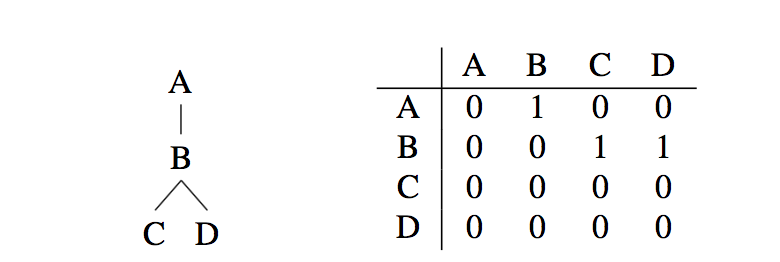
\includegraphics[width=6cm]{./figs/graph-matrix.png}
	\caption{Ejemplo para un 4-grafo: el elemento de la matriz es la cadena binaria \texttt{0100 0011 0000 0000}, que representa el número decimal es 17 152}
	\label{fig:graph-ex}
	\end{figure}

	\item \textbf{Llamadas a librerías} \\
	Si dentro del contrato se realiza una llamada a un contrato-librería, se registrarán las direcciones de todos los contratos-librería, y la similitud se calculará mediante la fórmula de similitud Jacobiana.

	\item \textbf{Signatura} \\
	Consiste en registrar el tipo de los parámetros y el tipo del valor de retorno de la función; la similitud se calcula mediante la fórmula de similitud Jacobiana. Por ejemplo, para el siguiente código de un contrato inteligente, la característica \textit{signatura} de la función \texttt{getBalance} es el vector \texttt{(address, uint256)}. \\

	\begin{figure}[h]
  	\centering
  	\begin{minipage}{.7\linewidth}
	\begin{lstlisting}[frame=single]
contract addressTest {
  function getBalance(address addr) returns (uint) {
  	return addr.balance;
  }
}
	\end{lstlisting}
  	\end{minipage}
	\end{figure}

	\item \textbf{Tipos locales:} esta característica es el conjunto de todos los tipos de las variables locales de la función \texttt{body}, para el que debe calcularse la similitud mediante la fórmula de similitud Jacobiana.

	\item \textbf{Literales numéricos:} el conjunto de todas las constantes numéricas sirve como la característica de los \textit{literales numéricos}, para el que debe calcularse la similitud mediante la fórmula de similitud Jacobiana.

	\item \textbf{Literales de cadena:} el conjunto de todas las constantes de cadena sirve como la característica de los \textit{literales de cadena}, para el que debe calcularse la similitud mediante la fórmula de similitud Jacobiana.
\end{itemize}

La familia de características se puede expandir, por lo que es conveniente añadir nuevas características a ella. Basándonos en la circunstancia de que existe un cálculo de similitud por cada característica, podemos calcular la suma ponderada de todas las características y así adquirir la similitud final del código:

\begin{equation}
	sim_{combined}(\vec{A}, \vec{B})=\frac{\sum_{c=1}^{n_{cl}}sim_{c}(\vec{A_c},~\vec{B_c})\cdot w_{c}}{\sum_{c=1}^{n_{cl}}w_{c}}
\end{equation}

En donde $\vec{A}$ y $\vec{B}$ son vectores propios; $n_{cl}$ es el número de características en la familia; $sim_{c}$ es la función de cálculo de similitud específica de la característica c; $\vec{A_c}$ y $\vec{B_c}$ son vectores propios de la característica c; $w_{c}$ es la ponderación de c. La ponderación se puede hallar mediante el entrenamiento de algoritmos de aprendizaje de máquinas basado en un gran número de equipos de prueba. %EN PROCESO
\end{appendices}

\end{document}